\section{Limits of Functions}

\begin{definition}
We say $f$ as a function of $x$ has a limit $L$ at $c \in \mathbb{R}$, denoted by
\begin{align*}
    &\lim_{x \longrightarrow c} f(x) = L \hspace{4pt} \text{if} \hspace{20pt} &&\text{for all} \hspace{4pt} \epsilon > 0, \hspace{4pt} \text{there exists a} \hspace{4pt} \delta > 0 \hspace{4pt} \text{such that}\\[2ex]
    &\text{for all} \hspace{4pt} x \in \text{Dom($f$)} \hspace{4pt} \text{satisfying} \hspace{4pt} \lvert x - c \rvert < \delta &&\text{we have} \hspace{4pt} \lvert f(x) - L \rvert < \epsilon
\end{align*}
\end{definition}

% This file was created with tikzplotlib v0.10.1.


\documentclass{article}
\usepackage[utf8]{inputenc}

% Standard math packages
\usepackage{amsmath}
\usepackage{amsthm}
\usepackage{amssymb}
\usepackage{amsfonts} 

% Package for the layout
\usepackage{geometry}

% Packages for the tikzplotlib library
\usepackage{tikz}
\usepackage{pgfplots}
\usepackage{pgfplotstable}
\pgfplotsset{compat=1.7}
\usepackage{subcaption}
\usepgfplotslibrary{groupplots}


\begin{document}


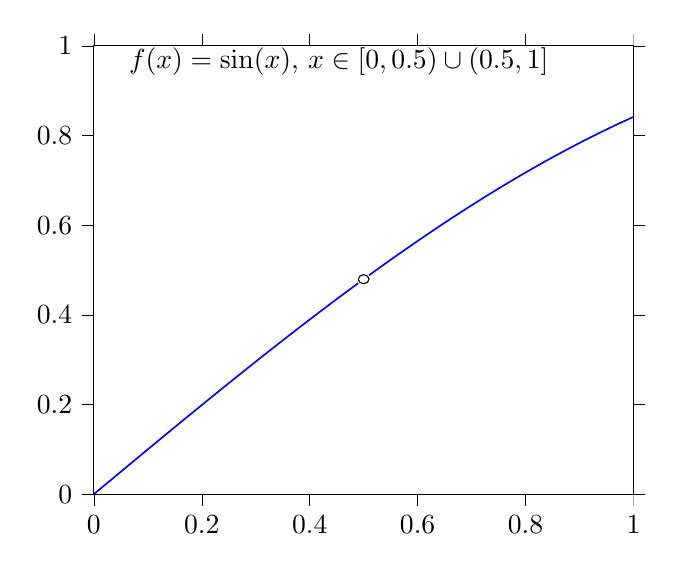
\begin{tikzpicture}

\definecolor{darkgray176}{RGB}{176,176,176}

\begin{axis}[
tick align=outside,
tick pos=both,
x grid style={darkgray176},
xmin=0, xmax=1,
xtick style={color=black},
y grid style={darkgray176},
ymin=0, ymax=1,
ytick style={color=black}
]
\draw[draw=black] (axis cs:0.5,0.479425538604203) circle (0.01);
\addplot [semithick, blue]
table {%
0 0
9.80196039207842e-05 9.80196037638247e-05
0.000196039207841568 0.000196039206585892
0.000294058811762352 0.000294058807524446
0.000392078415683137 0.000392078405637729
0.000490098019603921 0.000490097999983985
0.000588117623524705 0.000588117589621456
0.000686137227445489 0.000686137173608385
0.000784156831366273 0.000784156751003017
0.000882176435287057 0.000882176320863594
0.000980196039207842 0.000980195882248359
0.00107821564312863 0.00107821543421556
0.00117623524704941 0.00117623497582343
0.00127425485097019 0.00127425450613022
0.00137227445489098 0.00137227402419418
0.00147029405881176 0.00147029352907354
0.00156831366273255 0.00156831301982655
0.00166633326665333 0.00166633249551146
0.00176435287057411 0.00176435195518651
0.0018623724744949 0.00186237139790994
0.00196039207841568 0.00196039082274
0.00205841168233647 0.00205841022873494
0.00215643128625725 0.00215642961495299
0.00225445089017804 0.0022544489804524
0.00235247049409882 0.00235246832429143
0.0024504900980196 0.00245048764552831
0.00254850970194039 0.00254850694322128
0.00264652930586117 0.00264652621642861
0.00274454890978196 0.00274454546420853
0.00284256851370274 0.00284256468561928
0.00294058811762352 0.00294058387971912
0.00303860772154431 0.0030386030455663
0.00313662732546509 0.00313662218221905
0.00323464692938588 0.00323464128873563
0.00333266653330666 0.00333266036417428
0.00343068613722745 0.00343067940759326
0.00352870574114823 0.00352869841805081
0.00362672534506901 0.00362671739460519
0.0037247449489898 0.00372473633631463
0.00382276455291058 0.00382275524223739
0.00392078415683137 0.00392077411143172
0.00401880376075215 0.00401879294295586
0.00411682336467293 0.00411681173586808
0.00421484296859372 0.00421483048922662
0.0043128625725145 0.00431284920208973
0.00441088217643529 0.00441086787351566
0.00450890178035607 0.00450888650256266
0.00460692138427686 0.004606905088289
0.00470494098819764 0.00470492362975291
0.00480296059211842 0.00480294212601266
0.00490098019603921 0.0049009605761265
0.00499899979995999 0.00499897897915267
0.00509701940388078 0.00509699733414945
0.00519503900780156 0.00519501564017507
0.00529305861172234 0.0052930338962878
0.00539107821564313 0.0053910521015459
0.00548909781956391 0.00548907025500761
0.0055871174234847 0.0055870883557312
0.00568513702740548 0.00568510640277492
0.00578315663132627 0.00578312439519704
0.00588117623524705 0.0058811423320558
0.00597919583916783 0.00597916021240947
0.00607721544308862 0.00607717803531632
0.0061752350470094 0.00617519579983459
0.00627325465093019 0.00627321350502255
0.00637127425485097 0.00637123114993846
0.00646929385877175 0.00646924873364059
0.00656731346269254 0.00656726625518719
0.00666533306661332 0.00666528371363653
0.00676335267053411 0.00676330110804687
0.00686137227445489 0.00686131843747648
0.00695939187837568 0.00695933570098362
0.00705741148229646 0.00705735289762656
0.00715543108621724 0.00715537002646356
0.00725345069013803 0.00725338708655289
0.00735147029405881 0.00735140407695282
0.0074494898979796 0.00744942099672161
0.00754750950190038 0.00754743784491754
0.00764552910582116 0.00764545462059887
0.00774354870974195 0.00774347132282388
0.00784156831366273 0.00784148795065083
0.00793958791758352 0.007939504503138
0.0080376075215043 0.00803752097934366
0.00813562712542508 0.00813553737832608
0.00823364672934587 0.00823355369914353
0.00833166633326665 0.0083315699408543
0.00842968593718744 0.00842958610251665
0.00852770554110822 0.00852760218318887
0.00862572514502901 0.00862561818192923
0.00872374474894979 0.008723634097796
0.00882176435287057 0.00882164992984746
0.00891978395679136 0.00891966567714191
0.00901780356071214 0.0090176813387376
0.00911582316463293 0.00911569691369284
0.00921384276855371 0.00921371240106589
0.00931186237247449 0.00931172779991504
0.00940988197639528 0.00940974310929857
0.00950790158031606 0.00950775832827477
0.00960592118423685 0.00960577345590193
0.00970394078815763 0.00970378849123832
0.00980196039207842 0.00980180343334224
0.0098999799959992 0.00989981828127198
0.00999799959991998 0.00999783303408581
0.0100960192038408 0.010095847690842
0.0101940388077616 0.010193862250599
0.0102920584116823 0.0102918767124148
0.0103900780156031 0.010389891075348
0.0104880976195239 0.0104879053384567
0.0105861172234447 0.0105859195007993
0.0106841368273655 0.010683933561434
0.0107821564312863 0.0107819475194192
0.010880176035207 0.0108799613738131
0.0109781956391278 0.010977975123674
0.0110762152430486 0.0110759887680603
0.0111742348469694 0.0111740023060303
0.0112722544508902 0.0112720157366421
0.011370274054811 0.0113700290589543
0.0114682936587317 0.0114680422720249
0.0115663132626525 0.0115660553749125
0.0116643328665733 0.0116640683666751
0.0117623524704941 0.0117620812463713
0.0118603720744149 0.0118600940130592
0.0119583916783357 0.0119581066657972
0.0120564112822565 0.0120561192036436
0.0121544308861772 0.0121541316256567
0.012252450490098 0.0122521439308948
0.0123504700940188 0.0123501561184163
0.0124484896979396 0.0124481681872793
0.0125465093018604 0.0125461801365424
0.0126445289057812 0.0126441919652637
0.0127425485097019 0.0127422036725016
0.0128405681136227 0.0128402152573144
0.0129385877175435 0.0129382267187605
0.0130366073214643 0.0130362380558981
0.0131346269253851 0.0131342492677855
0.0132326465293059 0.0132322603534812
0.0133306661332266 0.0133302713120434
0.0134286857371474 0.0134282821425305
0.0135267053410682 0.0135262928440007
0.013624724944989 0.0136243034155124
0.0137227445489098 0.013722313856124
0.0138207641528306 0.0138203241648937
0.0139187837567514 0.0139183343408799
0.0140168033606721 0.014016344383141
0.0141148229645929 0.0141143542907352
0.0142128425685137 0.014212364062721
0.0143108621724345 0.0143103736981565
0.0144088817763553 0.0144083831961003
0.0145069013802761 0.0145063925556106
0.0146049209841968 0.0146044017757457
0.0147029405881176 0.014702410855564
0.0148009601920384 0.0148004197941239
0.0148989797959592 0.0148984285904837
0.01499699939988 0.0149964372437017
0.0150950190038008 0.0150944457528363
0.0151930386077215 0.0151924541169459
0.0152910582116423 0.0152904623350887
0.0153890778155631 0.0153884704063232
0.0154870974194839 0.0154864783297077
0.0155851170234047 0.0155844861043005
0.0156831366273255 0.0156824937291601
0.0157811562312462 0.0157805012033447
0.015879175835167 0.0158785085259127
0.0159771954390878 0.0159765156959225
0.0160752150430086 0.0160745227124325
0.0161732346469294 0.016172529574501
0.0162712542508502 0.0162705362811863
0.016369273854771 0.0163685428315469
0.0164672934586917 0.0164665492246412
0.0165653130626125 0.0165645554595274
0.0166633326665333 0.0166625615352639
0.0167613522704541 0.0167605674509092
0.0168593718743749 0.0168585732055216
0.0169573914782957 0.0169565787981595
0.0170554110822164 0.0170545842278812
0.0171534306861372 0.0171525894937452
0.017251450290058 0.0172505945948098
0.0173494698939788 0.0173485995301334
0.0174474894978996 0.0174466042987743
0.0175455091018204 0.0175446088997911
0.0176435287057411 0.017642613332242
0.0177415483096619 0.0177406175951854
0.0178395679135827 0.0178386216876798
0.0179375875175035 0.0179366256087835
0.0180356071214243 0.0180346293575549
0.0181336267253451 0.0181326329330525
0.0182316463292659 0.0182306363343345
0.0183296659331866 0.0183286395604595
0.0184276855371074 0.0184266426104858
0.0185257051410282 0.0185246454834718
0.018623724744949 0.0186226481784759
0.0187217443488698 0.0187206506945566
0.0188197639527906 0.0188186530307721
0.0189177835567113 0.018916655186181
0.0190158031606321 0.0190146571598417
0.0191138227645529 0.0191126589508125
0.0192118423684737 0.019210660558152
0.0193098619723945 0.0193086619809184
0.0194078815763153 0.0194066632181702
0.019505901180236 0.0195046642689658
0.0196039207841568 0.0196026651323637
0.0197019403880776 0.0197006658074223
0.0197999599919984 0.0197986662932
0.0198979795959192 0.0198966665887552
0.01999599919984 0.0199946666931464
0.0200940188037608 0.0200926666054319
0.0201920384076815 0.0201906663246703
0.0202900580116023 0.0202886658499199
0.0203880776155231 0.0203866651802392
0.0204860972194439 0.0204846643146867
0.0205841168233647 0.0205826632523207
0.0206821364272855 0.0206806619921997
0.0207801560312062 0.0207786605333821
0.020878175635127 0.0208766588749265
0.0209761952390478 0.0209746570158912
0.0210742148429686 0.0210726549553347
0.0211722344468894 0.0211706526923154
0.0212702540508102 0.0212686502258919
0.0213682736547309 0.0213666475551225
0.0214662932586517 0.0214646446790657
0.0215643128625725 0.02156264159678
0.0216623324664933 0.0216606383073238
0.0217603520704141 0.0217586348097556
0.0218583716743349 0.0218566311031338
0.0219563912782557 0.021954627186517
0.0220544108821764 0.0220526230589636
0.0221524304860972 0.022150618719532
0.022250450090018 0.0222486141672808
0.0223484696939388 0.0223466094012684
0.0224464892978596 0.0224446044205533
0.0225445089017804 0.022542599224194
0.0226425285057011 0.0226405938112489
0.0227405481096219 0.0227385881807765
0.0228385677135427 0.0228365823318354
0.0229365873174635 0.022934576263484
0.0230346069213843 0.0230325699747807
0.0231326265253051 0.0231305634647842
0.0232306461292258 0.0232285567325528
0.0233286657331466 0.0233265497771451
0.0234266853370674 0.0234245425976197
0.0235247049409882 0.0235225351930348
0.023622724544909 0.0236205275624492
0.0237207441488298 0.0237185197049212
0.0238187637527506 0.0238165116195095
0.0239167833566713 0.0239145033052724
0.0240148029605921 0.0240124947612686
0.0241128225645129 0.0241104859865565
0.0242108421684337 0.0242084769801946
0.0243088617723545 0.0243064677412415
0.0244068813762753 0.0244044582687556
0.024504900980196 0.0245024485617956
0.0246029205841168 0.0246004386194199
0.0247009401880376 0.024698428440687
0.0247989597919584 0.0247964180246555
0.0248969793958792 0.024894407370384
0.0249949989998 0.0249923964769309
0.0250930186037207 0.0250903853433548
0.0251910382076415 0.0251883739687142
0.0252890578115623 0.0252863623520676
0.0253870774154831 0.0253843504924737
0.0254850970194039 0.0254823383889909
0.0255831166233247 0.0255803260406779
0.0256811362272455 0.025678313446593
0.0257791558311662 0.025776300605795
0.025877175435087 0.0258742875173423
0.0259751950390078 0.0259722741802936
0.0260732146429286 0.0260702605937073
0.0261712342468494 0.0261682467566421
0.0262692538507702 0.0262662326681564
0.0263672734546909 0.026364218327309
0.0264652930586117 0.0264622037331582
0.0265633126625325 0.0265601888847628
0.0266613322664533 0.0266581737811812
0.0267593518703741 0.0267561584214722
0.0268573714742949 0.0268541428046941
0.0269553910782156 0.0269521269299057
0.0270534106821364 0.0270501107961654
0.0271514302860572 0.027148094402532
0.027249449889978 0.0272460777480639
0.0273474694938988 0.0273440608318198
0.0274454890978196 0.0274420436528583
0.0275435087017403 0.0275400262102379
0.0276415283056611 0.0276380085030173
0.0277395479095819 0.0277359905302551
0.0278375675135027 0.0278339722910098
0.0279355871174235 0.0279319537843401
0.0280336067213443 0.0280299350093045
0.0281316263252651 0.0281279159649618
0.0282296459291858 0.0282258966503705
0.0283276655331066 0.0283238770645892
0.0284256851370274 0.0284218572066765
0.0285237047409482 0.0285198370756911
0.028621724344869 0.0286178166706916
0.0287197439487898 0.0287157959907366
0.0288177635527105 0.0288137750348847
0.0289157831566313 0.0289117538021947
0.0290138027605521 0.029009732291725
0.0291118223644729 0.0291077105025344
0.0292098419683937 0.0292056884336815
0.0293078615723145 0.0293036660842249
0.0294058811762352 0.0294016434532234
0.029503900780156 0.0294996205397354
0.0296019203840768 0.0295975973428198
0.0296999399879976 0.029695573861535
0.0297979595919184 0.0297935500949399
0.0298959791958392 0.029891526042093
0.02999399879976 0.0299895017020531
0.0300920184036807 0.0300874770738787
0.0301900380076015 0.0301854521566286
0.0302880576115223 0.0302834269493614
0.0303860772154431 0.0303814014511358
0.0304840968193639 0.0304793756610105
0.0305821164232847 0.0305773495780441
0.0306801360272054 0.0306753232012954
0.0307781556311262 0.030773296529823
0.030876175235047 0.0308712695626855
0.0309741948389678 0.0309692422989418
0.0310722144428886 0.0310672147376505
0.0311702340468094 0.0311651868778702
0.0312682536507301 0.0312631587186598
0.0313662732546509 0.0313611302590778
0.0314642928585717 0.031459101498183
0.0315623124624925 0.0315570724350342
0.0316603320664133 0.0316550430686899
0.0317583516703341 0.031753013398209
0.0318563712742548 0.0318509834226501
0.0319543908781756 0.0319489531410719
0.0320524104820964 0.0320469225525333
0.0321504300860172 0.0321448916560928
0.032248449689938 0.0322428604508093
0.0323464692938588 0.0323408289357414
0.0324444888977796 0.032438797109948
0.0325425085017003 0.0325367649724877
0.0326405281056211 0.0326347325224192
0.0327385477095419 0.0327326997588014
0.0328365673134627 0.032830666680693
0.0329345869173835 0.0329286332871527
0.0330326065213043 0.0330265995772392
0.033130626125225 0.0331245655500114
0.0332286457291458 0.0332225312045279
0.0333266653330666 0.0333204965398477
0.0334246849369874 0.0334184615550293
0.0335227045409082 0.0335164262491315
0.033620724144829 0.0336143906212133
0.0337187437487498 0.0337123546703332
0.0338167633526705 0.0338103183955502
0.0339147829565913 0.0339082817959229
0.0340128025605121 0.0340062448705102
0.0341108221644329 0.0341042076183708
0.0342088417683537 0.0342021700385636
0.0343068613722745 0.0343001321301473
0.0344048809761952 0.0343980938921807
0.034502900580116 0.0344960553237227
0.0346009201840368 0.0345940164238319
0.0346989397879576 0.0346919771915674
0.0347969593918784 0.0347899376259877
0.0348949789957992 0.0348878977261518
0.0349929985997199 0.0349858574911184
0.0350910182036407 0.0350838169199465
0.0351890378075615 0.0351817760116947
0.0352870574114823 0.035279734765422
0.0353850770154031 0.0353776931801871
0.0354830966193239 0.035475651255049
0.0355811162232446 0.0355736089890663
0.0356791358271654 0.035671566381298
0.0357771554310862 0.0357695234308029
0.035875175035007 0.0358674801366398
0.0359731946389278 0.0359654364978677
0.0360712142428486 0.0360633925135452
0.0361692338467694 0.0361613481827314
0.0362672534506901 0.036259303504485
0.0363652730546109 0.036357258477865
0.0364632926585317 0.0364552131019301
0.0365613122624525 0.0365531673757392
0.0366593318663733 0.0366511212983513
0.0367573514702941 0.0367490748688252
0.0368553710742148 0.0368470280862197
0.0369533906781356 0.0369449809495938
0.0370514102820564 0.0370429334580063
0.0371494298859772 0.0371408856105161
0.037247449489898 0.0372388374061822
0.0373454690938188 0.0373367888440633
0.0374434886977396 0.0374347399232185
0.0375415083016603 0.0375326906427066
0.0376395279055811 0.0376306410015864
0.0377375475095019 0.037728590998917
0.0378355671134227 0.0378265406337573
0.0379335867173435 0.037924489905166
0.0380316063212643 0.0380224388122023
0.038129625925185 0.0381203873539249
0.0382276455291058 0.0382183355293928
0.0383256651330266 0.038316283337665
0.0384236847369474 0.0384142307778003
0.0385217043408682 0.0385121778488578
0.038619723944789 0.0386101245498963
0.0387177435487097 0.0387080708799748
0.0388157631526305 0.0388060168381523
0.0389137827565513 0.0389039624234876
0.0390118023604721 0.0390019076350398
0.0391098219643929 0.0390998524718678
0.0392078415683137 0.0391977969330306
0.0393058611722344 0.0392957410175871
0.0394038807761552 0.0393936847245963
0.039501900380076 0.0394916280531171
0.0395999199839968 0.0395895710022086
0.0396979395879176 0.0396875135709298
0.0397959591918384 0.0397854557583395
0.0398939787957592 0.0398833975634969
0.0399919983996799 0.0399813389854608
0.0400900180036007 0.0400792800232903
0.0401880376075215 0.0401772206760444
0.0402860572114423 0.0402751609427821
0.0403840768153631 0.0403731008225624
0.0404820964192839 0.0404710403144442
0.0405801160232046 0.0405689794174867
0.0406781356271254 0.0406669181307488
0.0407761552310462 0.0407648564532896
0.040874174834967 0.040862794384168
0.0409721944388878 0.0409607319224431
0.0410702140428086 0.0410586690671739
0.0411682336467293 0.0411566058174195
0.0412662532506501 0.0412545421722389
0.0413642728545709 0.0413524781306912
0.0414622924584917 0.0414504136918353
0.0415603120624125 0.0415483488547304
0.0416583316663333 0.0416462836184355
0.0417563512702541 0.0417442179820097
0.0418543708741748 0.0418421519445119
0.0419523904780956 0.0419400855050014
0.0420504100820164 0.0420380186625371
0.0421484296859372 0.0421359514161781
0.042246449289858 0.0422338837649835
0.0423444688937788 0.0423318157080124
0.0424424884976995 0.0424297472443239
0.0425405081016203 0.0425276783729771
0.0426385277055411 0.042625609093031
0.0427365473094619 0.0427235394035447
0.0428345669133827 0.0428214693035775
0.0429325865173035 0.0429193987921882
0.0430306061212242 0.0430173278684361
0.043128625725145 0.0431152565313804
0.0432266453290658 0.04321318478008
0.0433246649329866 0.0433111126135941
0.0434226845369074 0.0434090400309818
0.0435207041408282 0.0435069670313024
0.0436187237447489 0.0436048936136148
0.0437167433486697 0.0437028197769783
0.0438147629525905 0.0438007455204519
0.0439127825565113 0.0438986708430949
0.0440108021604321 0.0439965957439664
0.0441088217643529 0.0440945202221254
0.0442068413682737 0.0441924442766313
0.0443048609721944 0.0442903679065431
0.0444028805761152 0.04438829111092
0.044500900180036 0.0444862138888212
0.0445989197839568 0.0445841362393059
0.0446969393878776 0.0446820581614331
0.0447949589917984 0.0447799796542622
0.0448929785957191 0.0448779007168523
0.0449909981996399 0.0449758213482626
0.0450890178035607 0.0450737415475523
0.0451870374074815 0.0451716613137805
0.0452850570114023 0.0452695806460065
0.0453830766153231 0.0453674995432895
0.0454810962192439 0.0454654180046887
0.0455791158231646 0.0455633360292633
0.0456771354270854 0.0456612536160726
0.0457751550310062 0.0457591707641757
0.045873174634927 0.0458570874726319
0.0459711942388478 0.0459550037405004
0.0460692138427686 0.0460529195668404
0.0461672334466893 0.0461508349507113
0.0462652530506101 0.0462487498911722
0.0463632726545309 0.0463466643872823
0.0464612922584517 0.046444578438101
0.0465593118623725 0.0465424920426875
0.0466573314662933 0.0466404052001011
0.046755351070214 0.0467383179094009
0.0468533706741348 0.0468362301696464
0.0469513902780556 0.0469341419798967
0.0470494098819764 0.0470320533392112
0.0471474294858972 0.0471299642466491
0.047245449089818 0.0472278747012697
0.0473434686937387 0.0473257847021323
0.0474414882976595 0.0474236942482963
0.0475395079015803 0.0475216033388208
0.0476375275055011 0.0476195119727652
0.0477355471094219 0.0477174201491889
0.0478335667133427 0.0478153278671511
0.0479315863172635 0.0479132351257111
0.0480296059211842 0.0480111419239283
0.048127625525105 0.048109048260862
0.0482256451290258 0.0482069541355716
0.0483236647329466 0.0483048595471163
0.0484216843368674 0.0484027644945555
0.0485197039407882 0.0485006689769485
0.0486177235447089 0.0485985729933548
0.0487157431486297 0.0486964765428336
0.0488137627525505 0.0487943796244443
0.0489117823564713 0.0488922822372463
0.0490098019603921 0.0489901843802989
0.0491078215643129 0.0490880860526616
0.0492058411682336 0.0491859872533936
0.0493038607721544 0.0492838879815544
0.0494018803760752 0.0493817882362034
0.049499899979996 0.0494796880163999
0.0495979195839168 0.0495775873212033
0.0496959391878376 0.0496754861496731
0.0497939587917584 0.0497733845008686
0.0498919783956791 0.0498712823738493
0.0499899979995999 0.0499691797676745
0.0500880176035207 0.0500670766814037
0.0501860372074415 0.0501649731140963
0.0502840568113623 0.0502628690648117
0.0503820764152831 0.0503607645326094
0.0504800960192038 0.0504586595165488
0.0505781156231246 0.0505565540156893
0.0506761352270454 0.0506544480290904
0.0507741548309662 0.0507523415558116
0.050872174434887 0.0508502345949122
0.0509701940388078 0.0509481271454517
0.0510682136427285 0.0510460192064897
0.0511662332466493 0.0511439107770855
0.0512642528505701 0.0512418018562987
0.0513622724544909 0.0513396924431887
0.0514602920584117 0.051437582536815
0.0515583116623325 0.0515354721362372
0.0516563312662533 0.0516333612405146
0.051754350870174 0.0517312498487068
0.0518523704740948 0.0518291379598732
0.0519503900780156 0.0519270255730735
0.0520484096819364 0.0520249126873671
0.0521464292858572 0.0521227993018134
0.052244448889778 0.0522206854154722
0.0523424684936987 0.0523185710274028
0.0524404880976195 0.0524164561366648
0.0525385077015403 0.0525143407423177
0.0526365273054611 0.0526122248434211
0.0527345469093819 0.0527101084390345
0.0528325665133027 0.0528079915282175
0.0529305861172234 0.0529058741100296
0.0530286057211442 0.0530037561835304
0.053126625325065 0.0531016377477794
0.0532246449289858 0.0531995188018363
0.0533226645329066 0.0532973993447605
0.0534206841368274 0.0533952793756117
0.0535187037407482 0.0534931588934495
0.0536167233446689 0.0535910378973334
0.0537147429485897 0.053688916386323
0.0538127625525105 0.053786794359478
0.0539107821564313 0.0538846718158579
0.0540088017603521 0.0539825487545223
0.0541068213642729 0.0540804251745309
0.0542048409681936 0.0541783010749433
0.0543028605721144 0.0542761764548191
0.0544008801760352 0.054374051313218
0.054498899779956 0.0544719256491994
0.0545969193838768 0.0545697994618232
0.0546949389877976 0.054667672750149
0.0547929585917183 0.0547655455132363
0.0548909781956391 0.0548634177501449
0.0549889977995599 0.0549612894599344
0.0550870174034807 0.0550591606416645
0.0551850370074015 0.0551570312943948
0.0552830566113223 0.0552549014171851
0.0553810762152431 0.0553527710090949
0.0554790958191638 0.055450640069184
0.0555771154230846 0.0555485085965121
0.0556751350270054 0.0556463765901388
0.0557731546309262 0.055744244049124
0.055871174234847 0.0558421109725271
0.0559691938387678 0.0559399773594081
0.0560672134426885 0.0560378432088266
0.0561652330466093 0.0561357085198422
0.0562632526505301 0.0562335732915148
0.0563612722544509 0.0563314375229041
0.0564592918583717 0.0564293012130698
0.0565573114622925 0.0565271643610716
0.0566553310662132 0.0566250269659694
0.056753350670134 0.0567228890268228
0.0568513702740548 0.0568207505426915
0.0569493898779756 0.0569186115126355
0.0570474094818964 0.0570164719357143
0.0571454290858172 0.0571143318109879
0.0572434486897379 0.057212191137516
0.0573414682936587 0.0573100499143583
0.0574394878975795 0.0574079081405747
0.0575375075015003 0.0575057658152249
0.0576355271054211 0.0576036229373688
0.0577335467093419 0.0577014795060661
0.0578315663132627 0.0577993355203767
0.0579295859171834 0.0578971909793603
0.0580276055211042 0.0579950458820768
0.058125625125025 0.0580929002275861
0.0582236447289458 0.0581907540149479
0.0583216643328666 0.0582886072432221
0.0584196839367874 0.0583864599114685
0.0585177035407081 0.058484312018747
0.0586157231446289 0.0585821635641175
0.0587137427485497 0.0586800145466397
0.0588117623524705 0.0587778649653735
0.0589097819563913 0.0588757148193789
0.0590078015603121 0.0589735641077157
0.0591058211642329 0.0590714128294437
0.0592038407681536 0.0591692609836229
0.0593018603720744 0.0592671085693131
0.0593998799759952 0.0593649555855743
0.059497899579916 0.0594628020314663
0.0595959191838368 0.0595606479060491
0.0596939387877576 0.0596584932083825
0.0597919583916783 0.0597563379375265
0.0598899779955991 0.0598541820925411
0.0599879975995199 0.059952025672486
0.0600860172034407 0.0600498686764213
0.0601840368073615 0.0601477111034069
0.0602820564112823 0.0602455529525028
0.060380076015203 0.0603433942227688
0.0604780956191238 0.0604412349132651
0.0605761152230446 0.0605390750230514
0.0606741348269654 0.0606369145511878
0.0607721544308862 0.0607347534967343
0.060870174034807 0.0608325918587508
0.0609681936387277 0.0609304296362974
0.0610662132426485 0.061028266828434
0.0611642328465693 0.0611261034342205
0.0612622524504901 0.0612239394527171
0.0613602720544109 0.0613217748829837
0.0614582916583317 0.0614196097240804
0.0615563112622525 0.061517443975067
0.0616543308661732 0.0616152776350038
0.061752350470094 0.0617131107029506
0.0618503700740148 0.0618109431779676
0.0619483896779356 0.0619087750591148
0.0620464092818564 0.0620066063454522
0.0621444288857772 0.0621044370360399
0.0622424484896979 0.0622022671299379
0.0623404680936187 0.0623000966262063
0.0624384876975395 0.0623979255239052
0.0625365073014603 0.0624957538220946
0.0626345269053811 0.0625935815198346
0.0627325465093019 0.0626914086161854
0.0628305661132226 0.0627892351102069
0.0629285857171434 0.0628870610009594
0.0630266053210642 0.0629848862875029
0.063124624924985 0.0630827109688974
0.0632226445289058 0.0631805350442033
0.0633206641328266 0.0632783585124804
0.0634186837367473 0.0633761813727891
0.0635167033406681 0.0634740036241894
0.0636147229445889 0.0635718252657414
0.0637127425485097 0.0636696462965053
0.0638107621524305 0.0637674667155413
0.0639087817563513 0.0638652865219095
0.0640068013602721 0.06396310571467
0.0641048209641928 0.0640609242928831
0.0642028405681136 0.0641587422556089
0.0643008601720344 0.0642565596019077
0.0643988797759552 0.0643543763308394
0.064496899379876 0.0644521924414645
0.0645949189837968 0.064550007932843
0.0646929385877175 0.0646478228040352
0.0647909581916383 0.0647456370541013
0.0648889777955591 0.0648434506821015
0.0649869973994799 0.064941263687096
0.0650850170034007 0.065039076068145
0.0651830366073215 0.0651368878243089
0.0652810562112422 0.0652346989546477
0.065379075815163 0.0653325094582219
0.0654770954190838 0.0654303193340915
0.0655751150230046 0.065528128581317
0.0656731346269254 0.0656259371989585
0.0657711542308462 0.0657237451860763
0.065869173834767 0.0658215525417307
0.0659671934386877 0.0659193592649819
0.0660652130426085 0.0660171653548904
0.0661632326465293 0.0661149708105162
0.0662612522504501 0.0662127756309199
0.0663592718543709 0.0663105798151616
0.0664572914582917 0.0664083833623017
0.0665553110622124 0.0665061862714005
0.0666533306661332 0.0666039885415183
0.066751350270054 0.0667017901717154
0.0668493698739748 0.0667995911610523
0.0669473894778956 0.0668973915085891
0.0670454090818164 0.0669951912133864
0.0671434286857372 0.0670929902745044
0.0672414482896579 0.0671907886910035
0.0673394678935787 0.0672885864619441
0.0674374874974995 0.0673863835863865
0.0675355071014203 0.0674841800633911
0.0676335267053411 0.0675819758920184
0.0677315463092619 0.0676797710713286
0.0678295659131826 0.0677775656003822
0.0679275855171034 0.0678753594782397
0.0680256051210242 0.0679731527039614
0.068123624724945 0.0680709452766077
0.0682216443288658 0.0681687371952391
0.0683196639327866 0.0682665284589159
0.0684176835367073 0.0683643190666987
0.0685157031406281 0.0684621090176479
0.0686137227445489 0.0685598983108239
0.0687117423484697 0.0686576869452871
0.0688097619523905 0.0687554749200982
0.0689077815563113 0.0688532622343174
0.0690058011602321 0.0689510488870053
0.0691038207641528 0.0690488348772224
0.0692018403680736 0.0691466202040291
0.0692998599719944 0.069244404866486
0.0693978795759152 0.0693421888636535
0.069495899179836 0.0694399721945922
0.0695939187837568 0.0695377548583625
0.0696919383876775 0.069635536854025
0.0697899579915983 0.0697333181806402
0.0698879775955191 0.0698310988372687
0.0699859971994399 0.069928878822971
0.0700840168033607 0.0700266581368076
0.0701820364072815 0.0701244367778391
0.0702800560112022 0.070222214745126
0.070378075615123 0.0703199920377289
0.0704760952190438 0.0704177686547084
0.0705741148229646 0.070515544595125
0.0706721344268854 0.0706133198580394
0.0707701540308062 0.0707110944425121
0.0708681736347269 0.0708088683476037
0.0709661932386477 0.0709066415723749
0.0710642128425685 0.0710044141158862
0.0711622324464893 0.0711021859771983
0.0712602520504101 0.0711999571553717
0.0713582716543309 0.0712977276494671
0.0714562912582516 0.0713954974585452
0.0715543108621724 0.0714932665816666
0.0716523304660932 0.0715910350178919
0.071750350070014 0.0716888027662818
0.0718483696739348 0.071786569825897
0.0719463892778556 0.071884336195798
0.0720444088817764 0.0719821018750457
0.0721424284856971 0.0720798668627007
0.0722404480896179 0.0721776311578236
0.0723384676935387 0.0722753947594753
0.0724364872974595 0.0723731576667163
0.0725345069013803 0.0724709198786073
0.0726325265053011 0.0725686813942092
0.0727305461092218 0.0726664422125826
0.0728285657131426 0.0727642023327882
0.0729265853170634 0.0728619617538869
0.0730246049209842 0.0729597204749392
0.073122624524905 0.073057478495006
0.0732206441288258 0.0731552358131481
0.0733186637327466 0.0732529924284262
0.0734166833366673 0.073350748339901
0.0735147029405881 0.0734485035466334
0.0736127225445089 0.0735462580476841
0.0737107421484297 0.073644011842114
0.0738087617523505 0.0737417649289837
0.0739067813562713 0.0738395173073541
0.074004800960192 0.0739372689762861
0.0741028205641128 0.0740350199348405
0.0742008401680336 0.074132770182078
0.0742988597719544 0.0742305197170595
0.0743968793758752 0.0743282685388458
0.074494898979796 0.0744260166464979
0.0745929185837167 0.0745237640390765
0.0746909381876375 0.0746215107156424
0.0747889577915583 0.0747192566752566
0.0748869773954791 0.07481700191698
0.0749849969993999 0.0749147464398734
0.0750830166033207 0.0750124902429976
0.0751810362072415 0.0751102333254137
0.0752790558111622 0.0752079756861824
0.075377075415083 0.0753057173243648
0.0754750950190038 0.0754034582390216
0.0755731146229246 0.0755011984292139
0.0756711342268454 0.0755989378940025
0.0757691538307662 0.0756966766324485
0.0758671734346869 0.0757944146436126
0.0759651930386077 0.075892151926556
0.0760632126425285 0.0759898884803395
0.0761612322464493 0.0760876243040241
0.0762592518503701 0.0761853593966707
0.0763572714542909 0.0762830937573405
0.0764552910582117 0.0763808273850942
0.0765533106621324 0.076478560278993
0.0766513302660532 0.0765762924380977
0.076749349869974 0.0766740238614695
0.0768473694738948 0.0767717545481694
0.0769453890778156 0.0768694844972583
0.0770434086817364 0.0769672137077973
0.0771414282856571 0.0770649421788473
0.0772394478895779 0.0771626699094696
0.0773374674934987 0.077260396898725
0.0774354870974195 0.0773581231456747
0.0775335067013403 0.0774558486493798
0.0776315263052611 0.0775535734089012
0.0777295459091818 0.0776512974233
0.0778275655131026 0.0777490206916374
0.0779255851170234 0.0778467432129745
0.0780236047209442 0.0779444649863723
0.078121624324865 0.0780421860108919
0.0782196439287858 0.0781399062855945
0.0783176635327065 0.0782376258095411
0.0784156831366273 0.078335344581793
0.0785137027405481 0.0784330626014111
0.0786117223444689 0.0785307798674567
0.0787097419483897 0.078628496378991
0.0788077615523105 0.078726212135075
0.0789057811562312 0.07882392713477
0.079003800760152 0.078921641377137
0.0791018203640728 0.0790193548612374
0.0791998399679936 0.0791170675861322
0.0792978595719144 0.0792147795508826
0.0793958791758352 0.0793124907545499
0.0794938987797559 0.0794102011961953
0.0795919183836767 0.07950791087488
0.0796899379875975 0.0796056197896651
0.0797879575915183 0.079703327939612
0.0798859771954391 0.0798010353237818
0.0799839967993599 0.0798987419412358
0.0800820164032807 0.0799964477910353
0.0801800360072014 0.0800941528722415
0.0802780556111222 0.0801918571839156
0.080376075215043 0.0802895607251191
0.0804740948189638 0.080387263494913
0.0805721144228846 0.0804849654923587
0.0806701340268054 0.0805826667165176
0.0807681536307261 0.0806803671664509
0.0808661732346469 0.0807780668412199
0.0809641928385677 0.0808757657398859
0.0810622124424885 0.0809734638615103
0.0811602320464093 0.0810711612051544
0.0812582516503301 0.0811688577698794
0.0813562712542509 0.0812665535547469
0.0814542908581716 0.0813642485588182
0.0815523104620924 0.0814619427811545
0.0816503300660132 0.0815596362208173
0.081748349669934 0.0816573288768679
0.0818463692738548 0.0817550207483677
0.0819443888777756 0.0818527118343782
0.0820424084816963 0.0819504021339607
0.0821404280856171 0.0820480916461766
0.0822384476895379 0.0821457803700873
0.0823364672934587 0.0822434683047543
0.0824344868973795 0.082341155449239
0.0825325065013003 0.0824388418026028
0.082630526105221 0.0825365273639072
0.0827285457091418 0.0826342121322136
0.0828265653130626 0.0827318961065835
0.0829245849169834 0.0828295792860784
0.0830226045209042 0.0829272616697597
0.083120624124825 0.0830249432566889
0.0832186437287458 0.0831226240459274
0.0833166633326665 0.0832203040365369
0.0834146829365873 0.0833179832275788
0.0835127025405081 0.0834156616181146
0.0836107221444289 0.0835133392072059
0.0837087417483497 0.0836110159939141
0.0838067613522705 0.0837086919773009
0.0839047809561912 0.0838063671564276
0.084002800560112 0.083904041530356
0.0841008201640328 0.0840017150981476
0.0841988397679536 0.0840993878588639
0.0842968593718744 0.0841970598115664
0.0843948789757952 0.0842947309553169
0.084492898579716 0.0843924012891769
0.0845909181836367 0.0844900708122079
0.0846889377875575 0.0845877395234716
0.0847869573914783 0.0846854074220297
0.0848849769953991 0.0847830745069436
0.0849829965993199 0.0848807407772751
0.0850810162032407 0.0849784062320858
0.0851790358071614 0.0850760708704373
0.0852770554110822 0.0851737346913913
0.085375075015003 0.0852713976940095
0.0854730946189238 0.0853690598773535
0.0855711142228446 0.085466721240485
0.0856691338267654 0.0855643817824656
0.0857671534306861 0.0856620415023572
0.0858651730346069 0.0857597003992213
0.0859631926385277 0.0858573584721197
0.0860612122424485 0.0859550157201141
0.0861592318463693 0.0860526721422663
0.0862572514502901 0.0861503277376378
0.0863552710542108 0.0862479825052906
0.0864532906581316 0.0863456364442863
0.0865513102620524 0.0864432895536868
0.0866493298659732 0.0865409418325537
0.086747349469894 0.0866385932799488
0.0868453690738148 0.086736243894934
0.0869433886777355 0.086833893676571
0.0870414082816563 0.0869315426239216
0.0871394278855771 0.0870291907360475
0.0872374474894979 0.0871268380120107
0.0873354670934187 0.087224484450873
0.0874334866973395 0.0873221300516961
0.0875315063012603 0.0874197748135419
0.087629525905181 0.0875174187354723
0.0877275455091018 0.0876150618165491
0.0878255651130226 0.0877127040558341
0.0879235847169434 0.0878103454523893
0.0880216043208642 0.0879079860052765
0.088119623924785 0.0880056257135576
0.0882176435287057 0.0881032645762944
0.0883156631326265 0.088200902592549
0.0884136827365473 0.0882985397613832
0.0885117023404681 0.0883961760818588
0.0886097219443889 0.0884938115530379
0.0887077415483097 0.0885914461739824
0.0888057611522304 0.0886890799437542
0.0889037807561512 0.0887867128614153
0.089001800360072 0.0888843449260276
0.0890998199639928 0.0889819761366531
0.0891978395679136 0.0890796064923537
0.0892958591718344 0.0891772359921915
0.0893938787757552 0.0892748646352285
0.0894918983796759 0.0893724924205265
0.0895899179835967 0.0894701193471478
0.0896879375875175 0.0895677454141542
0.0897859571914383 0.0896653706206077
0.0898839767953591 0.0897629949655705
0.0899819963992799 0.0898606184481046
0.0900800160032006 0.089958241067272
0.0901780356071214 0.0900558628221347
0.0902760552110422 0.0901534837117548
0.090374074814963 0.0902511037351945
0.0904720944188838 0.0903487228915158
0.0905701140228046 0.0904463411797807
0.0906681336267254 0.0905439585990514
0.0907661532306461 0.09064157514839
0.0908641728345669 0.0907391908268586
0.0909621924384877 0.0908368056335193
0.0910602120424085 0.0909344195674343
0.0911582316463293 0.0910320326276657
0.0912562512502501 0.0911296448132756
0.0913542708541708 0.0912272561233262
0.0914522904580916 0.0913248665568797
0.0915503100620124 0.0914224761129982
0.0916483296659332 0.091520084790744
0.091746349269854 0.0916176925891792
0.0918443688737748 0.091715299507366
0.0919423884776955 0.0918129055443666
0.0920404080816163 0.0919105106992432
0.0921384276855371 0.0920081149710582
0.0922364472894579 0.0921057183588736
0.0923344668933787 0.0922033208617518
0.0924324864972995 0.0923009224787549
0.0925305061012203 0.0923985232089454
0.092628525705141 0.0924961230513853
0.0927265453090618 0.092593722005137
0.0928245649129826 0.0926913200692628
0.0929225845169034 0.092788917242825
0.0930206041208242 0.0928865135248858
0.093118623724745 0.0929841089145077
0.0932166433286657 0.0930817034107528
0.0933146629325865 0.0931792970126836
0.0934126825365073 0.0932768897193623
0.0935107021404281 0.0933744815298514
0.0936087217443489 0.0934720724432131
0.0937067413482697 0.0935696624585099
0.0938047609521904 0.093667251574804
0.0939027805561112 0.0937648397911579
0.094000800160032 0.093862427106634
0.0940988197639528 0.0939600135202947
0.0941968393678736 0.0940575990312023
0.0942948589717944 0.0941551836384193
0.0943928785757151 0.0942527673410081
0.0944908981796359 0.0943503501380311
0.0945889177835567 0.0944479320285508
0.0946869373874775 0.0945455130116296
0.0947849569913983 0.09464309308633
0.0948829765953191 0.0947406722517144
0.0949809961992399 0.0948382505068454
0.0950790158031606 0.0949358278507854
0.0951770354070814 0.0950334042825968
0.0952750550110022 0.0951309798013423
0.095373074614923 0.0952285544060842
0.0954710942188438 0.0953261280958852
0.0955691138227646 0.0954237008698078
0.0956671334266853 0.0955212727269144
0.0957651530306061 0.0956188436662677
0.0958631726345269 0.0957164136869301
0.0959611922384477 0.0958139827879643
0.0960592118423685 0.0959115509684328
0.0961572314462893 0.0960091182273982
0.09625525105021 0.0961066845639231
0.0963532706541308 0.0962042499770701
0.0964512902580516 0.0963018144659018
0.0965493098619724 0.0963993780294808
0.0966473294658932 0.0964969406668698
0.096745349069814 0.0965945023771313
0.0968433686737347 0.096692063159328
0.0969413882776555 0.0967896230125226
0.0970394078815763 0.0968871819357777
0.0971374274854971 0.0969847399281559
0.0972354470894179 0.0970822969887201
0.0973334666933387 0.0971798531165328
0.0974314862972595 0.0972774083106568
0.0975295059011802 0.0973749625701547
0.097627525505101 0.0974725158940893
0.0977255451090218 0.0975700682815233
0.0978235647129426 0.0976676197315195
0.0979215843168634 0.0977651702431405
0.0980196039207842 0.0978627198154491
0.0981176235247049 0.0979602684475081
0.0982156431286257 0.0980578161383802
0.0983136627325465 0.0981553628871283
0.0984116823364673 0.098252908692815
0.0985097019403881 0.0983504535545033
0.0986077215443089 0.0984479974712559
0.0987057411482297 0.0985455404421356
0.0988037607521504 0.0986430824662052
0.0989017803560712 0.0987406235425276
0.098999799959992 0.0988381636701657
0.0990978195639128 0.0989357028481822
0.0991958391678336 0.09903324107564
0.0992938587717544 0.099130778351602
0.0993918783756751 0.0992283146751311
0.0994898979795959 0.0993258500452902
0.0995879175835167 0.0994233844611421
0.0996859371874375 0.0995209179217497
0.0997839567913583 0.0996184504261761
0.0998819763952791 0.099715981973484
0.0999799959991998 0.0998135125627364
0.100078015603121 0.0999110421929963
0.100176035207041 0.100008570863327
0.100274054810962 0.10010609857279
0.100372074414883 0.10020362532045
0.100470094018804 0.10030115110537
0.100568113622725 0.100398675926612
0.100666133226645 0.100496199783239
0.100764152830566 0.100593722674314
0.100862172434487 0.100691244598901
0.100960192038408 0.100788765556062
0.101058211642328 0.10088628554486
0.101156231246249 0.100983804564359
0.10125425085017 0.101081322613621
0.101352270454091 0.10117883969171
0.101450290058012 0.101276355797688
0.101548309661932 0.10137387093062
0.101646329265853 0.101471385089567
0.101744348869774 0.101568898273592
0.101842368473695 0.10166641048176
0.101940388077616 0.101763921713133
0.102038407681536 0.101861431966775
0.102136427285457 0.101958941241747
0.102234446889378 0.102056449537114
0.102332466493299 0.102153956851939
0.102430486097219 0.102251463185285
0.10252850570114 0.102348968536214
0.102626525305061 0.102446472903791
0.102724544908982 0.102543976287079
0.102822564512903 0.102641478685139
0.102920584116823 0.102738980097037
0.103018603720744 0.102836480521835
0.103116623324665 0.102933979958596
0.103214642928586 0.103031478406383
0.103312662532507 0.103128975864261
0.103410682136427 0.103226472331291
0.103508701740348 0.103323967806538
0.103606721344269 0.103421462289064
0.10370474094819 0.103518955777933
0.10380276055211 0.103616448272208
0.103900780156031 0.103713939770952
0.103998799759952 0.10381143027323
0.104096819363873 0.103908919778103
0.104194838967794 0.104006408284636
0.104292858571714 0.104103895791892
0.104390878175635 0.104201382298934
0.104488897779556 0.104298867804825
0.104586917383477 0.104396352308629
0.104684936987397 0.10449383580941
0.104782956591318 0.10459131830623
0.104880976195239 0.104688799798153
0.10497899579916 0.104786280284243
0.105077015403081 0.104883759763562
0.105175035007001 0.104981238235175
0.105273054610922 0.105078715698145
0.105371074214843 0.105176192151535
0.105469093818764 0.105273667594408
0.105567113422685 0.105371142025829
0.105665133026605 0.105468615444861
0.105763152630526 0.105566087850566
0.105861172234447 0.105663559242009
0.105959191838368 0.105761029618254
0.106057211442288 0.105858498978362
0.106155231046209 0.1059559673214
0.10625325065013 0.106053434646428
0.106351270254051 0.106150900952513
0.106449289857972 0.106248366238716
0.106547309461892 0.106345830504101
0.106645329065813 0.106443293747732
0.106743348669734 0.106540755968673
0.106841368273655 0.106638217165987
0.106939387877576 0.106735677338738
0.107037407481496 0.106833136485989
0.107135427085417 0.106930594606805
0.107233446689338 0.107028051700248
0.107331466293259 0.107125507765382
0.107429485897179 0.107222962801271
0.1075275055011 0.107320416806979
0.107625525105021 0.107417869781569
0.107723544708942 0.107515321724106
0.107821564312863 0.107612772633651
0.107919583916783 0.107710222509271
0.108017603520704 0.107807671350027
0.108115623124625 0.107905119154984
0.108213642728546 0.108002565923206
0.108311662332467 0.108100011653756
0.108409681936387 0.108197456345699
0.108507701540308 0.108294899998097
0.108605721144229 0.108392342610014
0.10870374074815 0.108489784180516
0.10880176035207 0.108587224708664
0.108899779955991 0.108684664193523
0.108997799559912 0.108782102634158
0.109095819163833 0.108879540029631
0.109193838767754 0.108976976379006
0.109291858371674 0.109074411681348
0.109389877975595 0.10917184593572
0.109487897579516 0.109269279141186
0.109585917183437 0.10936671129681
0.109683936787357 0.109464142401655
0.109781956391278 0.109561572454787
0.109879975995199 0.109659001455268
0.10997799559912 0.109756429402163
0.110076015203041 0.109853856294535
0.110174034806961 0.109951282131449
0.110272054410882 0.110048706911968
0.110370074014803 0.110146130635156
0.110468093618724 0.110243553300078
0.110566113222645 0.110340974905797
0.110664132826565 0.110438395451377
0.110762152430486 0.110535814935882
0.110860172034407 0.110633233358377
0.110958191638328 0.110730650717925
0.111056211242248 0.11082806701359
0.111154230846169 0.110925482244437
0.11125225045009 0.111022896409529
0.111350270054011 0.111120309507931
0.111448289657932 0.111217721538706
0.111546309261852 0.111315132500919
0.111644328865773 0.111412542393633
0.111742348469694 0.111509951215913
0.111840368073615 0.111607358966824
0.111938387677536 0.111704765645428
0.112036407281456 0.11180217125079
0.112134426885377 0.111899575781975
0.112232446489298 0.111996979238046
0.112330466093219 0.112094381618068
0.112428485697139 0.112191782921105
0.11252650530106 0.11228918314622
0.112624524904981 0.112386582292479
0.112722544508902 0.112483980358945
0.112820564112823 0.112581377344683
0.112918583716743 0.112678773248757
0.113016603320664 0.112776168070231
0.113114622924585 0.112873561808169
0.113212642528506 0.112970954461635
0.113310662132426 0.113068346029695
0.113408681736347 0.113165736511411
0.113506701340268 0.113263125905849
0.113604720944189 0.113360514212073
0.11370274054811 0.113457901429146
0.11380076015203 0.113555287556134
0.113898779755951 0.113652672592101
0.113996799359872 0.113750056536111
0.114094818963793 0.113847439387228
0.114192838567714 0.113944821144516
0.114290858171634 0.114042201807041
0.114388877775555 0.114139581373866
0.114486897379476 0.114236959844056
0.114584916983397 0.114334337216676
0.114682936587317 0.114431713490789
0.114780956191238 0.11452908866546
0.114878975795159 0.114626462739753
0.11497699539908 0.114723835712734
0.115075015003001 0.114821207583466
0.115173034606921 0.114918578351014
0.115271054210842 0.115015948014442
0.115369073814763 0.115113316572815
0.115467093418684 0.115210684025198
0.115565113022605 0.115308050370654
0.115663132626525 0.115405415608249
0.115761152230446 0.115502779737046
0.115859171834367 0.115600142756111
0.115957191438288 0.115697504664509
0.116055211042208 0.115794865461302
0.116153230646129 0.115892225145557
0.11625125025005 0.115989583716338
0.116349269853971 0.116086941172708
0.116447289457892 0.116184297513734
0.116545309061812 0.11628165273848
0.116643328665733 0.116379006846009
0.116741348269654 0.116476359835387
0.116839367873575 0.116573711705679
0.116937387477496 0.116671062455949
0.117035407081416 0.116768412085262
0.117133426685337 0.116865760592682
0.117231446289258 0.116963107977274
0.117329465893179 0.117060454238103
0.117427485497099 0.117157799374234
0.11752550510102 0.117255143384731
0.117623524704941 0.117352486268659
0.117721544308862 0.117449828025082
0.117819563912783 0.117547168653067
0.117917583516703 0.117644508151676
0.118015603120624 0.117741846519976
0.118113622724545 0.11783918375703
0.118211642328466 0.117936519861904
0.118309661932386 0.118033854833663
0.118407681536307 0.118131188671371
0.118505701140228 0.118228521374093
0.118603720744149 0.118325852940894
0.11870174034807 0.118423183370838
0.11879975995199 0.118520512662992
0.118897779555911 0.118617840816419
0.118995799159832 0.118715167830184
0.119093818763753 0.118812493703353
0.119191838367674 0.11890981843499
0.119289857971594 0.11900714202416
0.119387877575515 0.119104464469929
0.119485897179436 0.11920178577136
0.119583916783357 0.119299105927519
0.119681936387277 0.119396424937471
0.119779955991198 0.119493742800281
0.119877975595119 0.119591059515015
0.11997599519904 0.119688375080736
0.120074014802961 0.119785689496509
0.120172034406881 0.119883002761401
0.120270054010802 0.119980314874476
0.120368073614723 0.120077625834799
0.120466093218644 0.120174935641435
0.120564112822565 0.120272244293449
0.120662132426485 0.120369551789906
0.120760152030406 0.120466858129871
0.120858171634327 0.12056416331241
0.120956191238248 0.120661467336587
0.121054210842168 0.120758770201468
0.121152230446089 0.120856071906118
0.12125025005001 0.120953372449601
0.121348269653931 0.121050671830984
0.121446289257852 0.12114797004933
0.121544308861772 0.121245267103706
0.121642328465693 0.121342562993177
0.121740348069614 0.121439857716807
0.121838367673535 0.121537151273662
0.121936387277455 0.121634443662808
0.122034406881376 0.121731734883309
0.122132426485297 0.12182902493423
0.122230446089218 0.121926313814637
0.122328465693139 0.122023601523596
0.122426485297059 0.122120888060171
0.12252450490098 0.122218173423427
0.122622524504901 0.122315457612431
0.122720544108822 0.122412740626247
0.122818563712743 0.12251002246394
0.122916583316663 0.122607303124577
0.123014602920584 0.122704582607222
0.123112622524505 0.12280186091094
0.123210642128426 0.122899138034798
0.123308661732346 0.12299641397786
0.123406681336267 0.123093688739191
0.123504700940188 0.123190962317858
0.123602720544109 0.123288234712926
0.12370074014803 0.123385505923459
0.12379875975195 0.123482775948525
0.123896779355871 0.123580044787186
0.123994798959792 0.123677312438511
0.124092818563713 0.123774578901563
0.124190838167634 0.123871844175408
0.124288857771554 0.123969108259113
0.124386877375475 0.124066371151741
0.124484896979396 0.12416363285236
0.124582916583317 0.124260893360033
0.124680936187237 0.124358152673828
0.124778955791158 0.124455410792809
0.124876975395079 0.124552667716042
0.124974994999 0.124649923442592
0.125073014602921 0.124747177971526
0.125171034206841 0.124844431301908
0.125269053810762 0.124941683432805
0.125367073414683 0.125038934363282
0.125465093018604 0.125136184092404
0.125563112622525 0.125233432619238
0.125661132226445 0.125330679942848
0.125759151830366 0.125427926062301
0.125857171434287 0.125525170976662
0.125955191038208 0.125622414684997
0.126053210642128 0.125719657186372
0.126151230246049 0.125816898479852
0.12624924984997 0.125914138564503
0.126347269453891 0.12601137743939
0.126445289057812 0.126108615103581
0.126543308661732 0.126205851556139
0.126641328265653 0.126303086796132
0.126739347869574 0.126400320822624
0.126837367473495 0.126497553634682
0.126935387077416 0.126594785231371
0.127033406681336 0.126692015611758
0.127131426285257 0.126789244774907
0.127229445889178 0.126886472719886
0.127327465493099 0.126983699445759
0.127425485097019 0.127080924951592
0.12752350470094 0.127178149236453
0.127621524304861 0.127275372299405
0.127719543908782 0.127372594139516
0.127817563512703 0.127469814755851
0.127915583116623 0.127567034147476
0.128013602720544 0.127664252313457
0.128111622324465 0.12776146925286
0.128209641928386 0.12785868496475
0.128307661532306 0.127955899448195
0.128405681136227 0.128053112702259
0.128503700740148 0.12815032472601
0.128601720344069 0.128247535518512
0.12869973994799 0.128344745078832
0.12879775955191 0.128441953406036
0.128895779155831 0.12853916049919
0.128993798759752 0.128636366357359
0.129091818363673 0.128733570979611
0.129189837967594 0.128830774365011
0.129287857571514 0.128927976512625
0.129385877175435 0.129025177421519
0.129483896779356 0.12912237709076
0.129581916383277 0.129219575519413
0.129679935987197 0.129316772706545
0.129777955591118 0.129413968651222
0.129875975195039 0.129511163352509
0.12997399479896 0.129608356809474
0.130072014402881 0.129705549021182
0.130170034006801 0.129802739986699
0.130268053610722 0.129899929705093
0.130366073214643 0.129997118175428
0.130464092818564 0.130094305396771
0.130562112422484 0.130191491368188
0.130660132026405 0.130288676088747
0.130758151630326 0.130385859557512
0.130856171234247 0.13048304177355
0.130954190838168 0.130580222735927
0.131052210442088 0.130677402443711
0.131150230046009 0.130774580895966
0.13124824964993 0.13087175809176
0.131346269253851 0.130968934030159
0.131444288857772 0.131066108710229
0.131542308461692 0.131163282131036
0.131640328065613 0.131260454291647
0.131738347669534 0.131357625191128
0.131836367273455 0.131454794828546
0.131934386877375 0.131551963202966
0.132032406481296 0.131649130313456
0.132130426085217 0.131746296159082
0.132228445689138 0.131843460738911
0.132326465293059 0.131940624052008
0.132424484896979 0.13203778609744
0.1325225045009 0.132134946874274
0.132620524104821 0.132232106381576
0.132718543708742 0.132329264618413
0.132816563312663 0.132426421583852
0.132914582916583 0.132523577276958
0.133012602520504 0.132620731696798
0.133110622124425 0.132717884842439
0.133208641728346 0.132815036712948
0.133306661332266 0.13291218730739
0.133404680936187 0.133009336624833
0.133502700540108 0.133106484664344
0.133600720144029 0.133203631424988
0.13369873974795 0.133300776905833
0.13379675935187 0.133397921105944
0.133894778955791 0.13349506402439
0.133992798559712 0.133592205660236
0.134090818163633 0.133689346012549
0.134188837767554 0.133786485080396
0.134286857371474 0.133883622862843
0.134384876975395 0.133980759358958
0.134482896579316 0.134077894567806
0.134580916183237 0.134175028488455
0.134678935787157 0.134272161119972
0.134776955391078 0.134369292461422
0.134874974994999 0.134466422511874
0.13497299459892 0.134563551270394
0.135071014202841 0.134660678736048
0.135169033806761 0.134757804907903
0.135267053410682 0.134854929785027
0.135365073014603 0.134952053366485
0.135463092618524 0.135049175651346
0.135561112222444 0.135146296638675
0.135659131826365 0.13524341632754
0.135757151430286 0.135340534717008
0.135855171034207 0.135437651806145
0.135953190638128 0.135534767594018
0.136051210242048 0.135631882079694
0.136149229845969 0.135728995262241
0.13624724944989 0.135826107140725
0.136345269053811 0.135923217714213
0.136443288657732 0.136020326981772
0.136541308261652 0.136117434942469
0.136639327865573 0.136214541595371
0.136737347469494 0.136311646939546
0.136835367073415 0.136408750974059
0.136933386677335 0.136505853697979
0.137031406281256 0.136602955110372
0.137129425885177 0.136700055210305
0.137227445489098 0.136797153996845
0.137325465093019 0.13689425146906
0.137423484696939 0.136991347626017
0.13752150430086 0.137088442466782
0.137619523904781 0.137185535990423
0.137717543508702 0.137282628196007
0.137815563112623 0.137379719082601
0.137913582716543 0.137476808649273
0.138011602320464 0.137573896895088
0.138109621924385 0.137670983819116
0.138207641528306 0.137768069420422
0.138305661132226 0.137865153698074
0.138403680736147 0.13796223665114
0.138501700340068 0.138059318278686
0.138599719943989 0.13815639857978
0.13869773954791 0.138253477553489
0.13879575915183 0.13835055519888
0.138893778755751 0.138447631515021
0.138991798359672 0.138544706500979
0.139089817963593 0.138641780155821
0.139187837567514 0.138738852478615
0.139285857171434 0.138835923468427
0.139383876775355 0.138932993124326
0.139481896379276 0.139030061445378
0.139579915983197 0.139127128430652
0.139677935587117 0.139224194079214
0.139775955191038 0.139321258390132
0.139873974794959 0.139418321362473
0.13997199439888 0.139515382995305
0.140070014002801 0.139612443287694
0.140168033606721 0.13970950223871
0.140266053210642 0.139806559847418
0.140364072814563 0.139903616112888
0.140462092418484 0.140000671034185
0.140560112022404 0.140097724610377
0.140658131626325 0.140194776840533
0.140756151230246 0.14029182772372
0.140854170834167 0.140388877259004
0.140952190438088 0.140485925445455
0.141050210042008 0.140582972282139
0.141148229645929 0.140680017768123
0.14124624924985 0.140777061902476
0.141344268853771 0.140874104684266
0.141442288457692 0.140971146112559
0.141540308061612 0.141068186186423
0.141638327665533 0.141165224904926
0.141736347269454 0.141262262267137
0.141834366873375 0.141359298272121
0.141932386477295 0.141456332918948
0.142030406081216 0.141553366206684
0.142128425685137 0.141650398134398
0.142226445289058 0.141747428701158
0.142324464892979 0.14184445790603
0.142422484496899 0.141941485748083
0.14252050410082 0.142038512226384
0.142618523704741 0.142135537340002
0.142716543308662 0.142232561088004
0.142814562912583 0.142329583469458
0.142912582516503 0.142426604483431
0.143010602120424 0.142523624128993
0.143108621724345 0.142620642405209
0.143206641328266 0.142717659311149
0.143304660932186 0.14281467484588
0.143402680536107 0.14291168900847
0.143500700140028 0.143008701797987
0.143598719743949 0.143105713213499
0.14369673934787 0.143202723254074
0.14379475895179 0.14329973191878
0.143892778555711 0.143396739206684
0.143990798159632 0.143493745116855
0.144088817763553 0.143590749648361
0.144186837367474 0.143687752800269
0.144284856971394 0.143784754571648
0.144382876575315 0.143881754961565
0.144480896179236 0.14397875396909
0.144578915783157 0.144075751593289
0.144676935387077 0.144172747833231
0.144774954990998 0.144269742687984
0.144872974594919 0.144366736156615
0.14497099419884 0.144463728238194
0.145069013802761 0.144560718931789
0.145167033406681 0.144657708236466
0.145265053010602 0.144754696151295
0.145363072614523 0.144851682675344
0.145461092218444 0.14494866780768
0.145559111822364 0.145045651547373
0.145657131426285 0.145142633893489
0.145755151030206 0.145239614845098
0.145853170634127 0.145336594401268
0.145951190238048 0.145433572561067
0.146049209841968 0.145530549323562
0.146147229445889 0.145627524687823
0.14624524904981 0.145724498652918
0.146343268653731 0.145821471217914
0.146441288257652 0.145918442381881
0.146539307861572 0.146015412143887
0.146637327465493 0.146112380502999
0.146735347069414 0.146209347458286
0.146833366673335 0.146306313008817
0.146931386277255 0.14640327715366
0.147029405881176 0.146500239891884
0.147127425485097 0.146597201222556
0.147225445089018 0.146694161144745
0.147323464692939 0.14679111965752
0.147421484296859 0.146888076759949
0.14751950390078 0.1469850324511
0.147617523504701 0.147081986730042
0.147715543108622 0.147178939595843
0.147813562712543 0.147275891047573
0.147911582316463 0.147372841084299
0.148009601920384 0.14746978970509
0.148107621524305 0.147566736909014
0.148205641128226 0.14766368269514
0.148303660732146 0.147760627062537
0.148401680336067 0.147857570010273
0.148499699939988 0.147954511537416
0.148597719543909 0.148051451643036
0.14869573914783 0.148148390326201
0.14879375875175 0.14824532758598
0.148891778355671 0.14834226342144
0.148989797959592 0.148439197831652
0.149087817563513 0.148536130815683
0.149185837167433 0.148633062372602
0.149283856771354 0.148729992501478
0.149381876375275 0.14882692120138
0.149479895979196 0.148923848471376
0.149577915583117 0.149020774310535
0.149675935187037 0.149117698717926
0.149773954790958 0.149214621692618
0.149871974394879 0.149311543233679
0.1499699939988 0.149408463340178
0.150068013602721 0.149505382011184
0.150166033206641 0.149602299245766
0.150264052810562 0.149699215042993
0.150362072414483 0.149796129401933
0.150460092018404 0.149893042321656
0.150558111622324 0.149989953801229
0.150656131226245 0.150086863839723
0.150754150830166 0.150183772436206
0.150852170434087 0.150280679589747
0.150950190038008 0.150377585299414
0.151048209641928 0.150474489564278
0.151146229245849 0.150571392383406
0.15124424884977 0.150668293755868
0.151342268453691 0.150765193680732
0.151440288057612 0.150862092157069
0.151538307661532 0.150958989183946
0.151636327265453 0.151055884760433
0.151734346869374 0.151152778885598
0.151832366473295 0.151249671558512
0.151930386077215 0.151346562778242
0.152028405681136 0.151443452543859
0.152126425285057 0.15154034085443
0.152224444888978 0.151637227709026
0.152322464492899 0.151734113106716
0.152420484096819 0.151830997046567
0.15251850370074 0.151927879527651
0.152616523304661 0.152024760549035
0.152714542908582 0.152121640109789
0.152812562512502 0.152218518208982
0.152910582116423 0.152315394845684
0.153008601720344 0.152412270018964
0.153106621324265 0.15250914372789
0.153204640928186 0.152606015971533
0.153302660532106 0.152702886748961
0.153400680136027 0.152799756059243
0.153498699739948 0.15289662390145
0.153596719343869 0.152993490274649
0.15369473894779 0.153090355177912
0.15379275855171 0.153187218610306
0.153890778155631 0.153284080570902
0.153988797759552 0.153380941058768
0.154086817363473 0.153477800072975
0.154184836967393 0.15357465761259
0.154282856571314 0.153671513676685
0.154380876175235 0.153768368264328
0.154478895779156 0.153865221374588
0.154576915383077 0.153962073006536
0.154674934986997 0.154058923159241
0.154772954590918 0.154155771831771
0.154870974194839 0.154252619023197
0.15496899379876 0.154349464732588
0.155067013402681 0.154446308959014
0.155165033006601 0.154543151701544
0.155263052610522 0.154639992959247
0.155361072214443 0.154736832731194
0.155459091818364 0.154833671016454
0.155557111422284 0.154930507814096
0.155655131026205 0.15502734312319
0.155753150630126 0.155124176942806
0.155851170234047 0.155221009272013
0.155949189837968 0.155317840109881
0.156047209441888 0.15541466945548
0.156145229045809 0.155511497307879
0.15624324864973 0.155608323666148
0.156341268253651 0.155705148529357
0.156439287857572 0.155801971896575
0.156537307461492 0.155898793766872
0.156635327065413 0.155995614139318
0.156733346669334 0.156092433012983
0.156831366273255 0.156189250386936
0.156929385877175 0.156286066260248
0.157027405481096 0.156382880631988
0.157125425085017 0.156479693501225
0.157223444688938 0.15657650486703
0.157321464292859 0.156673314728473
0.157419483896779 0.156770123084623
0.1575175035007 0.156866929934551
0.157615523104621 0.156963735277325
0.157713542708542 0.157060539112017
0.157811562312462 0.157157341437696
0.157909581916383 0.157254142253432
0.158007601520304 0.157350941558295
0.158105621124225 0.157447739351354
0.158203640728146 0.157544535631681
0.158301660332066 0.157641330398344
0.158399679935987 0.157738123650414
0.158497699539908 0.157834915386962
0.158595719143829 0.157931705607056
0.15869373874775 0.158028494309767
0.15879175835167 0.158125281494165
0.158889777955591 0.158222067159321
0.158987797559512 0.158318851304303
0.159085817163433 0.158415633928183
0.159183836767353 0.158512415030031
0.159281856371274 0.158609194608916
0.159379875975195 0.158705972663909
0.159477895579116 0.15880274919408
0.159575915183037 0.158899524198499
0.159673934786957 0.158996297676236
0.159771954390878 0.159093069626363
0.159869973994799 0.159189840047947
0.15996799359872 0.159286608940061
0.160066013202641 0.159383376301774
0.160164032806561 0.159480142132157
0.160262052410482 0.15957690643028
0.160360072014403 0.159673669195213
0.160458091618324 0.159770430426026
0.160556111222244 0.15986719012179
0.160654130826165 0.159963948281576
0.160752150430086 0.160060704904453
0.160850170034007 0.160157459989491
0.160948189637928 0.160254213535762
0.161046209241848 0.160350965542336
0.161144228845769 0.160447716008283
0.16124224844969 0.160544464932674
0.161340268053611 0.160641212314578
0.161438287657532 0.160737958153067
0.161536307261452 0.160834702447211
0.161634326865373 0.160931445196081
0.161732346469294 0.161028186398746
0.161830366073215 0.161124926054279
0.161928385677135 0.161221664161748
0.162026405281056 0.161318400720224
0.162124424884977 0.161415135728779
0.162222444488898 0.161511869186483
0.162320464092819 0.161608601092406
0.162418483696739 0.161705331445618
0.16251650330066 0.161802060245192
0.162614522904581 0.161898787490197
0.162712542508502 0.161995513179703
0.162810562112422 0.162092237312783
0.162908581716343 0.162188959888505
0.163006601320264 0.162285680905942
0.163104620924185 0.162382400364163
0.163202640528106 0.16247911826224
0.163300660132026 0.162575834599242
0.163398679735947 0.162672549374242
0.163496699339868 0.16276926258631
0.163594718943789 0.162865974234516
0.16369273854771 0.162962684317931
0.16379075815163 0.163059392835627
0.163888777755551 0.163156099786673
0.163986797359472 0.163252805170142
0.164084816963393 0.163349508985103
0.164182836567313 0.163446211230627
0.164280856171234 0.163542911905787
0.164378875775155 0.163639611009651
0.164476895379076 0.163736308541292
0.164574914982997 0.16383300449978
0.164672934586917 0.163929698884187
0.164770954190838 0.164026391693583
0.164868973794759 0.164123082927039
0.16496699339868 0.164219772583626
0.165065013002601 0.164316460662415
0.165163032606521 0.164413147162478
0.165261052210442 0.164509832082885
0.165359071814363 0.164606515422708
0.165457091418284 0.164703197181016
0.165555111022204 0.164799877356883
0.165653130626125 0.164896555949378
0.165751150230046 0.164993232957573
0.165849169833967 0.165089908380539
0.165947189437888 0.165186582217347
0.166045209041808 0.165283254467069
0.166143228645729 0.165379925128775
0.16624124824965 0.165476594201536
0.166339267853571 0.165573261684425
0.166437287457492 0.165669927576512
0.166535307061412 0.165766591876868
0.166633326665333 0.165863254584564
0.166731346269254 0.165959915698673
0.166829365873175 0.166056575218265
0.166927385477095 0.166153233142411
0.167025405081016 0.166249889470183
0.167123424684937 0.166346544200653
0.167221444288858 0.166443197332891
0.167319463892779 0.166539848865969
0.167417483496699 0.166636498798958
0.16751550310062 0.16673314713093
0.167613522704541 0.166829793860956
0.167711542308462 0.166926438988108
0.167809561912382 0.167023082511457
0.167907581516303 0.167119724430074
0.168005601120224 0.167216364743031
0.168103620724145 0.1673130034494
0.168201640328066 0.167409640548251
0.168299659931986 0.167506276038658
0.168397679535907 0.16760290991969
0.168495699139828 0.16769954219042
0.168593718743749 0.167796172849918
0.16869173834767 0.167892801897258
0.16878975795159 0.16798942933151
0.168887777555511 0.168086055151746
0.168985797159432 0.168182679357038
0.169083816763353 0.168279301946457
0.169181836367273 0.168375922919075
0.169279855971194 0.168472542273963
0.169377875575115 0.168569160010194
0.169475895179036 0.168665776126839
0.169573914782957 0.168762390622969
0.169671934386877 0.168859003497657
0.169769953990798 0.168955614749975
0.169867973594719 0.169052224378993
0.16996599319864 0.169148832383784
0.170064012802561 0.16924543876342
0.170162032406481 0.169342043516972
0.170260052010402 0.169438646643512
0.170358071614323 0.169535248142113
0.170456091218244 0.169631848011845
0.170554110822164 0.169728446251782
0.170652130426085 0.169825042860994
0.170750150030006 0.169921637838554
0.170848169633927 0.170018231183534
0.170946189237848 0.170114822895005
0.171044208841768 0.170211412972039
0.171142228445689 0.170308001413709
0.17124024804961 0.170404588219087
0.171338267653531 0.170501173387244
0.171436287257451 0.170597756917253
0.171534306861372 0.170694338808185
0.171632326465293 0.170790919059113
0.171730346069214 0.170887497669109
0.171828365673135 0.170984074637244
0.171926385277055 0.171080649962592
0.172024404880976 0.171177223644223
0.172122424484897 0.17127379568121
0.172220444088818 0.171370366072626
0.172318463692739 0.171466934817543
0.172416483296659 0.171563501915031
0.17251450290058 0.171660067364165
0.172612522504501 0.171756631164016
0.172710542108422 0.171853193313656
0.172808561712342 0.171949753812158
0.172906581316263 0.172046312658593
0.173004600920184 0.172142869852035
0.173102620524105 0.172239425391555
0.173200640128026 0.172335979276226
0.173298659731946 0.172432531505119
0.173396679335867 0.172529082077308
0.173494698939788 0.172625630991865
0.173592718543709 0.172722178247862
0.17369073814763 0.172818723844371
0.17378875775155 0.172915267780465
0.173886777355471 0.173011810055217
0.173984796959392 0.173108350667698
0.174082816563313 0.173204889616981
0.174180836167233 0.173301426902139
0.174278855771154 0.173397962522244
0.174376875375075 0.173494496476369
0.174474894978996 0.173591028763586
0.174572914582917 0.173687559382968
0.174670934186837 0.173784088333587
0.174768953790758 0.173880615614516
0.174866973394679 0.173977141224827
0.1749649929986 0.174073665163593
0.175063012602521 0.174170187429886
0.175161032206441 0.17426670802278
0.175259051810362 0.174363226941347
0.175357071414283 0.17445974418466
0.175455091018204 0.17455625975179
0.175553110622124 0.174652773641812
0.175651130226045 0.174749285853797
0.175749149829966 0.174845796386818
0.175847169433887 0.174942305239948
0.175945189037808 0.175038812412261
0.176043208641728 0.175135317902828
0.176141228245649 0.175231821710722
0.17623924784957 0.175328323835017
0.176337267453491 0.175424824274784
0.176435287057411 0.175521323029098
0.176533306661332 0.17561782009703
0.176631326265253 0.175714315477654
0.176729345869174 0.175810809170042
0.176827365473095 0.175907301173268
0.176925385077015 0.176003791486404
0.177023404680936 0.176100280108523
0.177121424284857 0.176196767038699
0.177219443888778 0.176293252276003
0.177317463492699 0.17638973581951
0.177415483096619 0.176486217668292
0.17751350270054 0.176582697821422
0.177611522304461 0.176679176277973
0.177709541908382 0.176775653037019
0.177807561512302 0.176872128097632
0.177905581116223 0.176968601458885
0.178003600720144 0.177065073119852
0.178101620324065 0.177161543079605
0.178199639927986 0.177258011337219
0.178297659531906 0.177354477891765
0.178395679135827 0.177450942742317
0.178493698739748 0.177547405887948
0.178591718343669 0.177643867327732
0.17868973794759 0.177740327060742
0.17878775755151 0.17783678508605
0.178885777155431 0.177933241402731
0.178983796759352 0.178029696009857
0.179081816363273 0.178126148906501
0.179179835967193 0.178222600091738
0.179277855571114 0.17831904956464
0.179375875175035 0.17841549732428
0.179473894778956 0.178511943369733
0.179571914382877 0.17860838770007
0.179669933986797 0.178704830314367
0.179767953590718 0.178801271211695
0.179865973194639 0.178897710391129
0.17996399279856 0.178994147851742
0.180062012402481 0.179090583592608
0.180160032006401 0.179187017612799
0.180258051610322 0.179283449911389
0.180356071214243 0.179379880487453
0.180454090818164 0.179476309340062
0.180552110422084 0.179572736468292
0.180650130026005 0.179669161871215
0.180748149629926 0.179765585547904
0.180846169233847 0.179862007497435
0.180944188837768 0.179958427718879
0.181042208441688 0.180054846211311
0.181140228045609 0.180151262973805
0.18123824764953 0.180247678005433
0.181336267253451 0.180344091305271
0.181434286857371 0.18044050287239
0.181532306461292 0.180536912705866
0.181630326065213 0.180633320804771
0.181728345669134 0.18072972716818
0.181826365273055 0.180826131795166
0.181924384876975 0.180922534684802
0.182022404480896 0.181018935836164
0.182120424084817 0.181115335248324
0.182218443688738 0.181211732920357
0.182316463292659 0.181308128851335
0.182414482896579 0.181404523040334
0.1825125025005 0.181500915486427
0.182610522104421 0.181597306188687
0.182708541708342 0.181693695146189
0.182806561312262 0.181790082358006
0.182904580916183 0.181886467823213
0.183002600520104 0.181982851540884
0.183100620124025 0.182079233510091
0.183198639727946 0.18217561372991
0.183296659331866 0.182271992199415
0.183394678935787 0.182368368917679
0.183492698539708 0.182464743883776
0.183590718143629 0.18256111709678
0.18368873774755 0.182657488555767
0.18378675735147 0.182753858259808
0.183884776955391 0.18285022620798
0.183982796559312 0.182946592399355
0.184080816163233 0.183042956833008
0.184178835767153 0.183139319508013
0.184276855371074 0.183235680423444
0.184374874974995 0.183332039578376
0.184472894578916 0.183428396971883
0.184570914182837 0.183524752603038
0.184668933786757 0.183621106470916
0.184766953390678 0.183717458574591
0.184864972994599 0.183813808913138
0.18496299259852 0.183910157485631
0.185061012202441 0.184006504291144
0.185159031806361 0.184102849328752
0.185257051410282 0.184199192597528
0.185355071014203 0.184295534096547
0.185453090618124 0.184391873824884
0.185551110222044 0.184488211781612
0.185649129825965 0.184584547965807
0.185747149429886 0.184680882376543
0.185845169033807 0.184777215012894
0.185943188637728 0.184873545873934
0.186041208241648 0.184969874958739
0.186139227845569 0.185066202266381
0.18623724744949 0.185162527795937
0.186335267053411 0.185258851546481
0.186433286657331 0.185355173517086
0.186531306261252 0.185451493706829
0.186629325865173 0.185547812114782
0.186727345469094 0.185644128740021
0.186825365073015 0.185740443581621
0.186923384676935 0.185836756638656
0.187021404280856 0.1859330679102
0.187119423884777 0.186029377395329
0.187217443488698 0.186125685093116
0.187315463092619 0.186221991002638
0.187413482696539 0.186318295122967
0.18751150230046 0.18641459745318
0.187609521904381 0.186510897992351
0.187707541508302 0.186607196739554
0.187805561112222 0.186703493693865
0.187903580716143 0.186799788854358
0.188001600320064 0.186896082220108
0.188099619923985 0.186992373790189
0.188197639527906 0.187088663563678
0.188295659131826 0.187184951539648
0.188393678735747 0.187281237717174
0.188491698339668 0.187377522095332
0.188589717943589 0.187473804673196
0.18868773754751 0.187570085449841
0.18878575715143 0.187666364424342
0.188883776755351 0.187762641595775
0.188981796359272 0.187858916963213
0.189079815963193 0.187955190525732
0.189177835567113 0.188051462282408
0.189275855171034 0.188147732232315
0.189373874774955 0.188244000374527
0.189471894378876 0.188340266708122
0.189569913982797 0.188436531232172
0.189667933586717 0.188532793945754
0.189765953190638 0.188629054847942
0.189863972794559 0.188725313937812
0.18996199239848 0.188821571214439
0.1900600120024 0.188917826676898
0.190158031606321 0.189014080324265
0.190256051210242 0.189110332155613
0.190354070814163 0.18920658217002
0.190452090418084 0.189302830366559
0.190550110022004 0.189399076744306
0.190648129625925 0.189495321302337
0.190746149229846 0.189591564039727
0.190844168833767 0.189687804955551
0.190942188437688 0.189784044048884
0.191040208041608 0.189880281318802
0.191138227645529 0.18997651676438
0.19123624724945 0.190072750384693
0.191334266853371 0.190168982178817
0.191432286457291 0.190265212145828
0.191530306061212 0.190361440284801
0.191628325665133 0.19045766659481
0.191726345269054 0.190553891074933
0.191824364872975 0.190650113724243
0.191922384476895 0.190746334541817
0.192020404080816 0.190842553526731
0.192118423684737 0.190938770678059
0.192216443288658 0.191034985994878
0.192314462892579 0.191131199476262
0.192412482496499 0.191227411121288
0.19251050210042 0.191323620929031
0.192608521704341 0.191419828898567
0.192706541308262 0.191516035028971
0.192804560912182 0.191612239319319
0.192902580516103 0.191708441768687
0.193000600120024 0.19180464237615
0.193098619723945 0.191900841140785
0.193196639327866 0.191997038061666
0.193294658931786 0.192093233137871
0.193392678535707 0.192189426368473
0.193490698139628 0.19228561775255
0.193588717743549 0.192381807289177
0.193686737347469 0.192477994977429
0.19378475695139 0.192574180816383
0.193882776555311 0.192670364805115
0.193980796159232 0.192766546942701
0.194078815763153 0.192862727228215
0.194176835367073 0.192958905660735
0.194274854970994 0.193055082239336
0.194372874574915 0.193151256963094
0.194470894178836 0.193247429831085
0.194568913782757 0.193343600842386
0.194666933386677 0.193439769996071
0.194764952990598 0.193535937291218
0.194862972594519 0.193632102726901
0.19496099219844 0.193728266302198
0.19505901180236 0.193824428016184
0.195157031406281 0.193920587867936
0.195255051010202 0.194016745856529
0.195353070614123 0.19411290198104
0.195451090218044 0.194209056240544
0.195549109821964 0.194305208634118
0.195647129425885 0.194401359160839
0.195745149029806 0.194497507819782
0.195843168633727 0.194593654610023
0.195941188237648 0.194689799530639
0.196039207841568 0.194785942580706
0.196137227445489 0.1948820837593
0.19623524704941 0.194978223065498
0.196333266653331 0.195074360498376
0.196431286257251 0.19517049605701
0.196529305861172 0.195266629740477
0.196627325465093 0.195362761547852
0.196725345069014 0.195458891478213
0.196823364672935 0.195555019530636
0.196921384276855 0.195651145704197
0.197019403880776 0.195747269997972
0.197117423484697 0.195843392411038
0.197215443088618 0.195939512942472
0.197313462692539 0.19603563159135
0.197411482296459 0.196131748356748
0.19750950190038 0.196227863237743
0.197607521504301 0.196323976233412
0.197705541108222 0.196420087342831
0.197803560712142 0.196516196565076
0.197901580316063 0.196612303899225
0.197999599919984 0.196708409344354
0.198097619523905 0.196804512899539
0.198195639127826 0.196900614563858
0.198293658731746 0.196996714336386
0.198391678335667 0.197092812216201
0.198489697939588 0.197188908202379
0.198587717543509 0.197285002293997
0.198685737147429 0.197381094490132
0.19878375675135 0.19747718478986
0.198881776355271 0.197573273192259
0.198979795959192 0.197669359696405
0.199077815563113 0.197765444301374
0.199175835167033 0.197861527006244
0.199273854770954 0.197957607810092
0.199371874374875 0.198053686711994
0.199469893978796 0.198149763711028
0.199567913582717 0.19824583880627
0.199665933186637 0.198341911996797
0.199763952790558 0.198437983281686
0.199861972394479 0.198534052660014
0.1999599919984 0.198630120130858
0.20005801160232 0.198726185693295
0.200156031206241 0.198822249346402
0.200254050810162 0.198918311089257
0.200352070414083 0.199014370920935
0.200450090018004 0.199110428840515
0.200548109621924 0.199206484847073
0.200646129225845 0.199302538939686
0.200744148829766 0.199398591117432
0.200842168433687 0.199494641379388
0.200940188037608 0.199590689724631
0.201038207641528 0.199686736152237
0.201136227245449 0.199782780661285
0.20123424684937 0.199878823250851
0.201332266453291 0.199974863920013
0.201430286057211 0.200070902667848
0.201528305661132 0.200166939493433
0.201626325265053 0.200262974395846
0.201724344868974 0.200359007374163
0.201822364472895 0.200455038427463
0.201920384076815 0.200551067554822
0.202018403680736 0.200647094755318
0.202116423284657 0.200743120028029
0.202214442888578 0.200839143372031
0.202312462492499 0.200935164786402
0.202410482096419 0.201031184270219
0.20250850170034 0.201127201822561
0.202606521304261 0.201223217442504
0.202704540908182 0.201319231129126
0.202802560512102 0.201415242881505
0.202900580116023 0.201511252698717
0.202998599719944 0.201607260579842
0.203096619323865 0.201703266523955
0.203194638927786 0.201799270530135
0.203292658531706 0.201895272597459
0.203390678135627 0.201991272725006
0.203488697739548 0.202087270911852
0.203586717343469 0.202183267157075
0.203684736947389 0.202279261459753
0.20378275655131 0.202375253818964
0.203880776155231 0.202471244233785
0.203978795759152 0.202567232703295
0.204076815363073 0.20266321922657
0.204174834966993 0.202759203802689
0.204272854570914 0.202855186430729
0.204370874174835 0.202951167109769
0.204468893778756 0.203047145838886
0.204566913382677 0.203143122617157
0.204664932986597 0.203239097443662
0.204762952590518 0.203335070317477
0.204860972194439 0.203431041237681
0.20495899179836 0.203527010203351
0.20505701140228 0.203622977213566
0.205155031006201 0.203718942267403
0.205253050610122 0.203814905363941
0.205351070214043 0.203910866502257
0.205449089817964 0.20400682568143
0.205547109421884 0.204102782900537
0.205645129025805 0.204198738158657
0.205743148629726 0.204294691454867
0.205841168233647 0.204390642788247
0.205939187837568 0.204486592157873
0.206037207441488 0.204582539562824
0.206135227045409 0.204678485002178
0.20623324664933 0.204774428475013
0.206331266253251 0.204870369980408
0.206429285857171 0.20496630951744
0.206527305461092 0.205062247085189
0.206625325065013 0.205158182682732
0.206723344668934 0.205254116309147
0.206821364272855 0.205350047963512
0.206919383876775 0.205445977644907
0.207017403480696 0.20554190535241
0.207115423084617 0.205637831085098
0.207213442688538 0.20573375484205
0.207311462292459 0.205829676622344
0.207409481896379 0.205925596425059
0.2075075015003 0.206021514249274
0.207605521104221 0.206117430094066
0.207703540708142 0.206213343958514
0.207801560312062 0.206309255841697
0.207899579915983 0.206405165742693
0.207997599519904 0.206501073660581
0.208095619123825 0.206596979594439
0.208193638727746 0.206692883543345
0.208291658331666 0.206788785506379
0.208389677935587 0.206884685482619
0.208487697539508 0.206980583471143
0.208585717143429 0.20707647947103
0.208683736747349 0.207172373481359
0.20878175635127 0.207268265501209
0.208879775955191 0.207364155529657
0.208977795559112 0.207460043565784
0.209075815163033 0.207555929608667
0.209173834766953 0.207651813657385
0.209271854370874 0.207747695711017
0.209369873974795 0.207843575768642
0.209467893578716 0.207939453829339
0.209565913182637 0.208035329892186
0.209663932786557 0.208131203956262
0.209761952390478 0.208227076020646
0.209859971994399 0.208322946084418
0.20995799159832 0.208418814146655
0.21005601120224 0.208514680206437
0.210154030806161 0.208610544262843
0.210252050410082 0.208706406314951
0.210350070014003 0.208802266361842
0.210448089617924 0.208898124402593
0.210546109221844 0.208993980436283
0.210644128825765 0.209089834461992
0.210742148429686 0.209185686478799
0.210840168033607 0.209281536485783
0.210938187637528 0.209377384482023
0.211036207241448 0.209473230466598
0.211134226845369 0.209569074438586
0.21123224644929 0.209664916397069
0.211330266053211 0.209760756341123
0.211428285657131 0.20985659426983
0.211526305261052 0.209952430182267
0.211624324864973 0.210048264077514
0.211722344468894 0.21014409595465
0.211820364072815 0.210239925812755
0.211918383676735 0.210335753650908
0.212016403280656 0.210431579468188
0.212114422884577 0.210527403263675
0.212212442488498 0.210623225036447
0.212310462092418 0.210719044785585
0.212408481696339 0.210814862510167
0.21250650130026 0.210910678209273
0.212604520904181 0.211006491881982
0.212702540508102 0.211102303527374
0.212800560112022 0.211198113144529
0.212898579715943 0.211293920732525
0.212996599319864 0.211389726290443
0.213094618923785 0.211485529817361
0.213192638527706 0.211581331312359
0.213290658131626 0.211677130774518
0.213388677735547 0.211772928202915
0.213486697339468 0.211868723596632
0.213584716943389 0.211964516954748
0.213682736547309 0.212060308276341
0.21378075615123 0.212156097560493
0.213878775755151 0.212251884806282
0.213976795359072 0.212347670012788
0.214074814962993 0.212443453179092
0.214172834566913 0.212539234304272
0.214270854170834 0.212635013387408
0.214368873774755 0.212730790427581
0.214466893378676 0.21282656542387
0.214564912982597 0.212922338375354
0.214662932586517 0.213018109281115
0.214760952190438 0.21311387814023
0.214858971794359 0.213209644951782
0.21495699139828 0.213305409714848
0.2150550110022 0.21340117242851
0.215153030606121 0.213496933091846
0.215251050210042 0.213592691703938
0.215349069813963 0.213688448263865
0.215447089417884 0.213784202770706
0.215545109021804 0.213879955223543
0.215643128625725 0.213975705621455
0.215741148229646 0.214071453963522
0.215839167833567 0.214167200248823
0.215937187437487 0.214262944476441
0.216035207041408 0.214358686645453
0.216133226645329 0.214454426754941
0.21623124624925 0.214550164803985
0.216329265853171 0.214645900791664
0.216427285457091 0.214741634717059
0.216525305061012 0.21483736657925
0.216623324664933 0.214933096377318
0.216721344268854 0.215028824110342
0.216819363872775 0.215124549777404
0.216917383476695 0.215220273377582
0.217015403080616 0.215315994909958
0.217113422684537 0.215411714373611
0.217211442288458 0.215507431767623
0.217309461892378 0.215603147091073
0.217407481496299 0.215698860343042
0.21750550110022 0.215794571522611
0.217603520704141 0.215890280628859
0.217701540308062 0.215985987660867
0.217799559911982 0.216081692617716
0.217897579515903 0.216177395498485
0.217995599119824 0.216273096302257
0.218093618723745 0.21636879502811
0.218191638327666 0.216464491675127
0.218289657931586 0.216560186242386
0.218387677535507 0.216655878728969
0.218485697139428 0.216751569133957
0.218583716743349 0.216847257456429
0.218681736347269 0.216942943695467
0.21877975595119 0.217038627850152
0.218877775555111 0.217134309919563
0.218975795159032 0.217229989902782
0.219073814762953 0.21732566779889
0.219171834366873 0.217421343606967
0.219269853970794 0.217517017326094
0.219367873574715 0.217612688955351
0.219465893178636 0.21770835849382
0.219563912782557 0.217804025940581
0.219661932386477 0.217899691294715
0.219759951990398 0.217995354555304
0.219857971594319 0.218091015721427
0.21995599119824 0.218186674792166
0.22005401080216 0.218282331766602
0.220152030406081 0.218377986643816
0.220250050010002 0.218473639422888
0.220348069613923 0.2185692901029
0.220446089217844 0.218664938682932
0.220544108821764 0.218760585162067
0.220642128425685 0.218856229539383
0.220740148029606 0.218951871813964
0.220838167633527 0.219047511984889
0.220936187237448 0.219143150051241
0.221034206841368 0.219238786012099
0.221132226445289 0.219334419866546
0.22123024604921 0.219430051613662
0.221328265653131 0.219525681252529
0.221426285257051 0.219621308782227
0.221524304860972 0.219716934201839
0.221622324464893 0.219812557510444
0.221720344068814 0.219908178707125
0.221818363672735 0.220003797790963
0.221916383276655 0.22009941476104
0.222014402880576 0.220195029616435
0.222112422484497 0.220290642356231
0.222210442088418 0.22038625297951
0.222308461692338 0.220481861485352
0.222406481296259 0.220577467872839
0.22250450090018 0.220673072141052
0.222602520504101 0.220768674289073
0.222700540108022 0.220864274315984
0.222798559711942 0.220959872220865
0.222896579315863 0.221055468002799
0.222994598919784 0.221151061660866
0.223092618523705 0.221246653194149
0.223190638127626 0.221342242601728
0.223288657731546 0.221437829882687
0.223386677335467 0.221533415036105
0.223484696939388 0.221628998061065
0.223582716543309 0.221724578956649
0.223680736147229 0.221820157721937
0.22377875575115 0.221915734356013
0.223876775355071 0.222011308857957
0.223974794958992 0.222106881226851
0.224072814562913 0.222202451461778
0.224170834166833 0.222298019561818
0.224268853770754 0.222393585526053
0.224366873374675 0.222489149353566
0.224464892978596 0.222584711043439
0.224562912582517 0.222680270594752
0.224660932186437 0.222775828006588
0.224758951790358 0.22287138327803
0.224856971394279 0.222966936408158
0.2249549909982 0.223062487396055
0.22505301060212 0.223158036240802
0.225151030206041 0.223253582941482
0.225249049809962 0.223349127497177
0.225347069413883 0.223444669906969
0.225445089017804 0.223540210169939
0.225543108621724 0.22363574828517
0.225641128225645 0.223731284251744
0.225739147829566 0.223826818068743
0.225837167433487 0.22392234973525
0.225935187037408 0.224017879250345
0.226033206641328 0.224113406613112
0.226131226245249 0.224208931822632
0.22622924584917 0.224304454877989
0.226327265453091 0.224399975778263
0.226425285057011 0.224495494522538
0.226523304660932 0.224591011109895
0.226621324264853 0.224686525539418
0.226719343868774 0.224782037810187
0.226817363472695 0.224877547921286
0.226915383076615 0.224973055871797
0.227013402680536 0.225068561660802
0.227111422284457 0.225164065287384
0.227209441888378 0.225259566750624
0.227307461492298 0.225355066049607
0.227405481096219 0.225450563183413
0.22750350070014 0.225546058151126
0.227601520304061 0.225641550951827
0.227699539907982 0.225737041584601
0.227797559511902 0.225832530048528
0.227895579115823 0.225928016342691
0.227993598719744 0.226023500466174
0.228091618323665 0.226118982418059
0.228189637927586 0.226214462197428
0.228287657531506 0.226309939803364
0.228385677135427 0.22640541523495
0.228483696739348 0.226500888491268
0.228581716343269 0.226596359571401
0.228679735947189 0.226691828474432
0.22877775555111 0.226787295199443
0.228875775155031 0.226882759745518
0.228973794758952 0.226978222111739
0.229071814362873 0.227073682297189
0.229169833966793 0.227169140300951
0.229267853570714 0.227264596122107
0.229365873174635 0.227360049759741
0.229463892778556 0.227455501212935
0.229561912382477 0.227550950480772
0.229659931986397 0.227646397562336
0.229757951590318 0.227741842456709
0.229855971194239 0.227837285162974
0.22995399079816 0.227932725680214
0.23005201040208 0.228028164007513
0.230150030006001 0.228123600143953
0.230248049609922 0.228219034088617
0.230346069213843 0.228314465840589
0.230444088817764 0.228409895398951
0.230542108421684 0.228505322762786
0.230640128025605 0.228600747931179
0.230738147629526 0.228696170903211
0.230836167233447 0.228791591677967
0.230934186837367 0.228887010254529
0.231032206441288 0.22898242663198
0.231130226045209 0.229077840809405
0.23122824564913 0.229173252785885
0.231326265253051 0.229268662560505
0.231424284856971 0.229364070132348
0.231522304460892 0.229459475500497
0.231620324064813 0.229554878664035
0.231718343668734 0.229650279622046
0.231816363272655 0.229745678373614
0.231914382876575 0.229841074917821
0.232012402480496 0.229936469253751
0.232110422084417 0.230031861380487
0.232208441688338 0.230127251297114
0.232306461292258 0.230222639002714
0.232404480896179 0.230318024496372
0.2325025005001 0.230413407777169
0.232600520104021 0.230508788844192
0.232698539707942 0.230604167696522
0.232796559311862 0.230699544333243
0.232894578915783 0.230794918753439
0.232992598519704 0.230890290956195
0.233090618123625 0.230985660940592
0.233188637727546 0.231081028705716
0.233286657331466 0.231176394250649
0.233384676935387 0.231271757574476
0.233482696539308 0.231367118676281
0.233580716143229 0.231462477555146
0.233678735747149 0.231557834210157
0.23377675535107 0.231653188640396
0.233874774954991 0.231748540844947
0.233972794558912 0.231843890822895
0.234070814162833 0.231939238573324
0.234168833766753 0.232034584095317
0.234266853370674 0.232129927387958
0.234364872974595 0.232225268450331
0.234462892578516 0.23232060728152
0.234560912182436 0.23241594388061
0.234658931786357 0.232511278246683
0.234756951390278 0.232606610378825
0.234854970994199 0.232701940276119
0.23495299059812 0.23279726793765
0.23505101020204 0.2328925933625
0.235149029805961 0.232987916549756
0.235247049409882 0.2330832374985
0.235345069013803 0.233178556207817
0.235443088617724 0.233273872676791
0.235541108221644 0.233369186904507
0.235639127825565 0.233464498890048
0.235737147429486 0.233559808632499
0.235835167033407 0.233655116130944
0.235933186637327 0.233750421384467
0.236031206241248 0.233845724392153
0.236129225845169 0.233941025153086
0.23622724544909 0.234036323666351
0.236325265053011 0.234131619931031
0.236423284656931 0.234226913946212
0.236521304260852 0.234322205710977
0.236619323864773 0.234417495224411
0.236717343468694 0.234512782485599
0.236815363072615 0.234608067493625
0.236913382676535 0.234703350247573
0.237011402280456 0.234798630746529
0.237109421884377 0.234893908989576
0.237207441488298 0.2349891849758
0.237305461092218 0.235084458704284
0.237403480696139 0.235179730174114
0.23750150030006 0.235274999384374
0.237599519903981 0.235370266334149
0.237697539507902 0.235465531022524
0.237795559111822 0.235560793448582
0.237893578715743 0.23565605361141
0.237991598319664 0.235751311510091
0.238089617923585 0.23584656714371
0.238187637527506 0.235941820511353
0.238285657131426 0.236037071612104
0.238383676735347 0.236132320445048
0.238481696339268 0.23622756700927
0.238579715943189 0.236322811303855
0.238677735547109 0.236418053327887
0.23877575515103 0.236513293080451
0.238873774754951 0.236608530560633
0.238971794358872 0.236703765767518
0.239069813962793 0.23679899870019
0.239167833566713 0.236894229357734
0.239265853170634 0.236989457739236
0.239363872774555 0.23708468384378
0.239461892378476 0.237179907670452
0.239559911982396 0.237275129218337
0.239657931586317 0.23737034848652
0.239755951190238 0.237465565474086
0.239853970794159 0.237560780180119
0.23995199039808 0.237655992603707
0.240050010002 0.237751202743933
0.240148029605921 0.237846410599882
0.240246049209842 0.237941616170641
0.240344068813763 0.238036819455294
0.240442088417684 0.238132020452927
0.240540108021604 0.238227219162625
0.240638127625525 0.238322415583473
0.240736147229446 0.238417609714557
0.240834166833367 0.238512801554962
0.240932186437287 0.238607991103773
0.241030206041208 0.238703178360077
0.241128225645129 0.238798363322958
0.24122624524905 0.238893545991501
0.241324264852971 0.238988726364793
0.241422284456891 0.239083904441919
0.241520304060812 0.239179080221965
0.241618323664733 0.239274253704015
0.241716343268654 0.239369424887156
0.241814362872575 0.239464593770474
0.241912382476495 0.239559760353053
0.242010402080416 0.239654924633979
0.242108421684337 0.239750086612339
0.242206441288258 0.239845246287218
0.242304460892178 0.239940403657701
0.242402480496099 0.240035558722874
0.24250050010002 0.240130711481824
0.242598519703941 0.240225861933636
0.242696539307862 0.240321010077395
0.242794558911782 0.240416155912187
0.242892578515703 0.2405112994371
0.242990598119624 0.240606440651217
0.243088617723545 0.240701579553626
0.243186637327466 0.240796716143411
0.243284656931386 0.24089185041966
0.243382676535307 0.240986982381457
0.243480696139228 0.24108211202789
0.243578715743149 0.241177239358043
0.243676735347069 0.241272364371004
0.24377475495099 0.241367487065858
0.243872774554911 0.241462607441691
0.243970794158832 0.241557725497589
0.244068813762753 0.241652841232638
0.244166833366673 0.241747954645925
0.244264852970594 0.241843065736535
0.244362872574515 0.241938174503556
0.244460892178436 0.242033280946072
0.244558911782356 0.242128385063171
0.244656931386277 0.242223486853938
0.244754950990198 0.24231858631746
0.244852970594119 0.242413683452824
0.24495099019804 0.242508778259114
0.24504900980196 0.242603870735419
0.245147029405881 0.242698960880824
0.245245049009802 0.242794048694415
0.245343068613723 0.242889134175279
0.245441088217644 0.242984217322503
0.245539107821564 0.243079298135172
0.245637127425485 0.243174376612374
0.245735147029406 0.243269452753194
0.245833166633327 0.24336452655672
0.245931186237247 0.243459598022038
0.246029205841168 0.243554667148235
0.246127225445089 0.243649733934396
0.24622524504901 0.243744798379609
0.246323264652931 0.24383986048296
0.246421284256851 0.243934920243537
0.246519303860772 0.244029977660425
0.246617323464693 0.244125032732711
0.246715343068614 0.244220085459482
0.246813362672535 0.244315135839825
0.246911382276455 0.244410183872827
0.247009401880376 0.244505229557574
0.247107421484297 0.244600272893154
0.247205441088218 0.244695313878652
0.247303460692138 0.244790352513157
0.247401480296059 0.244885388795754
0.24749949989998 0.244980422725531
0.247597519503901 0.245075454301574
0.247695539107822 0.245170483522971
0.247793558711742 0.245265510388809
0.247891578315663 0.245360534898174
0.247989597919584 0.245455557050153
0.248087617523505 0.245550576843835
0.248185637127426 0.245645594278305
0.248283656731346 0.24574060935265
0.248381676335267 0.245835622065959
0.248479695939188 0.245930632417318
0.248577715543109 0.246025640405813
0.248675735147029 0.246120646030533
0.24877375475095 0.246215649290565
0.248871774354871 0.246310650184995
0.248969793958792 0.246405648712912
0.249067813562713 0.246500644873401
0.249165833166633 0.246595638665552
0.249263852770554 0.24669063008845
0.249361872374475 0.246785619141183
0.249459891978396 0.246880605822839
0.249557911582316 0.246975590132505
0.249655931186237 0.247070572069268
0.249753950790158 0.247165551632216
0.249851970394079 0.247260528820436
0.249949989998 0.247355503633016
0.25004800960192 0.247450476069044
0.250146029205841 0.247545446127606
0.250244048809762 0.24764041380779
0.250342068413683 0.247735379108684
0.250440088017604 0.247830342029376
0.250538107621524 0.247925302568952
0.250636127225445 0.248020260726501
0.250734146829366 0.248115216501111
0.250832166433287 0.248210169891869
0.250930186037207 0.248305120897862
0.251028205641128 0.248400069518179
0.251126225245049 0.248495015751907
0.25122424484897 0.248589959598134
0.251322264452891 0.248684901055947
0.251420284056811 0.248779840124436
0.251518303660732 0.248874776802686
0.251616323264653 0.248969711089787
0.251714342868574 0.249064642984826
0.251812362472494 0.249159572486892
0.251910382076415 0.249254499595071
0.252008401680336 0.249349424308452
0.252106421284257 0.249444346626123
0.252204440888178 0.249539266547172
0.252302460492098 0.249634184070687
0.252400480096019 0.249729099195756
0.25249849969994 0.249824011921467
0.252596519303861 0.249918922246909
0.252694538907782 0.250013830171168
0.252792558511702 0.250108735693334
0.252890578115623 0.250203638812495
0.252988597719544 0.250298539527739
0.253086617323465 0.250393437838153
0.253184636927385 0.250488333742827
0.253282656531306 0.250583227240848
0.253380676135227 0.250678118331305
0.253478695739148 0.250773007013286
0.253576715343069 0.250867893285879
0.253674734946989 0.250962777148173
0.25377275455091 0.251057658599256
0.253870774154831 0.251152537638217
0.253968793758752 0.251247414264143
0.254066813362673 0.251342288476124
0.254164832966593 0.251437160273248
0.254262852570514 0.251532029654603
0.254360872174435 0.251626896619278
0.254458891778356 0.251721761166361
0.254556911382276 0.251816623294941
0.254654930986197 0.251911483004107
0.254752950590118 0.252006340292947
0.254850970194039 0.252101195160549
0.25494898979796 0.252196047606003
0.25504700940188 0.252290897628397
0.255145029005801 0.252385745226819
0.255243048609722 0.252480590400359
0.255341068213643 0.252575433148105
0.255439087817564 0.252670273469147
0.255537107421484 0.252765111362571
0.255635127025405 0.252859946827469
0.255733146629326 0.252954779862928
0.255831166233247 0.253049610468037
0.255929185837167 0.253144438641885
0.256027205441088 0.253239264383561
0.256125225045009 0.253334087692154
0.25622324464893 0.253428908566754
0.256321264252851 0.253523727006448
0.256419283856771 0.253618543010325
0.256517303460692 0.253713356577476
0.256615323064613 0.253808167706989
0.256713342668534 0.253902976397953
0.256811362272454 0.253997782649457
0.256909381876375 0.25409258646059
0.257007401480296 0.254187387830442
0.257105421084217 0.254282186758101
0.257203440688138 0.254376983242657
0.257301460292058 0.254471777283199
0.257399479895979 0.254566568878816
0.2574974994999 0.254661358028597
0.257595519103821 0.254756144731633
0.257693538707742 0.254850928987011
0.257791558311662 0.254945710793822
0.257889577915583 0.255040490151154
0.257987597519504 0.255135267058097
0.258085617123425 0.255230041513741
0.258183636727345 0.255324813517175
0.258281656331266 0.255419583067488
0.258379675935187 0.25551435016377
0.258477695539108 0.25560911480511
0.258575715143029 0.255703876990598
0.258673734746949 0.255798636719323
0.25877175435087 0.255893393990376
0.258869773954791 0.255988148802844
0.258967793558712 0.256082901155819
0.259065813162633 0.25617765104839
0.259163832766553 0.256272398479646
0.259261852370474 0.256367143448677
0.259359871974395 0.256461885954573
0.259457891578316 0.256556625996424
0.259555911182236 0.256651363573319
0.259653930786157 0.256746098684347
0.259751950390078 0.2568408313286
0.259849969993999 0.256935561505167
0.25994798959792 0.257030289213137
0.26004600920184 0.2571250144516
0.260144028805761 0.257219737219646
0.260242048409682 0.257314457516366
0.260340068013603 0.257409175340849
0.260438087617524 0.257503890692185
0.260536107221444 0.257598603569465
0.260634126825365 0.257693313971777
0.260732146429286 0.257788021898213
0.260830166033207 0.257882727347861
0.260928185637127 0.257977430319813
0.261026205241048 0.258072130813159
0.261124224844969 0.258166828826988
0.26122224444889 0.258261524360391
0.261320264052811 0.258356217412457
0.261418283656731 0.258450907982278
0.261516303260652 0.258545596068943
0.261614322864573 0.258640281671543
0.261712342468494 0.258734964789167
0.261810362072414 0.258829645420907
0.261908381676335 0.258924323565852
0.262006401280256 0.259018999223093
0.262104420884177 0.25911367239172
0.262202440488098 0.259208343070823
0.262300460092018 0.259303011259494
0.262398479695939 0.259397676956822
0.26249649929986 0.259492340161898
0.262594518903781 0.259587000873812
0.262692538507702 0.259681659091656
0.262790558111622 0.259776314814519
0.262888577715543 0.259870968041491
0.262986597319464 0.259965618771665
0.263084616923385 0.260060267004129
0.263182636527305 0.260154912737976
0.263280656131226 0.260249555972295
0.263378675735147 0.260344196706177
0.263476695339068 0.260438834938713
0.263574714942989 0.260533470668994
0.263672734546909 0.26062810389611
0.26377075415083 0.260722734619152
0.263868773754751 0.260817362837211
0.263966793358672 0.260911988549378
0.264064812962593 0.261006611754744
0.264162832566513 0.261101232452399
0.264260852170434 0.261195850641435
0.264358871774355 0.261290466320942
0.264456891378276 0.261385079490011
0.264554910982196 0.261479690147733
0.264652930586117 0.2615742982932
0.264750950190038 0.261668903925502
0.264848969793959 0.26176350704373
0.26494698939788 0.261858107646976
0.2650450090018 0.26195270573433
0.265143028605721 0.262047301304884
0.265241048209642 0.262141894357729
0.265339067813563 0.262236484891955
0.265437087417484 0.262331072906654
0.265535107021404 0.262425658400918
0.265633126625325 0.262520241373838
0.265731146229246 0.262614821824504
0.265829165833167 0.262709399752008
0.265927185437087 0.262803975155442
0.266025205041008 0.262898548033896
0.266123224644929 0.262993118386463
0.26622124424885 0.263087686212233
0.266319263852771 0.263182251510297
0.266417283456691 0.263276814279749
0.266515303060612 0.263371374519678
0.266613322664533 0.263465932229176
0.266711342268454 0.263560487407335
0.266809361872374 0.263655040053246
0.266907381476295 0.263749590166001
0.267005401080216 0.263844137744691
0.267103420684137 0.263938682788409
0.267201440288058 0.264033225296245
0.267299459891978 0.264127765267291
0.267397479495899 0.26422230270064
0.26749549909982 0.264316837595382
0.267593518703741 0.264411369950609
0.267691538307662 0.264505899765414
0.267789557911582 0.264600427038887
0.267887577515503 0.264694951770121
0.267985597119424 0.264789473958208
0.268083616723345 0.264883993602239
0.268181636327265 0.264978510701307
0.268279655931186 0.265073025254502
0.268377675535107 0.265167537260918
0.268475695139028 0.265262046719645
0.268573714742949 0.265356553629777
0.268671734346869 0.265451057990404
0.26876975395079 0.26554555980062
0.268867773554711 0.265640059059515
0.268965793158632 0.265734555766183
0.269063812762553 0.265829049919714
0.269161832366473 0.265923541519202
0.269259851970394 0.266018030563739
0.269357871574315 0.266112517052416
0.269455891178236 0.266207000984326
0.269553910782156 0.26630148235856
0.269651930386077 0.266395961174212
0.269749949989998 0.266490437430374
0.269847969593919 0.266584911126137
0.26994598919784 0.266679382260595
0.27004400880176 0.266773850832839
0.270142028405681 0.266868316841961
0.270240048009602 0.266962780287055
0.270338067613523 0.267057241167213
0.270436087217443 0.267151699481526
0.270534106821364 0.267246155229088
0.270632126425285 0.267340608408991
0.270730146029206 0.267435059020327
0.270828165633127 0.26752950706219
0.270926185237047 0.267623952533671
0.271024204840968 0.267718395433863
0.271122224444889 0.267812835761858
0.27122024404881 0.267907273516751
0.271318263652731 0.268001708697632
0.271416283256651 0.268096141303595
0.271514302860572 0.268190571333732
0.271612322464493 0.268284998787137
0.271710342068414 0.268379423662902
0.271808361672334 0.268473845960119
0.271906381276255 0.268568265677882
0.272004400880176 0.268662682815283
0.272102420484097 0.268757097371415
0.272200440088018 0.268851509345371
0.272298459691938 0.268945918736245
0.272396479295859 0.269040325543128
0.27249449889978 0.269134729765114
0.272592518503701 0.269229131401296
0.272690538107622 0.269323530450767
0.272788557711542 0.269417926912619
0.272886577315463 0.269512320785947
0.272984596919384 0.269606712069842
0.273082616523305 0.269701100763399
0.273180636127225 0.26979548686571
0.273278655731146 0.269889870375868
0.273376675335067 0.269984251292967
0.273474694938988 0.2700786296161
0.273572714542909 0.270173005344359
0.273670734146829 0.270267378476839
0.27376875375075 0.270361749012633
0.273866773354671 0.270456116950833
0.273964792958592 0.270550482290533
0.274062812562513 0.270644845030827
0.274160832166433 0.270739205170808
0.274258851770354 0.270833562709569
0.274356871374275 0.270927917646204
0.274454890978196 0.271022269979806
0.274552910582116 0.271116619709469
0.274650930186037 0.271210966834285
0.274748949789958 0.27130531135335
0.274846969393879 0.271399653265755
0.2749449889978 0.271493992570596
0.27504300860172 0.271588329266965
0.275141028205641 0.271682663353956
0.275239047809562 0.271776994830663
0.275337067413483 0.271871323696179
0.275435087017403 0.271965649949598
0.275533106621324 0.272059973590014
0.275631126225245 0.27215429461652
0.275729145829166 0.272248613028211
0.275827165433087 0.27234292882418
0.275925185037007 0.272437242003521
0.276023204640928 0.272531552565327
0.276121224244849 0.272625860508694
0.27621924384877 0.272720165832714
0.276317263452691 0.272814468536481
0.276415283056611 0.272908768619091
0.276513302660532 0.273003066079635
0.276611322264453 0.273097360917209
0.276709341868374 0.273191653130907
0.276807361472294 0.273285942719822
0.276905381076215 0.273380229683048
0.277003400680136 0.273474514019681
0.277101420284057 0.273568795728813
0.277199439887978 0.273663074809539
0.277297459491898 0.273757351260954
0.277395479095819 0.273851625082151
0.27749349869974 0.273945896272224
0.277591518303661 0.274040164830269
0.277689537907582 0.274134430755379
0.277787557511502 0.274228694046648
0.277885577115423 0.274322954703171
0.277983596719344 0.274417212724042
0.278081616323265 0.274511468108356
0.278179635927185 0.274605720855207
0.278277655531106 0.274699970963689
0.278375675135027 0.274794218432897
0.278473694738948 0.274888463261926
0.278571714342869 0.274982705449869
0.278669733946789 0.275076944995822
0.27876775355071 0.275171181898878
0.278865773154631 0.275265416158134
0.278963792758552 0.275359647772682
0.279061812362473 0.275453876741618
0.279159831966393 0.275548103064037
0.279257851570314 0.275642326739033
0.279355871174235 0.275736547765701
0.279453890778156 0.275830766143135
0.279551910382076 0.275924981870431
0.279649929985997 0.276019194946682
0.279747949589918 0.276113405370985
0.279845969193839 0.276207613142434
0.27994398879776 0.276301818260123
0.28004200840168 0.276396020723148
0.280140028005601 0.276490220530604
0.280238047609522 0.276584417681585
0.280336067213443 0.276678612175186
0.280434086817363 0.276772804010503
0.280532106421284 0.27686699318663
0.280630126025205 0.276961179702662
0.280728145629126 0.277055363557695
0.280826165233047 0.277149544750824
0.280924184836967 0.277243723281144
0.281022204440888 0.277337899147749
0.281120224044809 0.277432072349736
0.28121824364873 0.277526242886198
0.281316263252651 0.277620410756233
0.281414282856571 0.277714575958934
0.281512302460492 0.277808738493397
0.281610322064413 0.277902898358717
0.281708341668334 0.27799705555399
0.281806361272254 0.278091210078311
0.281904380876175 0.278185361930776
0.282002400480096 0.278279511110479
0.282100420084017 0.278373657616516
0.282198439687938 0.278467801447983
0.282296459291858 0.278561942603976
0.282394478895779 0.278656081083589
0.2824924984997 0.278750216885918
0.282590518103621 0.278844350010059
0.282688537707542 0.278938480455107
0.282786557311462 0.279032608220158
0.282884576915383 0.279126733304308
0.282982596519304 0.279220855706652
0.283080616123225 0.279314975426286
0.283178635727145 0.279409092462305
0.283276655331066 0.279503206813806
0.283374674934987 0.279597318479884
0.283472694538908 0.279691427459635
0.283570714142829 0.279785533752155
0.283668733746749 0.279879637356539
0.28376675335067 0.279973738271884
0.283864772954591 0.280067836497285
0.283962792558512 0.280161932031838
0.284060812162433 0.28025602487464
0.284158831766353 0.280350115024786
0.284256851370274 0.280444202481372
0.284354870974195 0.280538287243494
0.284452890578116 0.280632369310248
0.284550910182036 0.280726448680731
0.284648929785957 0.280820525354038
0.284746949389878 0.280914599329266
0.284844968993799 0.281008670605511
0.28494298859772 0.281102739181868
0.28504100820164 0.281196805057434
0.285139027805561 0.281290868231306
0.285237047409482 0.281384928702579
0.285335067013403 0.28147898647035
0.285433086617323 0.281573041533716
0.285531106221244 0.281667093891772
0.285629125825165 0.281761143543614
0.285727145429086 0.28185519048834
0.285825165033007 0.281949234725046
0.285923184636927 0.282043276252827
0.286021204240848 0.282137315070782
0.286119223844769 0.282231351178005
0.28621724344869 0.282325384573594
0.286315263052611 0.282419415256645
0.286413282656531 0.282513443226254
0.286511302260452 0.282607468481519
0.286609321864373 0.282701491021536
0.286707341468294 0.282795510845401
0.286805361072214 0.282889527952212
0.286903380676135 0.282983542341064
0.287001400280056 0.283077554011055
0.287099419883977 0.283171562961281
0.287197439487898 0.28326556919084
0.287295459091818 0.283359572698827
0.287393478695739 0.283453573484341
0.28749149829966 0.283547571546476
0.287589517903581 0.283641566884332
0.287687537507502 0.283735559497004
0.287785557111422 0.283829549383589
0.287883576715343 0.283923536543184
0.287981596319264 0.284017520974887
0.288079615923185 0.284111502677795
0.288177635527105 0.284205481651003
0.288275655131026 0.28429945789361
0.288373674734947 0.284393431404712
0.288471694338868 0.284487402183408
0.288569713942789 0.284581370228792
0.288667733546709 0.284675335539964
0.28876575315063 0.28476929811602
0.288863772754551 0.284863257956058
0.288961792358472 0.284957215059174
0.289059811962392 0.285051169424465
0.289157831566313 0.28514512105103
0.289255851170234 0.285239069937966
0.289353870774155 0.285333016084369
0.289451890378076 0.285426959489338
0.289549909981996 0.285520900151969
0.289647929585917 0.285614838071361
0.289745949189838 0.28570877324661
0.289843968793759 0.285802705676814
0.28994198839768 0.28589663536107
0.2900400080016 0.285990562298477
0.290138027605521 0.286084486488131
0.290236047209442 0.286178407929131
0.290334066813363 0.286272326620573
0.290432086417283 0.286366242561556
0.290530106021204 0.286460155751177
0.290628125625125 0.286554066188534
0.290726145229046 0.286647973872725
0.290824164832967 0.286741878802847
0.290922184436887 0.286835780977998
0.291020204040808 0.286929680397276
0.291118223644729 0.287023577059778
0.29121624324865 0.287117470964603
0.291314262852571 0.287211362110849
0.291412282456491 0.287305250497613
0.291510302060412 0.287399136123994
0.291608321664333 0.287493018989089
0.291706341268254 0.287586899091996
0.291804360872174 0.287680776431813
0.291902380476095 0.287774651007639
0.292000400080016 0.287868522818571
0.292098419683937 0.287962391863708
0.292196439287858 0.288056258142147
0.292294458891778 0.288150121652987
0.292392478495699 0.288243982395326
0.29249049809962 0.288337840368262
0.292588517703541 0.288431695570893
0.292686537307462 0.288525548002319
0.292784556911382 0.288619397661636
0.292882576515303 0.288713244547943
0.292980596119224 0.288807088660339
0.293078615723145 0.288900929997921
0.293176635327065 0.288994768559789
0.293274654930986 0.289088604345041
0.293372674534907 0.289182437352775
0.293470694138828 0.289276267582089
0.293568713742749 0.289370095032083
0.293666733346669 0.289463919701854
0.29376475295059 0.289557741590501
0.293862772554511 0.289651560697124
0.293960792158432 0.289745377020819
0.294058811762352 0.289839190560686
0.294156831366273 0.289933001315825
0.294254850970194 0.290026809285332
0.294352870574115 0.290120614468307
0.294450890178036 0.29021441686385
0.294548909781956 0.290308216471057
0.294646929385877 0.290402013289029
0.294744948989798 0.290495807316865
0.294842968593719 0.290589598553662
0.29494098819764 0.29068338699852
0.29503900780156 0.290777172650537
0.295137027405481 0.290870955508814
0.295235047009402 0.290964735572448
0.295333066613323 0.291058512840538
0.295431086217243 0.291152287312184
0.295529105821164 0.291246058986485
0.295627125425085 0.291339827862539
0.295725145029006 0.291433593939446
0.295823164632927 0.291527357216305
0.295921184236847 0.291621117692215
0.296019203840768 0.291714875366275
0.296117223444689 0.291808630237585
0.29621524304861 0.291902382305243
0.29631326265253 0.291996131568349
0.296411282256451 0.292089878026002
0.296509301860372 0.292183621677301
0.296607321464293 0.292277362521346
0.296705341068214 0.292371100557236
0.296803360672134 0.292464835784071
0.296901380276055 0.292558568200949
0.296999399879976 0.292652297806971
0.297097419483897 0.292746024601235
0.297195439087818 0.292839748582842
0.297293458691738 0.29293346975089
0.297391478295659 0.29302718810448
0.29748949789958 0.293120903642711
0.297587517503501 0.293214616364682
0.297685537107422 0.293308326269493
0.297783556711342 0.293402033356243
0.297881576315263 0.293495737624034
0.297979595919184 0.293589439071963
0.298077615523105 0.293683137699131
0.298175635127025 0.293776833504638
0.298273654730946 0.293870526487583
0.298371674334867 0.293964216647066
0.298469693938788 0.294057903982188
0.298567713542709 0.294151588492047
0.298665733146629 0.294245270175744
0.29876375275055 0.294338949032379
0.298861772354471 0.294432625061051
0.298959791958392 0.294526298260861
0.299057811562312 0.294619968630909
0.299155831166233 0.294713636170294
0.299253850770154 0.294807300878117
0.299351870374075 0.294900962753478
0.299449889977996 0.294994621795477
0.299547909581916 0.295088278003214
0.299645929185837 0.295181931375789
0.299743948789758 0.295275581912303
0.299841968393679 0.295369229611855
0.2999399879976 0.295462874473546
0.30003800760152 0.295556516496476
0.300136027205441 0.295650155679746
0.300234046809362 0.295743792022456
0.300332066413283 0.295837425523705
0.300430086017203 0.295931056182596
0.300528105621124 0.296024683998227
0.300626125225045 0.296118308969699
0.300724144828966 0.296211931096114
0.300822164432887 0.29630555037657
0.300920184036807 0.29639916681017
0.301018203640728 0.296492780396013
0.301116223244649 0.2965863911332
0.30121424284857 0.296679999020832
0.30131226245249 0.296773604058009
0.301410282056411 0.296867206243831
0.301508301660332 0.296960805577401
0.301606321264253 0.297054402057817
0.301704340868174 0.297147995684182
0.301802360472094 0.297241586455595
0.301900380076015 0.297335174371158
0.301998399679936 0.297428759429971
0.302096419283857 0.297522341631136
0.302194438887778 0.297615920973753
0.302292458491698 0.297709497456922
0.302390478095619 0.297803071079746
0.30248849769954 0.297896641841325
0.302586517303461 0.297990209740759
0.302684536907382 0.298083774777151
0.302782556511302 0.2981773369496
0.302880576115223 0.298270896257209
0.302978595719144 0.298364452699077
0.303076615323065 0.298458006274307
0.303174634926985 0.298551556982
0.303272654530906 0.298645104821256
0.303370674134827 0.298738649791176
0.303468693738748 0.298832191890863
0.303566713342669 0.298925731119417
0.303664732946589 0.29901926747594
0.30376275255051 0.299112800959532
0.303860772154431 0.299206331569296
0.303958791758352 0.299299859304332
0.304056811362272 0.299393384163743
0.304154830966193 0.299486906146628
0.304252850570114 0.299580425252091
0.304350870174035 0.299673941479232
0.304448889777956 0.299767454827153
0.304546909381876 0.299860965294956
0.304644928985797 0.299954472881741
0.304742948589718 0.300047977586611
0.304840968193639 0.300141479408667
0.30493898779756 0.300234978347011
0.30503700740148 0.300328474400745
0.305135027005401 0.30042196756897
0.305233046609322 0.300515457850788
0.305331066213243 0.3006089452453
0.305429085817163 0.300702429751609
0.305527105421084 0.300795911368817
0.305625125025005 0.300889390096025
0.305723144628926 0.300982865932334
0.305821164232847 0.301076338876848
0.305919183836767 0.301169808928668
0.306017203440688 0.301263276086895
0.306115223044609 0.301356740350632
0.30621324264853 0.301450201718981
0.30631126225245 0.301543660191044
0.306409281856371 0.301637115765923
0.306507301460292 0.30173056844272
0.306605321064213 0.301824018220537
0.306703340668134 0.301917465098476
0.306801360272054 0.30201090907564
0.306899379875975 0.30210435015113
0.306997399479896 0.30219778832405
0.307095419083817 0.3022912235935
0.307193438687738 0.302384655958584
0.307291458291658 0.302478085418404
0.307389477895579 0.302571511972062
0.3074874974995 0.30266493561866
0.307585517103421 0.302758356357302
0.307683536707341 0.302851774187088
0.307781556311262 0.302945189107123
0.307879575915183 0.303038601116507
0.307977595519104 0.303132010214345
0.308075615123025 0.303225416399737
0.308173634726945 0.303318819671788
0.308271654330866 0.303412220029599
0.308369673934787 0.303505617472273
0.308467693538708 0.303599011998913
0.308565713142629 0.303692403608622
0.308663732746549 0.303785792300501
0.30876175235047 0.303879178073655
0.308859771954391 0.303972560927185
0.308957791558312 0.304065940860194
0.309055811162232 0.304159317871786
0.309153830766153 0.304252691961063
0.309251850370074 0.304346063127128
0.309349869973995 0.304439431369084
0.309447889577916 0.304532796686033
0.309545909181836 0.304626159077079
0.309643928785757 0.304719518541325
0.309741948389678 0.304812875077874
0.309839967993599 0.304906228685829
0.30993798759752 0.304999579364293
0.31003600720144 0.305092927112368
0.310134026805361 0.305186271929159
0.310232046409282 0.305279613813768
0.310330066013203 0.305372952765299
0.310428085617123 0.305466288782854
0.310526105221044 0.305559621865537
0.310624124824965 0.305652952012451
0.310722144428886 0.3057462792227
0.310820164032807 0.305839603495387
0.310918183636727 0.305932924829615
0.311016203240648 0.306026243224487
0.311114222844569 0.306119558679107
0.31121224244849 0.306212871192579
0.31131026205241 0.306306180764006
0.311408281656331 0.306399487392491
0.311506301260252 0.306492791077138
0.311604320864173 0.30658609181705
0.311702340468094 0.306679389611332
0.311800360072014 0.306772684459086
0.311898379675935 0.306865976359417
0.311996399279856 0.306959265311427
0.312094418883777 0.307052551314221
0.312192438487698 0.307145834366903
0.312290458091618 0.307239114468575
0.312388477695539 0.307332391618342
0.31248649729946 0.307425665815309
0.312584516903381 0.307518937058577
0.312682536507301 0.307612205347252
0.312780556111222 0.307705470680438
0.312878575715143 0.307798733057238
0.312976595319064 0.307891992476755
0.313074614922985 0.307985248938095
0.313172634526905 0.308078502440362
0.313270654130826 0.308171752982658
0.313368673734747 0.308265000564088
0.313466693338668 0.308358245183757
0.313564712942589 0.308451486840769
0.313662732546509 0.308544725534227
0.31376075215043 0.308637961263236
0.313858771754351 0.3087311940269
0.313956791358272 0.308824423824323
0.314054810962192 0.308917650654609
0.314152830566113 0.309010874516864
0.314250850170034 0.30910409541019
0.314348869773955 0.309197313333693
0.314446889377876 0.309290528286477
0.314544908981796 0.309383740267646
0.314642928585717 0.309476949276304
0.314740948189638 0.309570155311557
0.314838967793559 0.309663358372509
0.314936987397479 0.309756558458263
0.3150350070014 0.309849755567926
0.315133026605321 0.3099429497006
0.315231046209242 0.310036140855392
0.315329065813163 0.310129329031405
0.315427085417083 0.310222514227744
0.315525105021004 0.310315696443514
0.315623124624925 0.310408875677819
0.315721144228846 0.310502051929765
0.315819163832767 0.310595225198456
0.315917183436687 0.310688395482997
0.316015203040608 0.310781562782493
0.316113222644529 0.310874727096048
0.31621124224845 0.310967888422768
0.31630926185237 0.311061046761757
0.316407281456291 0.311154202112121
0.316505301060212 0.311247354472964
0.316603320664133 0.311340503843391
0.316701340268054 0.311433650222508
0.316799359871974 0.311526793609419
0.316897379475895 0.31161993400323
0.316995399079816 0.311713071403046
0.317093418683737 0.311806205807971
0.317191438287658 0.311899337217111
0.317289457891578 0.311992465629572
0.317387477495499 0.312085591044458
0.31748549709942 0.312178713460875
0.317583516703341 0.312271832877927
0.317681536307261 0.312364949294721
0.317779555911182 0.312458062710362
0.317877575515103 0.312551173123955
0.317975595119024 0.312644280534605
0.318073614722945 0.312737384941418
0.318171634326865 0.3128304863435
0.318269653930786 0.312923584739955
0.318367673534707 0.31301668012989
0.318465693138628 0.31310977251241
0.318563712742549 0.31320286188662
0.318661732346469 0.313295948251627
0.31875975195039 0.313389031606535
0.318857771554311 0.313482111950451
0.318955791158232 0.31357518928248
0.319053810762152 0.313668263601728
0.319151830366073 0.3137613349073
0.319249849969994 0.313854403198303
0.319347869573915 0.313947468473842
0.319445889177836 0.314040530733024
0.319543908781756 0.314133589974953
0.319641928385677 0.314226646198736
0.319739947989598 0.314319699403479
0.319837967593519 0.314412749588288
0.319935987197439 0.314505796752268
0.32003400680136 0.314598840894526
0.320132026405281 0.314691882014168
0.320230046009202 0.3147849201103
0.320328065613123 0.314877955182028
0.320426085217043 0.314970987228458
0.320524104820964 0.315064016248696
0.320622124424885 0.315157042241849
0.320720144028806 0.315250065207022
0.320818163632727 0.315343085143323
0.320916183236647 0.315436102049856
0.321014202840568 0.315529115925729
0.321112222444489 0.315622126770048
0.32121024204841 0.31571513458192
0.321308261652331 0.31580813936045
0.321406281256251 0.315901141104744
0.321504300860172 0.315994139813911
0.321602320464093 0.316087135487055
0.321700340068014 0.316180128123284
0.321798359671934 0.316273117721704
0.321896379275855 0.316366104281422
0.321994398879776 0.316459087801544
0.322092418483697 0.316552068281177
0.322190438087618 0.316645045719427
0.322288457691538 0.316738020115401
0.322386477295459 0.316830991468207
0.32248449689938 0.31692395977695
0.322582516503301 0.317016925040737
0.322680536107221 0.317109887258676
0.322778555711142 0.317202846429872
0.322876575315063 0.317295802553434
0.322974594918984 0.317388755628467
0.323072614522905 0.31748170565408
0.323170634126825 0.317574652629378
0.323268653730746 0.317667596553468
0.323366673334667 0.317760537425458
0.323464692938588 0.317853475244455
0.323562712542509 0.317946410009566
0.323660732146429 0.318039341719898
0.32375875175035 0.318132270374558
0.323856771354271 0.318225195972653
0.323954790958192 0.31831811851329
0.324052810562112 0.318411037995577
0.324150830166033 0.31850395441862
0.324248849769954 0.318596867781528
0.324346869373875 0.318689778083407
0.324444888977796 0.318782685323365
0.324542908581716 0.318875589500509
0.324640928185637 0.318968490613946
0.324738947789558 0.319061388662785
0.324836967393479 0.319154283646131
0.324934986997399 0.319247175563094
0.32503300660132 0.31934006441278
0.325131026205241 0.319432950194296
0.325229045809162 0.319525832906752
0.325327065413083 0.319618712549253
0.325425085017003 0.319711589120908
0.325523104620924 0.319804462620824
0.325621124224845 0.319897333048109
0.325719143828766 0.319990200401871
0.325817163432687 0.320083064681218
0.325915183036607 0.320175925885256
0.326013202640528 0.320268784013095
0.326111222244449 0.320361639063842
0.32620924184837 0.320454491036604
0.32630726145229 0.32054733993049
0.326405281056211 0.320640185744608
0.326503300660132 0.320733028478065
0.326601320264053 0.320825868129969
0.326699339867974 0.320918704699429
0.326797359471894 0.321011538185553
0.326895379075815 0.321104368587448
0.326993398679736 0.321197195904223
0.327091418283657 0.321290020134986
0.327189437887578 0.321382841278845
0.327287457491498 0.321475659334908
0.327385477095419 0.321568474302284
0.32748349669934 0.32166128618008
0.327581516303261 0.321754094967405
0.327679535907181 0.321846900663367
0.327777555511102 0.321939703267075
0.327875575115023 0.322032502777637
0.327973594718944 0.322125299194161
0.328071614322865 0.322218092515756
0.328169633926785 0.322310882741531
0.328267653530706 0.322403669870593
0.328365673134627 0.322496453902051
0.328463692738548 0.322589234835014
0.328561712342469 0.32268201266859
0.328659731946389 0.322774787401889
0.32875775155031 0.322867559034018
0.328855771154231 0.322960327564086
0.328953790758152 0.323053092991202
0.329051810362072 0.323145855314475
0.329149829965993 0.323238614533013
0.329247849569914 0.323331370645926
0.329345869173835 0.323424123652321
0.329443888777756 0.323516873551309
0.329541908381676 0.323609620341997
0.329639927985597 0.323702364023495
0.329737947589518 0.323795104594911
0.329835967193439 0.323887842055355
0.329933986797359 0.323980576403936
0.33003200640128 0.324073307639762
0.330130026005201 0.324166035761943
0.330228045609122 0.324258760769587
0.330326065213043 0.324351482661804
0.330424084816963 0.324444201437703
0.330522104420884 0.324536917096394
0.330620124024805 0.324629629636984
0.330718143628726 0.324722339058585
0.330816163232647 0.324815045360304
0.330914182836567 0.324907748541251
0.331012202440488 0.325000448600536
0.331110222044409 0.325093145537267
0.33120824164833 0.325185839350555
0.33130626125225 0.325278530039508
0.331404280856171 0.325371217603236
0.331502300460092 0.325463902040849
0.331600320064013 0.325556583351456
0.331698339667934 0.325649261534166
0.331796359271854 0.325741936588089
0.331894378875775 0.325834608512336
0.331992398479696 0.325927277306014
0.332090418083617 0.326019942968234
0.332188437687538 0.326112605498107
0.332286457291458 0.32620526489474
0.332384476895379 0.326297921157245
0.3324824964993 0.32639057428473
0.332580516103221 0.326483224276306
0.332678535707141 0.326575871131083
0.332776555311062 0.32666851484817
0.332874574914983 0.326761155426677
0.332972594518904 0.326853792865715
0.333070614122825 0.326946427164392
0.333168633726745 0.32703905832182
0.333266653330666 0.327131686337108
0.333364672934587 0.327224311209366
0.333462692538508 0.327316932937705
0.333560712142428 0.327409551521233
0.333658731746349 0.327502166959063
0.33375675135027 0.327594779250303
0.333854770954191 0.327687388394064
0.333952790558112 0.327779994389456
0.334050810162032 0.327872597235589
0.334148829765953 0.327965196931574
0.334246849369874 0.328057793476521
0.334344868973795 0.32815038686954
0.334442888577716 0.328242977109742
0.334540908181636 0.328335564196237
0.334638927785557 0.328428148128136
0.334736947389478 0.328520728904549
0.334834966993399 0.328613306524586
0.334932986597319 0.328705880987358
0.33503100620124 0.328798452291975
0.335129025805161 0.328891020437549
0.335227045409082 0.32898358542319
0.335325065013003 0.329076147248008
0.335423084616923 0.329168705911114
0.335521104220844 0.329261261411619
0.335619123824765 0.329353813748634
0.335717143428686 0.329446362921269
0.335815163032607 0.329538908928635
0.335913182636527 0.329631451769843
0.336011202240448 0.329723991444004
0.336109221844369 0.329816527950229
0.33620724144829 0.329909061287629
0.33630526105221 0.330001591455314
0.336403280656131 0.330094118452395
0.336501300260052 0.330186642277984
0.336599319863973 0.330279162931192
0.336697339467894 0.33037168041113
0.336795359071814 0.330464194716908
0.336893378675735 0.330556705847639
0.336991398279656 0.330649213802433
0.337089417883577 0.330741718580401
0.337187437487498 0.330834220180654
0.337285457091418 0.330926718602304
0.337383476695339 0.331019213844463
0.33748149629926 0.331111705906241
0.337579515903181 0.33120419478675
0.337677535507101 0.331296680485101
0.337775555111022 0.331389163000405
0.337873574714943 0.331481642331775
0.337971594318864 0.331574118478321
0.338069613922785 0.331666591439155
0.338167633526705 0.331759061213389
0.338265653130626 0.331851527800133
0.338363672734547 0.331943991198501
0.338461692338468 0.332036451407603
0.338559711942388 0.33212890842655
0.338657731546309 0.332221362254456
0.33875575115023 0.332313812890431
0.338853770754151 0.332406260333587
0.338951790358072 0.332498704583036
0.339049809961992 0.332591145637889
0.339147829565913 0.33268358349726
0.339245849169834 0.332776018160258
0.339343868773755 0.332868449625997
0.339441888377676 0.332960877893588
0.339539907981596 0.333053302962144
0.339637927585517 0.333145724830776
0.339735947189438 0.333238143498596
0.339833966793359 0.333330558964716
0.339931986397279 0.333422971228249
0.3400300060012 0.333515380288306
0.340128025605121 0.333607786144
0.340226045209042 0.333700188794443
0.340324064812963 0.333792588238747
0.340422084416883 0.333884984476024
0.340520104020804 0.333977377505387
0.340618123624725 0.334069767325948
0.340716143228646 0.334162153936818
0.340814162832567 0.334254537337112
0.340912182436487 0.33434691752594
0.341010202040408 0.334439294502416
0.341108221644329 0.334531668265652
0.34120624124825 0.33462403881476
0.34130426085217 0.334716406148853
0.341402280456091 0.334808770267043
0.341500300060012 0.334901131168443
0.341598319663933 0.334993488852166
0.341696339267854 0.335085843317324
0.341794358871774 0.33517819456303
0.341892378475695 0.335270542588396
0.341990398079616 0.335362887392536
0.342088417683537 0.335455228974562
0.342186437287458 0.335547567333587
0.342284456891378 0.335639902468724
0.342382476495299 0.335732234379085
0.34248049609922 0.335824563063784
0.342578515703141 0.335916888521933
0.342676535307061 0.336009210752646
0.342774554910982 0.336101529755035
0.342872574514903 0.336193845528213
0.342970594118824 0.336286158071294
0.343068613722745 0.33637846738339
0.343166633326665 0.336470773463615
0.343264652930586 0.336563076311081
0.343362672534507 0.336655375924902
0.343460692138428 0.336747672304192
0.343558711742348 0.336839965448062
0.343656731346269 0.336932255355628
0.34375475095019 0.337024542026001
0.343852770554111 0.337116825458295
0.343950790158032 0.337209105651624
0.344048809761952 0.337301382605101
0.344146829365873 0.337393656317839
0.344244848969794 0.337485926788952
0.344342868573715 0.337578194017554
0.344440888177636 0.337670458002757
0.344538907781556 0.337762718743675
0.344636927385477 0.337854976239423
0.344734946989398 0.337947230489113
0.344832966593319 0.338039481491859
0.344930986197239 0.338131729246775
0.34502900580116 0.338223973752974
0.345127025405081 0.338316215009571
0.345225045009002 0.338408453015678
0.345323064612923 0.338500687770411
0.345421084216843 0.338592919272882
0.345519103820764 0.338685147522205
0.345617123424685 0.338777372517495
0.345715143028606 0.338869594257865
0.345813162632527 0.33896181274243
0.345911182236447 0.339054027970302
0.346009201840368 0.339146239940597
0.346107221444289 0.339238448652428
0.34620524104821 0.33933065410491
0.34630326065213 0.339422856297156
0.346401280256051 0.33951505522828
0.346499299859972 0.339607250897397
0.346597319463893 0.339699443303621
0.346695339067814 0.339791632446067
0.346793358671734 0.339883818323847
0.346891378275655 0.339976000936078
0.346989397879576 0.340068180281872
0.347087417483497 0.340160356360345
0.347185437087418 0.340252529170611
0.347283456691338 0.340344698711784
0.347381476295259 0.340436864982978
0.34747949589918 0.340529027983309
0.347577515503101 0.34062118771189
0.347675535107021 0.340713344167837
0.347773554710942 0.340805497350263
0.347871574314863 0.340897647258284
0.347969593918784 0.340989793891013
0.348067613522705 0.341081937247567
0.348165633126625 0.341174077327059
0.348263652730546 0.341266214128603
0.348361672334467 0.341358347651316
0.348459691938388 0.341450477894312
0.348557711542308 0.341542604856704
0.348655731146229 0.34163472853761
0.34875375075015 0.341726848936142
0.348851770354071 0.341818966051417
0.348949789957992 0.341911079882549
0.349047809561912 0.342003190428653
0.349145829165833 0.342095297688844
0.349243848769754 0.342187401662237
0.349341868373675 0.342279502347947
0.349439887977596 0.34237159974509
0.349537907581516 0.342463693852781
0.349635927185437 0.342555784670134
0.349733946789358 0.342647872196265
0.349831966393279 0.342739956430289
0.349929985997199 0.342832037371321
0.35002800560112 0.342924115018477
0.350126025205041 0.343016189370873
0.350224044808962 0.343108260427622
0.350322064412883 0.343200328187842
0.350420084016803 0.343292392650646
0.350518103620724 0.343384453815151
0.350616123224645 0.343476511680473
0.350714142828566 0.343568566245726
0.350812162432487 0.343660617510026
0.350910182036407 0.34375266547249
0.351008201640328 0.343844710132231
0.351106221244249 0.343936751488367
0.35120424084817 0.344028789540012
0.35130226045209 0.344120824286284
0.351400280056011 0.344212855726296
0.351498299659932 0.344304883859165
0.351596319263853 0.344396908684007
0.351694338867774 0.344488930199938
0.351792358471694 0.344580948406073
0.351890378075615 0.344672963301529
0.351988397679536 0.344764974885421
0.352086417283457 0.344856983156865
0.352184436887377 0.344948988114978
0.352282456491298 0.345040989758875
0.352380476095219 0.345132988087673
0.35247849569914 0.345224983100487
0.352576515303061 0.345316974796433
0.352674534906981 0.345408963174629
0.352772554510902 0.345500948234189
0.352870574114823 0.345592929974231
0.352968593718744 0.345684908393871
0.353066613322665 0.345776883492223
0.353164632926585 0.345868855268407
0.353262652530506 0.345960823721536
0.353360672134427 0.346052788850728
0.353458691738348 0.3461447506551
0.353556711342268 0.346236709133767
0.353654730946189 0.346328664285846
0.35375275055011 0.346420616110454
0.353850770154031 0.346512564606708
0.353948789757952 0.346604509773723
0.354046809361872 0.346696451610616
0.354144828965793 0.346788390116504
0.354242848569714 0.346880325290504
0.354340868173635 0.346972257131733
0.354438887777556 0.347064185639306
0.354536907381476 0.347156110812342
0.354634926985397 0.347248032649956
0.354732946589318 0.347339951151265
0.354830966193239 0.347431866315387
0.354928985797159 0.347523778141438
0.35502700540108 0.347615686628536
0.355125025005001 0.347707591775796
0.355223044608922 0.347799493582337
0.355321064212843 0.347891392047275
0.355419083816763 0.347983287169727
0.355517103420684 0.34807517894881
0.355615123024605 0.348167067383642
0.355713142628526 0.34825895247334
0.355811162232447 0.34835083421702
0.355909181836367 0.3484427126138
0.356007201440288 0.348534587662797
0.356105221044209 0.348626459363129
0.35620324064813 0.348718327713912
0.35630126025205 0.348810192714265
0.356399279855971 0.348902054363304
0.356497299459892 0.348993912660148
0.356595319063813 0.349085767603912
0.356693338667734 0.349177619193716
0.356791358271654 0.349269467428675
0.356889377875575 0.349361312307909
0.356987397479496 0.349453153830534
0.357085417083417 0.349544991995668
0.357183436687337 0.349636826802429
0.357281456291258 0.349728658249934
0.357379475895179 0.349820486337301
0.3574774954991 0.349912311063648
0.357575515103021 0.350004132428093
0.357673534706941 0.350095950429753
0.357771554310862 0.350187765067745
0.357869573914783 0.35027957634119
0.357967593518704 0.350371384249202
0.358065613122625 0.350463188790902
0.358163632726545 0.350554989965407
0.358261652330466 0.350646787771834
0.358359671934387 0.350738582209302
0.358457691538308 0.350830373276929
0.358555711142228 0.350922160973833
0.358653730746149 0.351013945299132
0.35875175035007 0.351105726251945
0.358849769953991 0.351197503831388
0.358947789557912 0.351289278036581
0.359045809161832 0.351381048866643
0.359143828765753 0.35147281632069
0.359241848369674 0.351564580397841
0.359339867973595 0.351656341097216
0.359437887577515 0.351748098417932
0.359535907181436 0.351839852359107
0.359633926785357 0.35193160291986
0.359731946389278 0.35202335009931
0.359829965993199 0.352115093896575
0.359927985597119 0.352206834310773
0.36002600520104 0.352298571341024
0.360124024804961 0.352390304986445
0.360222044408882 0.352482035246155
0.360320064012803 0.352573762119274
0.360418083616723 0.352665485604919
0.360516103220644 0.35275720570221
0.360614122824565 0.352848922410265
0.360712142428486 0.352940635728203
0.360810162032407 0.353032345655143
0.360908181636327 0.353124052190204
0.361006201240248 0.353215755332504
0.361104220844169 0.353307455081163
0.36120224044809 0.353399151435299
0.36130026005201 0.353490844394032
0.361398279655931 0.353582533956481
0.361496299259852 0.353674220121764
0.361594318863773 0.353765902889001
0.361692338467694 0.353857582257311
0.361790358071614 0.353949258225812
0.361888377675535 0.354040930793625
0.361986397279456 0.354132599959868
0.362084416883377 0.354224265723661
0.362182436487297 0.354315928084123
0.362280456091218 0.354407587040373
0.362378475695139 0.354499242591531
0.36247649529906 0.354590894736716
0.362574514902981 0.354682543475047
0.362672534506901 0.354774188805644
0.362770554110822 0.354865830727627
0.362868573714743 0.354957469240114
0.362966593318664 0.355049104342226
0.363064612922585 0.355140736033082
0.363162632526505 0.355232364311802
0.363260652130426 0.355323989177505
0.363358671734347 0.355415610629311
0.363456691338268 0.355507228666339
0.363554710942188 0.35559884328771
0.363652730546109 0.355690454492544
0.36375075015003 0.355782062279959
0.363848769753951 0.355873666649076
0.363946789357872 0.355965267599015
0.364044808961792 0.356056865128896
0.364142828565713 0.356148459237838
0.364240848169634 0.356240049924962
0.364338867773555 0.356331637189388
0.364436887377476 0.356423221030235
0.364534906981396 0.356514801446624
0.364632926585317 0.356606378437675
0.364730946189238 0.356697952002508
0.364828965793159 0.356789522140243
0.364926985397079 0.35688108885
0.365025005001 0.3569726521309
0.365123024604921 0.357064211982063
0.365221044208842 0.357155768402609
0.365319063812763 0.357247321391658
0.365417083416683 0.357338870948332
0.365515103020604 0.35743041707175
0.365613122624525 0.357521959761033
0.365711142228446 0.3576134990153
0.365809161832367 0.357705034833674
0.365907181436287 0.357796567215274
0.366005201040208 0.35788809615922
0.366103220644129 0.357979621664635
0.36620124024805 0.358071143730637
0.36629925985197 0.358162662356348
0.366397279455891 0.358254177540888
0.366495299059812 0.358345689283379
0.366593318663733 0.358437197582941
0.366691338267654 0.358528702438694
0.366789357871574 0.35862020384976
0.366887377475495 0.35871170181526
0.366985397079416 0.358803196334313
0.367083416683337 0.358894687406043
0.367181436287257 0.358986175029568
0.367279455891178 0.359077659204011
0.367377475495099 0.359169139928492
0.36747549509902 0.359260617202132
0.367573514702941 0.359352091024053
0.367671534306861 0.359443561393376
0.367769553910782 0.359535028309221
0.367867573514703 0.35962649177071
0.367965593118624 0.359717951776965
0.368063612722545 0.359809408327106
0.368161632326465 0.359900861420255
0.368259651930386 0.359992311055533
0.368357671534307 0.360083757232061
0.368455691138228 0.360175199948962
0.368553710742148 0.360266639205355
0.368651730346069 0.360358075000364
0.36874974994999 0.360449507333108
0.368847769553911 0.360540936202711
0.368945789157832 0.360632361608293
0.369043808761752 0.360723783548976
0.369141828365673 0.360815202023881
0.369239847969594 0.360906617032131
0.369337867573515 0.360998028572847
0.369435887177436 0.36108943664515
0.369533906781356 0.361180841248163
0.369631926385277 0.361272242381007
0.369729945989198 0.361363640042805
0.369827965593119 0.361455034232677
0.369925985197039 0.361546424949746
0.37002400480096 0.361637812193134
0.370122024404881 0.361729195961963
0.370220044008802 0.361820576255354
0.370318063612723 0.361911953072431
0.370416083216643 0.362003326412314
0.370514102820564 0.362094696274126
0.370612122424485 0.362186062656989
0.370710142028406 0.362277425560026
0.370808161632326 0.362368784982358
0.370906181236247 0.362460140923107
0.371004200840168 0.362551493381397
0.371102220444089 0.362642842356349
0.37120024004801 0.362734187847085
0.37129825965193 0.362825529852729
0.371396279255851 0.362916868372401
0.371494298859772 0.363008203405226
0.371592318463693 0.363099534950325
0.371690338067614 0.363190863006821
0.371788357671534 0.363282187573836
0.371886377275455 0.363373508650492
0.371984396879376 0.363464826235914
0.372082416483297 0.363556140329222
0.372180436087217 0.36364745092954
0.372278455691138 0.363738758035991
0.372376475295059 0.363830061647697
0.37247449489898 0.363921361763781
0.372572514502901 0.364012658383365
0.372670534106821 0.364103951505574
0.372768553710742 0.364195241129528
0.372866573314663 0.364286527254352
0.372964592918584 0.364377809879169
0.373062612522504 0.364469089003101
0.373160632126425 0.364560364625271
0.373258651730346 0.364651636744802
0.373356671334267 0.364742905360818
0.373454690938188 0.364834170472441
0.373552710542108 0.364925432078795
0.373650730146029 0.365016690179003
0.37374874974995 0.365107944772188
0.373846769353871 0.365199195857473
0.373944788957792 0.365290443433982
0.374042808561712 0.365381687500838
0.374140828165633 0.365472928057164
0.374238847769554 0.365564165102083
0.374336867373475 0.365655398634719
0.374434886977396 0.365746628654196
0.374532906581316 0.365837855159637
0.374630926185237 0.365929078150165
0.374728945789158 0.366020297624904
0.374826965393079 0.366111513582978
0.374924984996999 0.36620272602351
0.37502300460092 0.366293934945623
0.375121024204841 0.366385140348442
0.375219043808762 0.36647634223109
0.375317063412683 0.366567540592692
0.375415083016603 0.366658735432369
0.375513102620524 0.366749926749248
0.375611122224445 0.366841114542451
0.375709141828366 0.366932298811102
0.375807161432286 0.367023479554325
0.375905181036207 0.367114656771244
0.376003200640128 0.367205830460984
0.376101220244049 0.367297000622667
0.37619923984797 0.367388167255419
0.37629725945189 0.367479330358363
0.376395279055811 0.367570489930624
0.376493298659732 0.367661645971325
0.376591318263653 0.36775279847959
0.376689337867574 0.367843947454545
0.376787357471494 0.367935092895313
0.376885377075415 0.368026234801018
0.376983396679336 0.368117373170785
0.377081416283257 0.368208508003738
0.377179435887177 0.368299639299002
0.377277455491098 0.368390767055701
0.377375475095019 0.368481891272959
0.37747349469894 0.368573011949901
0.377571514302861 0.368664129085652
0.377669533906781 0.368755242679336
0.377767553510702 0.368846352730077
0.377865573114623 0.368937459237001
0.377963592718544 0.369028562199231
0.378061612322464 0.369119661615893
0.378159631926385 0.369210757486112
0.378257651530306 0.369301849809011
0.378355671134227 0.369392938583716
0.378453690738148 0.369484023809353
0.378551710342068 0.369575105485044
0.378649729945989 0.369666183609916
0.37874774954991 0.369757258183094
0.378845769153831 0.369848329203702
0.378943788757752 0.369939396670866
0.379041808361672 0.37003046058371
0.379139827965593 0.370121520941359
0.379237847569514 0.370212577742939
0.379335867173435 0.370303630987575
0.379433886777356 0.370394680674392
0.379531906381276 0.370485726802515
0.379629925985197 0.370576769371069
0.379727945589118 0.37066780837918
0.379825965193039 0.370758843825973
0.379923984796959 0.370849875710574
0.38002200440088 0.370940904032107
0.380120024004801 0.371031928789698
0.380218043608722 0.371122949982473
0.380316063212643 0.371213967609557
0.380414082816563 0.371304981670075
0.380512102420484 0.371395992163154
0.380610122024405 0.371486999087918
0.380708141628326 0.371578002443493
0.380806161232246 0.371669002229006
0.380904180836167 0.371759998443581
0.381002200440088 0.371850991086345
0.381100220044009 0.371941980156423
0.38119823964793 0.37203296565294
0.38129625925185 0.372123947575024
0.381394278855771 0.372214925921799
0.381492298459692 0.372305900692392
0.381590318063613 0.372396871885928
0.381688337667534 0.372487839501533
0.381786357271454 0.372578803538334
0.381884376875375 0.372669763995457
0.381982396479296 0.372760720872026
0.382080416083217 0.37285167416717
0.382178435687137 0.372942623880013
0.382276455291058 0.373033570009682
0.382374474894979 0.373124512555304
0.3824724944989 0.373215451516003
0.382570514102821 0.373306386890908
0.382668533706741 0.373397318679143
0.382766553310662 0.373488246879835
0.382864572914583 0.373579171492112
0.382962592518504 0.373670092515098
0.383060612122424 0.37376100994792
0.383158631726345 0.373851923789706
0.383256651330266 0.373942834039582
0.383354670934187 0.374033740696673
0.383452690538108 0.374124643760107
0.383550710142028 0.37421554322901
0.383648729745949 0.374306439102509
0.38374674934987 0.374397331379731
0.383844768953791 0.374488220059802
0.383942788557712 0.374579105141849
0.384040808161632 0.374669986624999
0.384138827765553 0.374760864508378
0.384236847369474 0.374851738791114
0.384334866973395 0.374942609472334
0.384432886577316 0.375033476551164
0.384530906181236 0.375124340026731
0.384628925785157 0.375215199898163
0.384726945389078 0.375306056164586
0.384824964992999 0.375396908825127
0.384922984596919 0.375487757878914
0.38502100420084 0.375578603325074
0.385119023804761 0.375669445162734
0.385217043408682 0.37576028339102
0.385315063012603 0.375851118009061
0.385413082616523 0.375941949015983
0.385511102220444 0.376032776410915
0.385609121824365 0.376123600192982
0.385707141428286 0.376214420361313
0.385805161032206 0.376305236915035
0.385903180636127 0.376396049853276
0.386001200240048 0.376486859175162
0.386099219843969 0.376577664879822
0.38619723944789 0.376668466966383
0.38629525905181 0.376759265433973
0.386393278655731 0.376850060281718
0.386491298259652 0.376940851508748
0.386589317863573 0.377031639114189
0.386687337467494 0.37712242309717
0.386785357071414 0.377213203456818
0.386883376675335 0.37730398019226
0.386981396279256 0.377394753302625
0.387079415883177 0.377485522787041
0.387177435487097 0.377576288644635
0.387275455091018 0.377667050874536
0.387373474694939 0.377757809475871
0.38747149429886 0.377848564447768
0.387569513902781 0.377939315789356
0.387667533506701 0.378030063499762
0.387765553110622 0.378120807578115
0.387863572714543 0.378211548023542
0.387961592318464 0.378302284835173
0.388059611922384 0.378393018012134
0.388157631526305 0.378483747553555
0.388255651130226 0.378574473458564
0.388353670734147 0.378665195726288
0.388451690338068 0.378755914355857
0.388549709941988 0.378846629346399
0.388647729545909 0.378937340697042
0.38874574914983 0.379028048406915
0.388843768753751 0.379118752475145
0.388941788357672 0.379209452900862
0.389039807961592 0.379300149683195
0.389137827565513 0.379390842821271
0.389235847169434 0.37948153231422
0.389333866773355 0.37957221816117
0.389431886377275 0.37966290036125
0.389529905981196 0.379753578913588
0.389627925585117 0.379844253817313
0.389725945189038 0.379934925071555
0.389823964792959 0.380025592675442
0.389921984396879 0.380116256628102
0.3900200040008 0.380206916928666
0.390118023604721 0.380297573576261
0.390216043208642 0.380388226570016
0.390314062812563 0.380478875909062
0.390412082416483 0.380569521592526
0.390510102020404 0.380660163619538
0.390608121624325 0.380750801989228
0.390706141228246 0.380841436700723
0.390804160832166 0.380932067753154
0.390902180436087 0.381022695145649
0.391000200040008 0.381113318877338
0.391098219643929 0.381203938947351
0.39119623924785 0.381294555354815
0.39129425885177 0.381385168098862
0.391392278455691 0.38147577717862
0.391490298059612 0.381566382593219
0.391588317663533 0.381656984341788
0.391686337267453 0.381747582423457
0.391784356871374 0.381838176837354
0.391882376475295 0.381928767582611
0.391980396079216 0.382019354658356
0.392078415683137 0.38210993806372
0.392176435287057 0.382200517797831
0.392274454890978 0.38229109385982
0.392372474494899 0.382381666248815
0.39247049409882 0.382472234963948
0.392568513702741 0.382562800004348
0.392666533306661 0.382653361369145
0.392764552910582 0.382743919057469
0.392862572514503 0.382834473068448
0.392960592118424 0.382925023401215
0.393058611722344 0.383015570054898
0.393156631326265 0.383106113028628
0.393254650930186 0.383196652321535
0.393352670534107 0.383287187932748
0.393450690138028 0.383377719861398
0.393548709741948 0.383468248106616
0.393646729345869 0.383558772667531
0.39374474894979 0.383649293543273
0.393842768553711 0.383739810732974
0.393940788157632 0.383830324235762
0.394038807761552 0.383920834050769
0.394136827365473 0.384011340177126
0.394234846969394 0.384101842613961
0.394332866573315 0.384192341360407
0.394430886177235 0.384282836415593
0.394528905781156 0.38437332777865
0.394626925385077 0.384463815448708
0.394724944988998 0.384554299424899
0.394822964592919 0.384644779706352
0.394920984196839 0.384735256292199
0.39501900380076 0.38482572918157
0.395117023404681 0.384916198373596
0.395215043008602 0.385006663867407
0.395313062612523 0.385097125662135
0.395411082216443 0.385187583756911
0.395509101820364 0.385278038150864
0.395607121424285 0.385368488843127
0.395705141028206 0.38545893583283
0.395803160632126 0.385549379119104
0.395901180236047 0.385639818701081
0.395999199839968 0.38573025457789
0.396097219443889 0.385820686748664
0.39619523904781 0.385911115212534
0.39629325865173 0.38600153996863
0.396391278255651 0.386091961016084
0.396489297859572 0.386182378354028
0.396587317463493 0.386272791981591
0.396685337067413 0.386363201897907
0.396783356671334 0.386453608102105
0.396881376275255 0.386544010593319
0.396979395879176 0.386634409370678
0.397077415483097 0.386724804433314
0.397175435087017 0.386815195780359
0.397273454690938 0.386905583410945
0.397371474294859 0.386995967324203
0.39746949389878 0.387086347519264
0.397567513502701 0.387176723995261
0.397665533106621 0.387267096751324
0.397763552710542 0.387357465786587
0.397861572314463 0.387447831100179
0.397959591918384 0.387538192691234
0.398057611522304 0.387628550558882
0.398155631126225 0.387718904702257
0.398253650730146 0.387809255120489
0.398351670334067 0.387899601812711
0.398449689937988 0.387989944778055
0.398547709541908 0.388080284015652
0.398645729145829 0.388170619524635
0.39874374874975 0.388260951304135
0.398841768353671 0.388351279353286
0.398939787957592 0.388441603671218
0.399037807561512 0.388531924257065
0.399135827165433 0.388622241109958
0.399233846769354 0.388712554229029
0.399331866373275 0.388802863613412
0.399429885977195 0.388893169262237
0.399527905581116 0.388983471174638
0.399625925185037 0.389073769349748
0.399723944788958 0.389164063786697
0.399821964392879 0.38925435448462
0.399919983996799 0.389344641442648
0.40001800360072 0.389434924659914
0.400116023204641 0.38952520413555
0.400214042808562 0.389615479868689
0.400312062412483 0.389705751858464
0.400410082016403 0.389796020104008
0.400508101620324 0.389886284604452
0.400606121224245 0.389976545358931
0.400704140828166 0.390066802366576
0.400802160432086 0.390157055626521
0.400900180036007 0.390247305137898
0.400998199639928 0.39033755089984
0.401096219243849 0.390427792911481
0.40119423884777 0.390518031171953
0.40129225845169 0.390608265680389
0.401390278055611 0.390698496435922
0.401488297659532 0.390788723437685
0.401586317263453 0.390878946684812
0.401684336867373 0.390969166176435
0.401782356471294 0.391059381911688
0.401880376075215 0.391149593889704
0.401978395679136 0.391239802109616
0.402076415283057 0.391330006570558
0.402174434886977 0.391420207271663
0.402272454490898 0.391510404212064
0.402370474094819 0.391600597390894
0.40246849369874 0.391690786807287
0.402566513302661 0.391780972460377
0.402664532906581 0.391871154349297
0.402762552510502 0.391961332473181
0.402860572114423 0.392051506831161
0.402958591718344 0.392141677422373
0.403056611322264 0.392231844245949
0.403154630926185 0.392322007301023
0.403252650530106 0.392412166586729
0.403350670134027 0.3925023221022
0.403448689737948 0.392592473846571
0.403546709341868 0.392682621818975
0.403644728945789 0.392772766018546
0.40374274854971 0.392862906444419
0.403840768153631 0.392953043095726
0.403938787757552 0.393043175971602
0.404036807361472 0.393133305071181
0.404134826965393 0.393223430393597
0.404232846569314 0.393313551937985
0.404330866173235 0.393403669703477
0.404428885777155 0.393493783689209
0.404526905381076 0.393583893894315
0.404624924984997 0.393674000317928
0.404722944588918 0.393764102959184
0.404820964192839 0.393854201817216
0.404918983796759 0.393944296891158
0.40501700340068 0.394034388180146
0.405115023004601 0.394124475683314
0.405213042608522 0.394214559399795
0.405311062212443 0.394304639328725
0.405409081816363 0.394394715469238
0.405507101420284 0.394484787820469
0.405605121024205 0.394574856381551
0.405703140628126 0.394664921151621
0.405801160232046 0.394754982129812
0.405899179835967 0.394845039315259
0.405997199439888 0.394935092707098
0.406095219043809 0.395025142304462
0.40619323864773 0.395115188106486
0.40629125825165 0.395205230112306
0.406389277855571 0.395295268321056
0.406487297459492 0.395385302731872
0.406585317063413 0.395475333343888
0.406683336667333 0.395565360156238
0.406781356271254 0.395655383168059
0.406879375875175 0.395745402378486
0.406977395479096 0.395835417786653
0.407075415083017 0.395925429391695
0.407173434686937 0.396015437192748
0.407271454290858 0.396105441188947
0.407369473894779 0.396195441379427
0.4074674934987 0.396285437763324
0.407565513102621 0.396375430339772
0.407663532706541 0.396465419107908
0.407761552310462 0.396555404066867
0.407859571914383 0.396645385215783
0.407957591518304 0.396735362553793
0.408055611122224 0.396825336080032
0.408153630726145 0.396915305793635
0.408251650330066 0.397005271693739
0.408349669933987 0.397095233779478
0.408447689537908 0.397185192049989
0.408545709141828 0.397275146504407
0.408643728745749 0.397365097141868
0.40874174834967 0.397455043961508
0.408839767953591 0.397544986962462
0.408937787557512 0.397634926143866
0.409035807161432 0.397724861504856
0.409133826765353 0.397814793044569
0.409231846369274 0.397904720762139
0.409329865973195 0.397994644656704
0.409427885577115 0.398084564727398
0.409525905181036 0.398174480973359
0.409623924784957 0.398264393393722
0.409721944388878 0.398354301987623
0.409819963992799 0.398444206754199
0.409917983596719 0.398534107692585
0.41001600320064 0.398624004801919
0.410114022804561 0.398713898081335
0.410212042408482 0.398803787529971
0.410310062012402 0.398893673146964
0.410408081616323 0.398983554931448
0.410506101220244 0.399073432882561
0.410604120824165 0.39916330699944
0.410702140428086 0.39925317728122
0.410800160032006 0.399343043727038
0.410898179635927 0.399432906336031
0.410996199239848 0.399522765107336
0.411094218843769 0.399612620040089
0.41119223844769 0.399702471133426
0.41129025805161 0.399792318386485
0.411388277655531 0.399882161798403
0.411486297259452 0.399972001368315
0.411584316863373 0.40006183709536
0.411682336467293 0.400151668978673
0.411780356071214 0.400241497017391
0.411878375675135 0.400331321210653
0.411976395279056 0.400421141557594
0.412074414882977 0.400510958057352
0.412172434486897 0.400600770709063
0.412270454090818 0.400690579511865
0.412368473694739 0.400780384464895
0.41246649329866 0.40087018556729
0.412564512902581 0.400959982818188
0.412662532506501 0.401049776216725
0.412760552110422 0.401139565762039
0.412858571714343 0.401229351453267
0.412956591318264 0.401319133289546
0.413054610922184 0.401408911270014
0.413152630526105 0.401498685393809
0.413250650130026 0.401588455660068
0.413348669733947 0.401678222067927
0.413446689337868 0.401767984616526
0.413544708941788 0.401857743305001
0.413642728545709 0.401947498132489
0.41374074814963 0.40203724909813
0.413838767753551 0.40212699620106
0.413936787357472 0.402216739440417
0.414034806961392 0.402306478815338
0.414132826565313 0.402396214324963
0.414230846169234 0.402485945968428
0.414328865773155 0.402575673744871
0.414426885377075 0.40266539765343
0.414524904980996 0.402755117693244
0.414622924584917 0.402844833863449
0.414720944188838 0.402934546163185
0.414818963792759 0.403024254591589
0.414916983396679 0.4031139591478
0.4150150030006 0.403203659830955
0.415113022604521 0.403293356640192
0.415211042208442 0.403383049574651
0.415309061812362 0.403472738633468
0.415407081416283 0.403562423815783
0.415505101020204 0.403652105120734
0.415603120624125 0.403741782547458
0.415701140228046 0.403831456095095
0.415799159831966 0.403921125762783
0.415897179435887 0.404010791549661
0.415995199039808 0.404100453454866
0.416093218643729 0.404190111477537
0.41619123824765 0.404279765616814
0.41628925785157 0.404369415871834
0.416387277455491 0.404459062241736
0.416485297059412 0.40454870472566
0.416583316663333 0.404638343322742
0.416681336267253 0.404727978032124
0.416779355871174 0.404817608852942
0.416877375475095 0.404907235784337
0.416975395079016 0.404996858825447
0.417073414682937 0.40508647797541
0.417171434286857 0.405176093233366
0.417269453890778 0.405265704598455
0.417367473494699 0.405355312069814
0.41746549309862 0.405444915646582
0.417563512702541 0.4055345153279
0.417661532306461 0.405624111112906
0.417759551910382 0.40571370300074
0.417857571514303 0.40580329099054
0.417955591118224 0.405892875081445
0.418053610722144 0.405982455272596
0.418151630326065 0.406072031563131
0.418249649929986 0.40616160395219
0.418347669533907 0.406251172438912
0.418445689137828 0.406340737022437
0.418543708741748 0.406430297701904
0.418641728345669 0.406519854476452
0.41873974794959 0.406609407345222
0.418837767553511 0.406698956307352
0.418935787157432 0.406788501361983
0.419033806761352 0.406878042508254
0.419131826365273 0.406967579745305
0.419229845969194 0.407057113072275
0.419327865573115 0.407146642488304
0.419425885177035 0.407236167992532
0.419523904780956 0.4073256895841
0.419621924384877 0.407415207262146
0.419719943988798 0.407504721025811
0.419817963592719 0.407594230874235
0.419915983196639 0.407683736806557
0.42001400280056 0.407773238821918
0.420112022404481 0.407862736919458
0.420210042008402 0.407952231098317
0.420308061612322 0.408041721357635
0.420406081216243 0.408131207696553
0.420504100820164 0.408220690114209
0.420602120424085 0.408310168609746
0.420700140028006 0.408399643182303
0.420798159631926 0.40848911383102
0.420896179235847 0.408578580555038
0.420994198839768 0.408668043353498
0.421092218443689 0.408757502225539
0.42119023804761 0.408846957170302
0.42128825765153 0.408936408186928
0.421386277255451 0.409025855274557
0.421484296859372 0.409115298432331
0.421582316463293 0.409204737659388
0.421680336067213 0.409294172954871
0.421778355671134 0.40938360431792
0.421876375275055 0.409473031747676
0.421974394878976 0.409562455243279
0.422072414482897 0.409651874803871
0.422170434086817 0.409741290428591
0.422268453690738 0.409830702116582
0.422366473294659 0.409920109866984
0.42246449289858 0.410009513678938
0.422562512502501 0.410098913551585
0.422660532106421 0.410188309484066
0.422758551710342 0.410277701475522
0.422856571314263 0.410367089525095
0.422954590918184 0.410456473631925
0.423052610522104 0.410545853795154
0.423150630126025 0.410635230013923
0.423248649729946 0.410724602287373
0.423346669333867 0.410813970614646
0.423444688937788 0.410903334994883
0.423542708541708 0.410992695427225
0.423640728145629 0.411082051910814
0.42373874774955 0.411171404444792
0.423836767353471 0.411260753028299
0.423934786957392 0.411350097660477
0.424032806561312 0.411439438340469
0.424130826165233 0.411528775067415
0.424228845769154 0.411618107840457
0.424326865373075 0.411707436658737
0.424424884976995 0.411796761521397
0.424522904580916 0.411886082427578
0.424620924184837 0.411975399376423
0.424718943788758 0.412064712367073
0.424816963392679 0.41215402139867
0.424914982996599 0.412243326470356
0.42501300260052 0.412332627581272
0.425111022204441 0.412421924730562
0.425209041808362 0.412511217917367
0.425307061412282 0.412600507140829
0.425405081016203 0.41268979240009
0.425503100620124 0.412779073694292
0.425601120224045 0.412868351022578
0.425699139827966 0.41295762438409
0.425797159431886 0.41304689377797
0.425895179035807 0.41313615920336
0.425993198639728 0.413225420659403
0.426091218243649 0.413314678145241
0.42618923784757 0.413403931660017
0.42628725745149 0.413493181202873
0.426385277055411 0.413582426772951
0.426483296659332 0.413671668369394
0.426581316263253 0.413760905991345
0.426679335867173 0.413850139637947
0.426777355471094 0.413939369308341
0.426875375075015 0.414028595001671
0.426973394678936 0.414117816717079
0.427071414282857 0.414207034453708
0.427169433886777 0.414296248210702
0.427267453490698 0.414385457987202
0.427365473094619 0.414474663782352
0.42746349269854 0.414563865595294
0.427561512302461 0.414653063425172
0.427659531906381 0.414742257271129
0.427757551510302 0.414831447132307
0.427855571114223 0.41492063300785
0.427953590718144 0.4150098148969
0.428051610322064 0.415098992798602
0.428149629925985 0.415188166712098
0.428247649529906 0.415277336636531
0.428345669133827 0.415366502571045
0.428443688737748 0.415455664514783
0.428541708341668 0.415544822466888
0.428639727945589 0.415633976426504
0.42873774754951 0.415723126392774
0.428835767153431 0.415812272364841
0.428933786757351 0.41590141434185
0.429031806361272 0.415990552322943
0.429129825965193 0.416079686307264
0.429227845569114 0.416168816293957
0.429325865173035 0.416257942282166
0.429423884776955 0.416347064271034
0.429521904380876 0.416436182259704
0.429619923984797 0.416525296247322
0.429717943588718 0.416614406233029
0.429815963192639 0.416703512215972
0.429913982796559 0.416792614195292
0.43001200240048 0.416881712170134
0.430110022004401 0.416970806139643
0.430208041608322 0.417059896102961
0.430306061212242 0.417148982059234
0.430404080816163 0.417238064007604
0.430502100420084 0.417327141947217
0.430600120024005 0.417416215877217
0.430698139627926 0.417505285796747
0.430796159231846 0.417594351704952
0.430894178835767 0.417683413600976
0.430992198439688 0.417772471483964
0.431090218043609 0.417861525353059
0.43118823764753 0.417950575207407
0.43128625725145 0.418039621046151
0.431384276855371 0.418128662868436
0.431482296459292 0.418217700673407
0.431580316063213 0.418306734460208
0.431678335667133 0.418395764227983
0.431776355271054 0.418484789975878
0.431874374874975 0.418573811703037
0.431972394478896 0.418662829408604
0.432070414082817 0.418751843091725
0.432168433686737 0.418840852751544
0.432266453290658 0.418929858387206
0.432364472894579 0.419018859997856
0.4324624924985 0.419107857582638
0.432560512102421 0.419196851140698
0.432658531706341 0.419285840671181
0.432756551310262 0.419374826173231
0.432854570914183 0.419463807645994
0.432952590518104 0.419552785088614
0.433050610122024 0.419641758500237
0.433148629725945 0.419730727880009
0.433246649329866 0.419819693227073
0.433344668933787 0.419908654540576
0.433442688537708 0.419997611819662
0.433540708141628 0.420086565063478
0.433638727745549 0.420175514271168
0.43373674734947 0.420264459441877
0.433834766953391 0.420353400574752
0.433932786557311 0.420442337668938
0.434030806161232 0.420531270723579
0.434128825765153 0.420620199737822
0.434226845369074 0.420709124710813
0.434324864972995 0.420798045641696
0.434422884576915 0.420886962529618
0.434520904180836 0.420975875373724
0.434618923784757 0.42106478417316
0.434716943388678 0.421153688927072
0.434814962992599 0.421242589634606
0.434912982596519 0.421331486294907
0.43501100220044 0.421420378907121
0.435109021804361 0.421509267470394
0.435207041408282 0.421598151983873
0.435305061012202 0.421687032446703
0.435403080616123 0.421775908858031
0.435501100220044 0.421864781217001
0.435599119823965 0.421953649522762
0.435697139427886 0.422042513774457
0.435795159031806 0.422131373971235
0.435893178635727 0.422220230112241
0.435991198239648 0.422309082196622
0.436089217843569 0.422397930223523
0.436187237447489 0.422486774192091
0.43628525705141 0.422575614101473
0.436383276655331 0.422664449950815
0.436481296259252 0.422753281739263
0.436579315863173 0.422842109465964
0.436677335467093 0.422930933130065
0.436775355071014 0.423019752730711
0.436873374674935 0.423108568267051
0.436971394278856 0.42319737973823
0.437069413882777 0.423286187143395
0.437167433486697 0.423374990481692
0.437265453090618 0.42346378975227
0.437363472694539 0.423552584954274
0.43746149229846 0.423641376086851
0.437559511902381 0.423730163149149
0.437657531506301 0.423818946140314
0.437755551110222 0.423907725059493
0.437853570714143 0.423996499905834
0.437951590318064 0.424085270678482
0.438049609921984 0.424174037376586
0.438147629525905 0.424262799999293
0.438245649129826 0.424351558545749
0.438343668733747 0.424440313015103
0.438441688337668 0.4245290634065
0.438539707941588 0.424617809719089
0.438637727545509 0.424706551952017
0.43873574714943 0.424795290104431
0.438833766753351 0.424884024175479
0.438931786357271 0.424972754164308
0.439029805961192 0.425061480070066
0.439127825565113 0.425150201891899
0.439225845169034 0.425238919628957
0.439323864772955 0.425327633280385
0.439421884376875 0.425416342845333
0.439519903980796 0.425505048322947
0.439617923584717 0.425593749712376
0.439715943188638 0.425682447012767
0.439813962792559 0.425771140223268
0.439911982396479 0.425859829343027
0.4400100020004 0.425948514371191
0.440108021604321 0.42603719530691
0.440206041208242 0.42612587214933
0.440304060812162 0.426214544897599
0.440402080416083 0.426303213550866
0.440500100020004 0.426391878108279
0.440598119623925 0.426480538568986
0.440696139227846 0.426569194932134
0.440794158831766 0.426657847196874
0.440892178435687 0.426746495362351
0.440990198039608 0.426835139427715
0.441088217643529 0.426923779392115
0.441186237247449 0.427012415254698
0.44128425685137 0.427101047014613
0.441382276455291 0.427189674671008
0.441480296059212 0.427278298223032
0.441578315663133 0.427366917669833
0.441676335267053 0.42745553301056
0.441774354870974 0.427544144244361
0.441872374474895 0.427632751370386
0.441970394078816 0.427721354387782
0.442068413682737 0.427809953295699
0.442166433286657 0.427898548093285
0.442264452890578 0.427987138779689
0.442362472494499 0.42807572535406
0.44246049209842 0.428164307815547
0.442558511702341 0.428252886163298
0.442656531306261 0.428341460396463
0.442754550910182 0.428430030514191
0.442852570514103 0.42851859651563
0.442950590118024 0.42860715839993
0.443048609721944 0.42869571616624
0.443146629325865 0.428784269813709
0.443244648929786 0.428872819341486
0.443342668533707 0.42896136474872
0.443440688137628 0.429049906034561
0.443538707741548 0.429138443198158
0.443636727345469 0.42922697623866
0.44373474694939 0.429315505155217
0.443832766553311 0.429404029946979
0.443930786157231 0.429492550613093
0.444028805761152 0.429581067152711
0.444126825365073 0.429669579564982
0.444224844968994 0.429758087849054
0.444322864572915 0.429846592004079
0.444420884176835 0.429935092029205
0.444518903780756 0.430023587923583
0.444616923384677 0.430112079686361
0.444714942988598 0.43020056731669
0.444812962592519 0.43028905081372
0.444910982196439 0.4303775301766
0.44500900180036 0.430466005404481
0.445107021404281 0.430554476496512
0.445205041008202 0.430642943451843
0.445303060612122 0.430731406269625
0.445401080216043 0.430819864949007
0.445499099819964 0.430908319489139
0.445597119423885 0.430996769889172
0.445695139027806 0.431085216148256
0.445793158631726 0.431173658265541
0.445891178235647 0.431262096240177
0.445989197839568 0.431350530071315
0.446087217443489 0.431438959758105
0.446185237047409 0.431527385299697
0.44628325665133 0.431615806695242
0.446381276255251 0.43170422394389
0.446479295859172 0.431792637044791
0.446577315463093 0.431881045997097
0.446675335067013 0.431969450799958
0.446773354670934 0.432057851452524
0.446871374274855 0.432146247953947
0.446969393878776 0.432234640303376
0.447067413482697 0.432323028499962
0.447165433086617 0.432411412542857
0.447263452690538 0.432499792431211
0.447361472294459 0.432588168164176
0.44745949189838 0.432676539740901
0.4475575115023 0.432764907160538
0.447655531106221 0.432853270422237
0.447753550710142 0.432941629525151
0.447851570314063 0.433029984468429
0.447949589917984 0.433118335251224
0.448047609521904 0.433206681872686
0.448145629125825 0.433295024331965
0.448243648729746 0.433383362628215
0.448341668333667 0.433471696760585
0.448439687937588 0.433560026728228
0.448537707541508 0.433648352530294
0.448635727145429 0.433736674165934
0.44873374674935 0.433824991634301
0.448831766353271 0.433913304934546
0.448929785957191 0.43400161406582
0.449027805561112 0.434089919027274
0.449125825165033 0.434178219818061
0.449223844768954 0.434266516437332
0.449321864372875 0.434354808884238
0.449419883976795 0.434443097157932
0.449517903580716 0.434531381257565
0.449615923184637 0.434619661182288
0.449713942788558 0.434707936931255
0.449811962392479 0.434796208503615
0.449909981996399 0.434884475898523
0.45000800160032 0.434972739115128
0.450106021204241 0.435060998152584
0.450204040808162 0.435149253010042
0.450302060412082 0.435237503686655
0.450400080016003 0.435325750181574
0.450498099619924 0.435413992493951
0.450596119223845 0.43550223062294
0.450694138827766 0.435590464567691
0.450792158431686 0.435678694327358
0.450890178035607 0.435766919901093
0.450988197639528 0.435855141288047
0.451086217243449 0.435943358487374
0.451184236847369 0.436031571498226
0.45128225645129 0.436119780319755
0.451380276055211 0.436207984951113
0.451478295659132 0.436296185391454
0.451576315263053 0.43638438163993
0.451674334866973 0.436472573695693
0.451772354470894 0.436560761557896
0.451870374074815 0.436648945225693
0.451968393678736 0.436737124698234
0.452066413282657 0.436825299974675
0.452164432886577 0.436913471054166
0.452262452490498 0.437001637935861
0.452360472094419 0.437089800618914
0.45245849169834 0.437177959102476
0.45255651130226 0.437266113385701
0.452654530906181 0.437354263467743
0.452752550510102 0.437442409347753
0.452850570114023 0.437530551024885
0.452948589717944 0.437618688498293
0.453046609321864 0.437706821767129
0.453144628925785 0.437794950830547
0.453242648529706 0.4378830756877
0.453340668133627 0.437971196337741
0.453438687737548 0.438059312779823
0.453536707341468 0.438147425013101
0.453634726945389 0.438235533036727
0.45373274654931 0.438323636849855
0.453830766153231 0.438411736451638
0.453928785757151 0.438499831841231
0.454026805361072 0.438587923017786
0.454124824964993 0.438676009980457
0.454222844568914 0.438764092728398
0.454320864172835 0.438852171260763
0.454418883776755 0.438940245576705
0.454516903380676 0.439028315675378
0.454614922984597 0.439116381555936
0.454712942588518 0.439204443217533
0.454810962192438 0.439292500659323
0.454908981796359 0.439380553880459
0.45500700140028 0.439468602880096
0.455105021004201 0.439556647657388
0.455203040608122 0.439644688211489
0.455301060212042 0.439732724541553
0.455399079815963 0.439820756646734
0.455497099419884 0.439908784526186
0.455595119023805 0.439996808179064
0.455693138627726 0.440084827604522
0.455791158231646 0.440172842801714
0.455889177835567 0.440260853769794
0.455987197439488 0.440348860507918
0.456085217043409 0.440436863015238
0.456183236647329 0.440524861290911
0.45628125625125 0.44061285533409
0.456379275855171 0.44070084514393
0.456477295459092 0.440788830719586
0.456575315063013 0.440876812060212
0.456673334666933 0.440964789164963
0.456771354270854 0.441052762032993
0.456869373874775 0.441140730663458
0.456967393478696 0.441228695055512
0.457065413082617 0.44131665520831
0.457163432686537 0.441404611121007
0.457261452290458 0.441492562792758
0.457359471894379 0.441580510222718
0.4574574914983 0.441668453410042
0.45755551110222 0.441756392353885
0.457653530706141 0.441844327053402
0.457751550310062 0.441932257507748
0.457849569913983 0.442020183716078
0.457947589517904 0.442108105677548
0.458045609121824 0.442196023391313
0.458143628725745 0.442283936856528
0.458241648329666 0.442371846072349
0.458339667933587 0.44245975103793
0.458437687537508 0.442547651752428
0.458535707141428 0.442635548214997
0.458633726745349 0.442723440424794
0.45873174634927 0.442811328380973
0.458829765953191 0.442899212082691
0.458927785557111 0.442987091529103
0.459025805161032 0.443074966719364
0.459123824764953 0.443162837652631
0.459221844368874 0.443250704328059
0.459319863972795 0.443338566744804
0.459417883576715 0.443426424902022
0.459515903180636 0.443514278798869
0.459613922784557 0.4436021284345
0.459711942388478 0.443689973808071
0.459809961992398 0.443777814918739
0.459907981596319 0.44386565176566
0.46000600120024 0.443953484347989
0.460104020804161 0.444041312664883
0.460202040408082 0.444129136715497
0.460300060012002 0.444216956498989
0.460398079615923 0.444304772014515
0.460496099219844 0.444392583261229
0.460594118823765 0.44448039023829
0.460692138427686 0.444568192944853
0.460790158031606 0.444655991380075
0.460888177635527 0.444743785543112
0.460986197239448 0.444831575433121
0.461084216843369 0.444919361049257
0.461182236447289 0.445007142390679
0.46128025605121 0.445094919456542
0.461378275655131 0.445182692246003
0.461476295259052 0.445270460758218
0.461574314862973 0.445358224992345
0.461672334466893 0.445445984947541
0.461770354070814 0.445533740622961
0.461868373674735 0.445621492017763
0.461966393278656 0.445709239131104
0.462064412882577 0.44579698196214
0.462162432486497 0.44588472051003
0.462260452090418 0.445972454773929
0.462358471694339 0.446060184752995
0.46245649129826 0.446147910446384
0.46255451090218 0.446235631853255
0.462652530506101 0.446323348972764
0.462750550110022 0.446411061804069
0.462848569713943 0.446498770346326
0.462946589317864 0.446586474598693
0.463044608921784 0.446674174560328
0.463142628525705 0.446761870230387
0.463240648129626 0.446849561608029
0.463338667733547 0.44693724869241
0.463436687337468 0.447024931482688
0.463534706941388 0.447112609978021
0.463632726545309 0.447200284177567
0.46373074614923 0.447287954080482
0.463828765753151 0.447375619685926
0.463926785357071 0.447463280993054
0.464024804960992 0.447550938001026
0.464122824564913 0.447638590708999
0.464220844168834 0.44772623911613
0.464318863772755 0.447813883221579
0.464416883376675 0.447901523024501
0.464514902980596 0.447989158524057
0.464612922584517 0.448076789719403
0.464710942188438 0.448164416609698
0.464808961792358 0.448252039194099
0.464906981396279 0.448339657471766
0.4650050010002 0.448427271441855
0.465103020604121 0.448514881103526
0.465201040208042 0.448602486455936
0.465299059811962 0.448690087498245
0.465397079415883 0.448777684229609
0.465495099019804 0.448865276649188
0.465593118623725 0.44895286475614
0.465691138227646 0.449040448549623
0.465789157831566 0.449128028028797
0.465887177435487 0.449215603192819
0.465985197039408 0.449303174040848
0.466083216643329 0.449390740572043
0.466181236247249 0.449478302785562
0.46627925585117 0.449565860680565
0.466377275455091 0.449653414256209
0.466475295059012 0.449740963511654
0.466573314662933 0.449828508446059
0.466671334266853 0.449916049058582
0.466769353870774 0.450003585348382
0.466867373474695 0.450091117314619
0.466965393078616 0.450178644956451
0.467063412682537 0.450266168273037
0.467161432286457 0.450353687263537
0.467259451890378 0.45044120192711
0.467357471494299 0.450528712262914
0.46745549109822 0.450616218270109
0.46755351070214 0.450703719947855
0.467651530306061 0.450791217295309
0.467749549909982 0.450878710311633
0.467847569513903 0.450966198995985
0.467945589117824 0.451053683347525
0.468043608721744 0.451141163365412
0.468141628325665 0.451228639048806
0.468239647929586 0.451316110396865
0.468337667533507 0.451403577408751
0.468435687137428 0.451491040083622
0.468533706741348 0.451578498420638
0.468631726345269 0.451665952418959
0.46872974594919 0.451753402077744
0.468827765553111 0.451840847396154
0.468925785157031 0.451928288373348
0.469023804760952 0.452015725008486
0.469121824364873 0.452103157300728
0.469219843968794 0.452190585249234
0.469317863572715 0.452278008853164
0.469415883176635 0.452365428111678
0.469513902780556 0.452452843023936
0.469611922384477 0.452540253589098
0.469709941988398 0.452627659806325
0.469807961592318 0.452715061674776
0.469905981196239 0.452802459193612
0.47000400080016 0.452889852361994
0.470102020404081 0.452977241179081
0.470200040008002 0.453064625644034
0.470298059611922 0.453152005756013
0.470396079215843 0.453239381514179
0.470494098819764 0.453326752917692
0.470592118423685 0.453414119965713
0.470690138027606 0.453501482657402
0.470788157631526 0.453588840991921
0.470886177235447 0.453676194968429
0.470984196839368 0.453763544586088
0.471082216443289 0.453850889844058
0.471180236047209 0.4539382307415
0.47127825565113 0.454025567277575
0.471376275255051 0.454112899451443
0.471474294858972 0.454200227262267
0.471572314462893 0.454287550709206
0.471670334066813 0.454374869791421
0.471768353670734 0.454462184508075
0.471866373274655 0.454549494858327
0.471964392878576 0.454636800841339
0.472062412482497 0.454724102456272
0.472160432086417 0.454811399702287
0.472258451690338 0.454898692578546
0.472356471294259 0.45498598108421
0.47245449089818 0.45507326521844
0.4725525105021 0.455160544980398
0.472650530106021 0.455247820369245
0.472748549709942 0.455335091384143
0.472846569313863 0.455422358024252
0.472944588917784 0.455509620288735
0.473042608521704 0.455596878176753
0.473140628125625 0.455684131687468
0.473238647729546 0.455771380820042
0.473336667333467 0.455858625573636
0.473434686937387 0.455945865947412
0.473532706541308 0.456033101940532
0.473630726145229 0.456120333552157
0.47372874574915 0.45620756078145
0.473826765353071 0.456294783627572
0.473924784956991 0.456382002089686
0.474022804560912 0.456469216166954
0.474120824164833 0.456556425858537
0.474218843768754 0.456643631163597
0.474316863372675 0.456730832081298
0.474414882976595 0.4568180286108
0.474512902580516 0.456905220751267
0.474610922184437 0.45699240850186
0.474708941788358 0.457079591861742
0.474806961392278 0.457166770830075
0.474904980996199 0.457253945406021
0.47500300060012 0.457341115588744
0.475101020204041 0.457428281377405
0.475199039807962 0.457515442771167
0.475297059411882 0.457602599769193
0.475395079015803 0.457689752370645
0.475493098619724 0.457776900574685
0.475591118223645 0.457864044380478
0.475689137827566 0.457951183787184
0.475787157431486 0.458038318793968
0.475885177035407 0.458125449399991
0.475983196639328 0.458212575604417
0.476081216243249 0.458299697406409
0.476179235847169 0.458386814805129
0.47627725545109 0.458473927799741
0.476375275055011 0.458561036389407
0.476473294658932 0.458648140573292
0.476571314262853 0.458735240350557
0.476669333866773 0.458822335720365
0.476767353470694 0.458909426681882
0.476865373074615 0.458996513234268
0.476963392678536 0.459083595376688
0.477061412282457 0.459170673108305
0.477159431886377 0.459257746428283
0.477257451490298 0.459344815335784
0.477355471094219 0.459431879829973
0.47745349069814 0.459518939910012
0.47755151030206 0.459605995575065
0.477649529905981 0.459693046824297
0.477747549509902 0.45978009365687
0.477845569113823 0.459867136071948
0.477943588717744 0.459954174068695
0.478041608321664 0.460041207646275
0.478139627925585 0.460128236803851
0.478237647529506 0.460215261540587
0.478335667133427 0.460302281855647
0.478433686737347 0.460389297748196
0.478531706341268 0.460476309217396
0.478629725945189 0.460563316262413
0.47872774554911 0.46065031888241
0.478825765153031 0.46073731707655
0.478923784756951 0.460824310843999
0.479021804360872 0.460911300183921
0.479119823964793 0.460998285095479
0.479217843568714 0.461085265577839
0.479315863172635 0.461172241630163
0.479413882776555 0.461259213251617
0.479511902380476 0.461346180441366
0.479609921984397 0.461433143198572
0.479707941588318 0.461520101522402
0.479805961192238 0.461607055412019
0.479903980796159 0.461694004866588
0.48000200040008 0.461780949885273
0.480100020004001 0.46186789046724
0.480198039607922 0.461954826611653
0.480296059211842 0.462041758317677
0.480394078815763 0.462128685584476
0.480492098419684 0.462215608411215
0.480590118023605 0.462302526797059
0.480688137627526 0.462389440741173
0.480786157231446 0.462476350242723
0.480884176835367 0.462563255300872
0.480982196439288 0.462650155914786
0.481080216043209 0.46273705208363
0.481178235647129 0.46282394380657
0.48127625525105 0.46291083108277
0.481374274854971 0.462997713911395
0.481472294458892 0.463084592291611
0.481570314062813 0.463171466222583
0.481668333666733 0.463258335703477
0.481766353270654 0.463345200733457
0.481864372874575 0.46343206131169
0.481962392478496 0.46351891743734
0.482060412082417 0.463605769109573
0.482158431686337 0.463692616327555
0.482256451290258 0.463779459090451
0.482354470894179 0.463866297397427
0.4824524904981 0.463953131247649
0.48255051010202 0.464039960640282
0.482648529705941 0.464126785574491
0.482746549309862 0.464213606049444
0.482844568913783 0.464300422064306
0.482942588517704 0.464387233618242
0.483040608121624 0.464474040710418
0.483138627725545 0.464560843340001
0.483236647329466 0.464647641506156
0.483334666933387 0.46473443520805
0.483432686537307 0.464821224444849
0.483530706141228 0.464908009215718
0.483628725745149 0.464994789519824
0.48372674534907 0.465081565356334
0.483824764952991 0.465168336724413
0.483922784556911 0.465255103623228
0.484020804160832 0.465341866051944
0.484118823764753 0.46542862400973
0.484216843368674 0.46551537749575
0.484314862972595 0.465602126509172
0.484412882576515 0.465688871049162
0.484510902180436 0.465775611114886
0.484608921784357 0.465862346705511
0.484706941388278 0.465949077820205
0.484804960992198 0.466035804458133
0.484902980596119 0.466122526618462
0.48500100020004 0.466209244300359
0.485099019803961 0.466295957502991
0.485197039407882 0.466382666225525
0.485295059011802 0.466469370467128
0.485393078615723 0.466556070226966
0.485491098219644 0.466642765504207
0.485589117823565 0.466729456298017
0.485687137427486 0.466816142607564
0.485785157031406 0.466902824432016
0.485883176635327 0.466989501770538
0.485981196239248 0.467076174622299
0.486079215843169 0.467162842986465
0.486177235447089 0.467249506862204
0.48627525505101 0.467336166248683
0.486373274654931 0.46742282114507
0.486471294258852 0.467509471550532
0.486569313862773 0.467596117464236
0.486667333466693 0.467682758885351
0.486765353070614 0.467769395813043
0.486863372674535 0.46785602824648
0.486961392278456 0.46794265618483
0.487059411882377 0.468029279627261
0.487157431486297 0.46811589857294
0.487255451090218 0.468202513021035
0.487353470694139 0.468289122970714
0.48745149029806 0.468375728421144
0.48754950990198 0.468462329371495
0.487647529505901 0.468548925820932
0.487745549109822 0.468635517768626
0.487843568713743 0.468722105213743
0.487941588317664 0.468808688155452
0.488039607921584 0.468895266592921
0.488137627525505 0.468981840525317
0.488235647129426 0.46906840995181
0.488333666733347 0.469154974871568
0.488431686337267 0.469241535283758
0.488529705941188 0.469328091187549
0.488627725545109 0.46941464258211
0.48872574514903 0.469501189466609
0.488823764752951 0.469587731840214
0.488921784356871 0.469674269702094
0.489019803960792 0.469760803051418
0.489117823564713 0.469847331887353
0.489215843168634 0.46993385620907
0.489313862772555 0.470020376015735
0.489411882376475 0.470106891306519
0.489509901980396 0.47019340208059
0.489607921584317 0.470279908337117
0.489705941188238 0.470366410075268
0.489803960792158 0.470452907294212
0.489901980396079 0.47053939999312
0.49 0.470625888171158
};
\addplot [semithick, blue]
table {%
0.51 0.488177246882907
0.510098019603921 0.488262790608569
0.510196039207842 0.488348329643078
0.510294058811762 0.488433863985614
0.510392078415683 0.488519393635353
0.510490098019604 0.488604918591475
0.510588117623525 0.488690438853158
0.510686137227445 0.48877595441958
0.510784156831366 0.488861465289919
0.510882176435287 0.488946971463355
0.510980196039208 0.489032472939064
0.511078215643129 0.489117969716227
0.511176235247049 0.489203461794021
0.51127425485097 0.489288949171625
0.511372274454891 0.489374431848218
0.511470294058812 0.489459909822978
0.511568313662733 0.489545383095085
0.511666333266653 0.489630851663716
0.511764352870574 0.489716315528051
0.511862372474495 0.489801774687269
0.511960392078416 0.489887229140549
0.512058411682336 0.489972678887069
0.512156431286257 0.490058123926008
0.512254450890178 0.490143564256546
0.512352470494099 0.490228999877862
0.51245049009802 0.490314430789135
0.51254850970194 0.490399856989543
0.512646529305861 0.490485278478267
0.512744548909782 0.490570695254486
0.512842568513703 0.490656107317379
0.512940588117624 0.490741514666124
0.513038607721544 0.490826917299903
0.513136627325465 0.490912315217893
0.513234646929386 0.490997708419276
0.513332666533307 0.491083096903229
0.513430686137227 0.491168480668934
0.513528705741148 0.491253859715569
0.513626725345069 0.491339234042314
0.51372474494899 0.491424603648348
0.513822764552911 0.491509968532853
0.513920784156831 0.491595328695007
0.514018803760752 0.491680684133991
0.514116823364673 0.491766034848983
0.514214842968594 0.491851380839166
0.514312862572515 0.491936722103717
0.514410882176435 0.492022058641818
0.514508901780356 0.492107390452648
0.514606921384277 0.492192717535388
0.514704940988198 0.492278039889217
0.514802960592118 0.492363357513316
0.514900980196039 0.492448670406866
0.51499899979996 0.492533978569047
0.515097019403881 0.492619281999038
0.515195039007802 0.492704580696021
0.515293058611722 0.492789874659175
0.515391078215643 0.492875163887682
0.515489097819564 0.492960448380722
0.515587117423485 0.493045728137476
0.515685137027405 0.493131003157124
0.515783156631326 0.493216273438846
0.515881176235247 0.493301538981824
0.515979195839168 0.493386799785239
0.516077215443089 0.493472055848271
0.516175235047009 0.4935573071701
0.51627325465093 0.493642553749909
0.516371274254851 0.493727795586878
0.516469293858772 0.493813032680188
0.516567313462693 0.49389826502902
0.516665333066613 0.493983492632555
0.516763352670534 0.494068715489974
0.516861372274455 0.494153933600459
0.516959391878376 0.49423914696319
0.517057411482296 0.494324355577349
0.517155431086217 0.494409559442118
0.517253450690138 0.494494758556678
0.517351470294059 0.494579952920209
0.51744948989798 0.494665142531894
0.5175475095019 0.494750327390915
0.517645529105821 0.494835507496452
0.517743548709742 0.494920682847687
0.517841568313663 0.495005853443802
0.517939587917584 0.495091019283979
0.518037607521504 0.495176180367399
0.518135627125425 0.495261336693244
0.518233646729346 0.495346488260696
0.518331666333267 0.495431635068937
0.518429685937187 0.495516777117149
0.518527705541108 0.495601914404513
0.518625725145029 0.495687046930212
0.51872374474895 0.495772174693428
0.518821764352871 0.495857297693343
0.518919783956791 0.495942415929139
0.519017803560712 0.496027529399999
0.519115823164633 0.496112638105103
0.519213842768554 0.496197742043636
0.519311862372475 0.496282841214778
0.519409881976395 0.496367935617714
0.519507901580316 0.496453025251624
0.519605921184237 0.496538110115691
0.519703940788158 0.496623190209099
0.519801960392078 0.496708265531028
0.519899979995999 0.496793336080663
0.51999799959992 0.496878401857186
0.520096019203841 0.496963462859779
0.520194038807762 0.497048519087626
0.520292058411682 0.497133570539908
0.520390078015603 0.497218617215809
0.520488097619524 0.497303659114512
0.520586117223445 0.4973886962352
0.520684136827365 0.497473728577055
0.520782156431286 0.497558756139261
0.520880176035207 0.497643778921
0.520978195639128 0.497728796921457
0.521076215243049 0.497813810139813
0.521174234846969 0.497898818575253
0.52127225445089 0.497983822226959
0.521370274054811 0.498068821094114
0.521468293658732 0.498153815175903
0.521566313262653 0.498238804471509
0.521664332866573 0.498323788980114
0.521762352470494 0.498408768700902
0.521860372074415 0.498493743633058
0.521958391678336 0.498578713775764
0.522056411282256 0.498663679128204
0.522154430886177 0.498748639689562
0.522252450490098 0.498833595459022
0.522350470094019 0.498918546435766
0.52244848969794 0.49900349261898
0.52254650930186 0.499088434007847
0.522644528905781 0.499173370601551
0.522742548509702 0.499258302399275
0.522840568113623 0.499343229400204
0.522938587717544 0.499428151603522
0.523036607321464 0.499513069008412
0.523134626925385 0.49959798161406
0.523232646529306 0.499682889419649
0.523330666133227 0.499767792424363
0.523428685737147 0.499852690627387
0.523526705341068 0.499937584027905
0.523624724944989 0.500022472625101
0.52372274454891 0.500107356418159
0.523820764152831 0.500192235406265
0.523918783756751 0.500277109588603
0.524016803360672 0.500361978964357
0.524114822964593 0.500446843532711
0.524212842568514 0.500531703292851
0.524310862172434 0.500616558243962
0.524408881776355 0.500701408385226
0.524506901380276 0.500786253715831
0.524604920984197 0.50087109423496
0.524702940588118 0.500955929941798
0.524800960192038 0.501040760835531
0.524898979795959 0.501125586915343
0.52499699939988 0.501210408180418
0.525095019003801 0.501295224629943
0.525193038607722 0.501380036263103
0.525291058211642 0.501464843079082
0.525389077815563 0.501549645077065
0.525487097419484 0.501634442256238
0.525585117023405 0.501719234615787
0.525683136627325 0.501804022154896
0.525781156231246 0.501888804872751
0.525879175835167 0.501973582768537
0.525977195439088 0.50205835584144
0.526075215043009 0.502143124090645
0.526173234646929 0.502227887515338
0.52627125425085 0.502312646114704
0.526369273854771 0.50239739988793
0.526467293458692 0.5024821488342
0.526565313062613 0.502566892952701
0.526663332666533 0.502651632242618
0.526761352270454 0.502736366703137
0.526859371874375 0.502821096333445
0.526957391478296 0.502905821132726
0.527055411082216 0.502990541100167
0.527153430686137 0.503075256234955
0.527251450290058 0.503159966536274
0.527349469893979 0.503244672003312
0.5274474894979 0.503329372635253
0.52754550910182 0.503414068431286
0.527643528705741 0.503498759390595
0.527741548309662 0.503583445512367
0.527839567913583 0.503668126795789
0.527937587517504 0.503752803240047
0.528035607121424 0.503837474844326
0.528133626725345 0.503922141607815
0.528231646329266 0.504006803529699
0.528329665933187 0.504091460609165
0.528427685537107 0.504176112845399
0.528525705141028 0.504260760237588
0.528623724744949 0.50434540278492
0.52872174434887 0.50443004048658
0.528819763952791 0.504514673341755
0.528917783556711 0.504599301349633
0.529015803160632 0.504683924509401
0.529113822764553 0.504768542820244
0.529211842368474 0.504853156281351
0.529309861972394 0.504937764891908
0.529407881576315 0.505022368651102
0.529505901180236 0.505106967558121
0.529603920784157 0.505191561612151
0.529701940388078 0.505276150812381
0.529799959991998 0.505360735157996
0.529897979595919 0.505445314648185
0.52999599919984 0.505529889282135
0.530094018803761 0.505614459059034
0.530192038407682 0.505699023978068
0.530290058011602 0.505783584038425
0.530388077615523 0.505868139239293
0.530486097219444 0.50595268957986
0.530584116823365 0.506037235059313
0.530682136427285 0.50612177567684
0.530780156031206 0.506206311431628
0.530878175635127 0.506290842322866
0.530976195239048 0.506375368349741
0.531074214842969 0.50645988951144
0.531172234446889 0.506544405807153
0.53127025405081 0.506628917236067
0.531368273654731 0.50671342379737
0.531466293258652 0.50679792549025
0.531564312862573 0.506882422313896
0.531662332466493 0.506966914267494
0.531760352070414 0.507051401350235
0.531858371674335 0.507135883561305
0.531956391278256 0.507220360899893
0.532054410882176 0.507304833365188
0.532152430486097 0.507389300956378
0.532250450090018 0.507473763672651
0.532348469693939 0.507558221513196
0.53244648929786 0.507642674477202
0.53254450890178 0.507727122563857
0.532642528505701 0.507811565772349
0.532740548109622 0.507896004101867
0.532838567713543 0.507980437551601
0.532936587317464 0.508064866120738
0.533034606921384 0.508149289808468
0.533132626525305 0.50823370861398
0.533230646129226 0.508318122536462
0.533328665733147 0.508402531575104
0.533426685337067 0.508486935729093
0.533524704940988 0.508571334997621
0.533622724544909 0.508655729379875
0.53372074414883 0.508740118875045
0.533818763752751 0.508824503482319
0.533916783356671 0.508908883200888
0.534014802960592 0.50899325802994
0.534112822564513 0.509077627968666
0.534210842168434 0.509161993016253
0.534308861772354 0.509246353171892
0.534406881376275 0.509330708434772
0.534504900980196 0.509415058804083
0.534602920584117 0.509499404279014
0.534700940188038 0.509583744858755
0.534798959791958 0.509668080542495
0.534896979395879 0.509752411329425
0.5349949989998 0.509836737218733
0.535093018603721 0.509921058209611
0.535191038207642 0.510005374301247
0.535289057811562 0.510089685492831
0.535387077415483 0.510173991783554
0.535485097019404 0.510258293172606
0.535583116623325 0.510342589659176
0.535681136227245 0.510426881242455
0.535779155831166 0.510511167921633
0.535877175435087 0.510595449695899
0.535975195039008 0.510679726564445
0.536073214642929 0.51076399852646
0.536171234246849 0.510848265581135
0.53626925385077 0.510932527727661
0.536367273454691 0.511016784965227
0.536465293058612 0.511101037293024
0.536563312662533 0.511185284710242
0.536661332266453 0.511269527216073
0.536759351870374 0.511353764809707
0.536857371474295 0.511437997490334
0.536955391078216 0.511522225257145
0.537053410682136 0.511606448109331
0.537151430286057 0.511690666046083
0.537249449889978 0.511774879066591
0.537347469493899 0.511859087170047
0.53744548909782 0.511943290355641
0.53754350870174 0.512027488622565
0.537641528305661 0.512111681970009
0.537739547909582 0.512195870397164
0.537837567513503 0.512280053903222
0.537935587117424 0.512364232487374
0.538033606721344 0.512448406148811
0.538131626325265 0.512532574886724
0.538229645929186 0.512616738700305
0.538327665533107 0.512700897588745
0.538425685137027 0.512785051551235
0.538523704740948 0.512869200586967
0.538621724344869 0.512953344695133
0.53871974394879 0.513037483874923
0.538817763552711 0.51312161812553
0.538915783156631 0.513205747446145
0.539013802760552 0.51328987183596
0.539111822364473 0.513373991294166
0.539209841968394 0.513458105819956
0.539307861572314 0.513542215412522
0.539405881176235 0.513626320071054
0.539503900780156 0.513710419794746
0.539601920384077 0.513794514582788
0.539699939987998 0.513878604434374
0.539797959591918 0.513962689348695
0.539895979195839 0.514046769324943
0.53999399879976 0.51413084436231
0.540092018403681 0.51421491445999
0.540190038007602 0.514298979617173
0.540288057611522 0.514383039833053
0.540386077215443 0.514467095106821
0.540484096819364 0.51455114543767
0.540582116423285 0.514635190824793
0.540680136027205 0.514719231267382
0.540778155631126 0.514803266764629
0.540876175235047 0.514887297315728
0.540974194838968 0.51497132291987
0.541072214442889 0.515055343576249
0.541170234046809 0.515139359284057
0.54126825365073 0.515223370042487
0.541366273254651 0.515307375850732
0.541464292858572 0.515391376707985
0.541562312462493 0.515475372613439
0.541660332066413 0.515559363566286
0.541758351670334 0.51564334956572
0.541856371274255 0.515727330610933
0.541954390878176 0.51581130670112
0.542052410482096 0.515895277835473
0.542150430086017 0.515979244013185
0.542248449689938 0.516063205233449
0.542346469293859 0.516147161495459
0.54244448889778 0.516231112798409
0.5425425085017 0.516315059141491
0.542640528105621 0.5163990005239
0.542738547709542 0.516482936944828
0.542836567313463 0.516566868403469
0.542934586917383 0.516650794899017
0.543032606521304 0.516734716430665
0.543130626125225 0.516818632997608
0.543228645729146 0.516902544599038
0.543326665333067 0.51698645123415
0.543424684936987 0.517070352902137
0.543522704540908 0.517154249602194
0.543620724144829 0.517238141333514
0.54371874374875 0.517322028095291
0.543816763352671 0.51740590988672
0.543914782956591 0.517489786706994
0.544012802560512 0.517573658555308
0.544110822164433 0.517657525430855
0.544208841768354 0.51774138733283
0.544306861372274 0.517825244260427
0.544404880976195 0.517909096212841
0.544502900580116 0.517992943189266
0.544600920184037 0.518076785188896
0.544698939787958 0.518160622210925
0.544796959391878 0.518244454254549
0.544894978995799 0.518328281318962
0.54499299859972 0.518412103403358
0.545091018203641 0.518495920506931
0.545189037807562 0.518579732628878
0.545287057411482 0.518663539768393
0.545385077015403 0.518747341924669
0.545483096619324 0.518831139096903
0.545581116223245 0.518914931284288
0.545679135827165 0.518998718486021
0.545777155431086 0.519082500701295
0.545875175035007 0.519166277929307
0.545973194638928 0.51925005016925
0.546071214242849 0.519333817420321
0.546169233846769 0.519417579681714
0.54626725345069 0.519501336952624
0.546365273054611 0.519585089232248
0.546463292658532 0.51966883651978
0.546561312262453 0.519752578814415
0.546659331866373 0.519836316115349
0.546757351470294 0.519920048421777
0.546855371074215 0.520003775732896
0.546953390678136 0.5200874980479
0.547051410282056 0.520171215365985
0.547149429885977 0.520254927686347
0.547247449489898 0.520338635008181
0.547345469093819 0.520422337330683
0.54744348869774 0.52050603465305
0.54754150830166 0.520589726974476
0.547639527905581 0.520673414294158
0.547737547509502 0.520757096611292
0.547835567113423 0.520840773925074
0.547933586717343 0.520924446234699
0.548031606321264 0.521008113539364
0.548129625925185 0.521091775838266
0.548227645529106 0.521175433130599
0.548325665133027 0.521259085415561
0.548423684736947 0.521342732692347
0.548521704340868 0.521426374960154
0.548619723944789 0.521510012218179
0.54871774354871 0.521593644465618
0.548815763152631 0.521677271701667
0.548913782756551 0.521760893925522
0.549011802360472 0.521844511136381
0.549109821964393 0.52192812333344
0.549207841568314 0.522011730515896
0.549305861172234 0.522095332682945
0.549403880776155 0.522178929833784
0.549501900380076 0.522262521967611
0.549599919983997 0.522346109083621
0.549697939587918 0.522429691181012
0.549795959191838 0.52251326825898
0.549893978795759 0.522596840316723
0.54999199839968 0.522680407353438
0.550090018003601 0.522763969368322
0.550188037607522 0.522847526360571
0.550286057211442 0.522931078329384
0.550384076815363 0.523014625273958
0.550482096419284 0.523098167193489
0.550580116023205 0.523181704087175
0.550678135627125 0.523265235954213
0.550776155231046 0.523348762793802
0.550874174834967 0.523432284605138
0.550972194438888 0.523515801387418
0.551070214042809 0.523599313139842
0.551168233646729 0.523682819861605
0.55126625325065 0.523766321551906
0.551364272854571 0.523849818209943
0.551462292458492 0.523933309834913
0.551560312062413 0.524016796426015
0.551658331666333 0.524100277982445
0.551756351270254 0.524183754503402
0.551854370874175 0.524267225988084
0.551952390478096 0.524350692435689
0.552050410082016 0.524434153845415
0.552148429685937 0.524517610216461
0.552246449289858 0.524601061548023
0.552344468893779 0.524684507839301
0.5524424884977 0.524767949089493
0.55254050810162 0.524851385297797
0.552638527705541 0.524934816463411
0.552736547309462 0.525018242585534
0.552834566913383 0.525101663663365
0.552932586517303 0.525185079696101
0.553030606121224 0.525268490682941
0.553128625725145 0.525351896623085
0.553226645329066 0.52543529751573
0.553324664932987 0.525518693360075
0.553422684536907 0.525602084155319
0.553520704140828 0.525685469900662
0.553618723744749 0.5257688505953
0.55371674334867 0.525852226238435
0.553814762952591 0.525935596829264
0.553912782556511 0.526018962366986
0.554010802160432 0.526102322850801
0.554108821764353 0.526185678279908
0.554206841368274 0.526269028653505
0.554304860972194 0.526352373970792
0.554402880576115 0.526435714230969
0.554500900180036 0.526519049433233
0.554598919783957 0.526602379576786
0.554696939387878 0.526685704660826
0.554794958991798 0.526769024684552
0.554892978595719 0.526852339647164
0.55499099819964 0.526935649547862
0.555089017803561 0.527018954385846
0.555187037407482 0.527102254160313
0.555285057011402 0.527185548870466
0.555383076615323 0.527268838515502
0.555481096219244 0.527352123094623
0.555579115823165 0.527435402607027
0.555677135427085 0.527518677051914
0.555775155031006 0.527601946428485
0.555873174634927 0.52768521073594
0.555971194238848 0.527768469973478
0.556069213842769 0.5278517241403
0.556167233446689 0.527934973235605
0.55626525305061 0.528018217258594
0.556363272654531 0.528101456208467
0.556461292258452 0.528184690084425
0.556559311862373 0.528267918885667
0.556657331466293 0.528351142611393
0.556755351070214 0.528434361260806
0.556853370674135 0.528517574833104
0.556951390278056 0.528600783327488
0.557049409881976 0.528683986743159
0.557147429485897 0.528767185079317
0.557245449089818 0.528850378335163
0.557343468693739 0.528933566509898
0.557441488297659 0.529016749602723
0.55753950790158 0.529099927612838
0.557637527505501 0.529183100539444
0.557735547109422 0.529266268381742
0.557833566713343 0.529349431138933
0.557931586317263 0.529432588810217
0.558029605921184 0.529515741394797
0.558127625525105 0.529598888891873
0.558225645129026 0.529682031300646
0.558323664732947 0.529765168620317
0.558421684336867 0.529848300850087
0.558519703940788 0.529931427989159
0.558617723544709 0.530014550036733
0.55871574314863 0.53009766699201
0.558813762752551 0.530180778854193
0.558911782356471 0.530263885622481
0.559009801960392 0.530346987296078
0.559107821564313 0.530430083874184
0.559205841168234 0.530513175356002
0.559303860772154 0.530596261740732
0.559401880376075 0.530679343027577
0.559499899979996 0.530762419215738
0.559597919583917 0.530845490304418
0.559695939187838 0.530928556292817
0.559793958791758 0.531011617180138
0.559891978395679 0.531094672965583
0.5599899979996 0.531177723648354
0.560088017603521 0.531260769227653
0.560186037207442 0.531343809702682
0.560284056811362 0.531426845072644
0.560382076415283 0.531509875336739
0.560480096019204 0.531592900494172
0.560578115623125 0.531675920544143
0.560676135227045 0.531758935485856
0.560774154830966 0.531841945318513
0.560872174434887 0.531924950041316
0.560970194038808 0.532007949653467
0.561068213642729 0.53209094415417
0.561166233246649 0.532173933542627
0.56126425285057 0.53225691781804
0.561362272454491 0.532339896979612
0.561460292058412 0.532422871026547
0.561558311662332 0.532505839958046
0.561656331266253 0.532588803773313
0.561754350870174 0.53267176247155
0.561852370474095 0.532754716051961
0.561950390078016 0.532837664513748
0.562048409681936 0.532920607856115
0.562146429285857 0.533003546078265
0.562244448889778 0.5330864791794
0.562342468493699 0.533169407158724
0.562440488097619 0.53325233001544
0.56253850770154 0.533335247748752
0.562636527305461 0.533418160357863
0.562734546909382 0.533501067841975
0.562832566513303 0.533583970200294
0.562930586117223 0.533666867432021
0.563028605721144 0.533749759536362
0.563126625325065 0.533832646512518
0.563224644928986 0.533915528359694
0.563322664532907 0.533998405077094
0.563420684136827 0.534081276663921
0.563518703740748 0.53416414311938
0.563616723344669 0.534247004442673
0.56371474294859 0.534329860633005
0.563812762552511 0.53441271168958
0.563910782156431 0.534495557611601
0.564008801760352 0.534578398398273
0.564106821364273 0.5346612340488
0.564204840968194 0.534744064562386
0.564302860572114 0.534826889938235
0.564400880176035 0.534909710175551
0.564498899779956 0.534992525273539
0.564596919383877 0.535075335231403
0.564694938987798 0.535158140048347
0.564792958591718 0.535240939723577
0.564890978195639 0.535323734256295
0.56498899779956 0.535406523645707
0.565087017403481 0.535489307891017
0.565185037007402 0.53557208699143
0.565283056611322 0.535654860946151
0.565381076215243 0.535737629754384
0.565479095819164 0.535820393415334
0.565577115423085 0.535903151928207
0.565675135027005 0.535985905292205
0.565773154630926 0.536068653506536
0.565871174234847 0.536151396570404
0.565969193838768 0.536234134483013
0.566067213442689 0.536316867243568
0.566165233046609 0.536399594851276
0.56626325265053 0.536482317305341
0.566361272254451 0.536565034604968
0.566459291858372 0.536647746749362
0.566557311462292 0.53673045373773
0.566655331066213 0.536813155569275
0.566753350670134 0.536895852243204
0.566851370274055 0.536978543758723
0.566949389877976 0.537061230115035
0.567047409481896 0.537143911311349
0.567145429085817 0.537226587346867
0.567243448689738 0.537309258220798
0.567341468293659 0.537391923932345
0.567439487897579 0.537474584480715
0.5675375075015 0.537557239865114
0.567635527105421 0.537639890084748
0.567733546709342 0.537722535138822
0.567831566313263 0.537805175026542
0.567929585917183 0.537887809747115
0.568027605521104 0.537970439299746
0.568125625125025 0.538053063683642
0.568223644728946 0.538135682898009
0.568321664332867 0.538218296942053
0.568419683936787 0.53830090581498
0.568517703540708 0.538383509515997
0.568615723144629 0.538466108044309
0.56871374274855 0.538548701399124
0.568811762352471 0.538631289579648
0.568909781956391 0.538713872585086
0.569007801560312 0.538796450414647
0.569105821164233 0.538879023067536
0.569203840768154 0.53896159054296
0.569301860372074 0.539044152840126
0.569399879975995 0.539126709958241
0.569497899579916 0.539209261896511
0.569595919183837 0.539291808654143
0.569693938787758 0.539374350230344
0.569791958391678 0.539456886624321
0.569889977995599 0.539539417835282
0.56998799759952 0.539621943862432
0.570086017203441 0.53970446470498
0.570184036807362 0.539786980362132
0.570282056411282 0.539869490833095
0.570380076015203 0.539951996117078
0.570478095619124 0.540034496213286
0.570576115223045 0.540116991120928
0.570674134826965 0.540199480839211
0.570772154430886 0.540281965367343
0.570870174034807 0.54036444470453
0.570968193638728 0.54044691884998
0.571066213242649 0.540529387802902
0.571164232846569 0.540611851562502
0.57126225245049 0.540694310127988
0.571360272054411 0.540776763498569
0.571458291658332 0.540859211673451
0.571556311262252 0.540941654651844
0.571654330866173 0.541024092432953
0.571752350470094 0.541106525015989
0.571850370074015 0.541188952400158
0.571948389677936 0.541271374584669
0.572046409281856 0.541353791568729
0.572144428885777 0.541436203351548
0.572242448489698 0.541518609932332
0.572340468093619 0.541601011310291
0.572438487697539 0.541683407484632
0.57253650730146 0.541765798454565
0.572634526905381 0.541848184219297
0.572732546509302 0.541930564778036
0.572830566113223 0.542012940129992
0.572928585717143 0.542095310274373
0.573026605321064 0.542177675210388
0.573124624924985 0.542260034937245
0.573222644528906 0.542342389454152
0.573320664132827 0.542424738760319
0.573418683736747 0.542507082854955
0.573516703340668 0.542589421737268
0.573614722944589 0.542671755406467
0.57371274254851 0.542754083861761
0.573810762152431 0.542836407102359
0.573908781756351 0.54291872512747
0.574006801360272 0.543001037936304
0.574104820964193 0.543083345528069
0.574202840568114 0.543165647901974
0.574300860172034 0.54324794505723
0.574398879775955 0.543330236993045
0.574496899379876 0.543412523708628
0.574594918983797 0.543494805203189
0.574692938587718 0.543577081475937
0.574790958191638 0.543659352526083
0.574888977795559 0.543741618352835
0.57498699739948 0.543823878955403
0.575085017003401 0.543906134332996
0.575183036607322 0.543988384484825
0.575281056211242 0.544070629410099
0.575379075815163 0.544152869108028
0.575477095419084 0.544235103577822
0.575575115023005 0.544317332818691
0.575673134626925 0.544399556829844
0.575771154230846 0.544481775610492
0.575869173834767 0.544563989159844
0.575967193438688 0.544646197477112
0.576065213042608 0.544728400561504
0.576163232646529 0.544810598412232
0.57626125225045 0.544892791028505
0.576359271854371 0.544974978409534
0.576457291458292 0.545057160554529
0.576555311062212 0.5451393374627
0.576653330666133 0.545221509133259
0.576751350270054 0.545303675565414
0.576849369873975 0.545385836758378
0.576947389477896 0.545467992711361
0.577045409081816 0.545550143423573
0.577143428685737 0.545632288894225
0.577241448289658 0.545714429122527
0.577339467893579 0.545796564107691
0.577437487497499 0.545878693848928
0.57753550710142 0.545960818345448
0.577633526705341 0.546042937596462
0.577731546309262 0.546125051601182
0.577829565913183 0.546207160358818
0.577927585517103 0.546289263868582
0.578025605121024 0.546371362129684
0.578123624724945 0.546453455141336
0.578221644328866 0.546535542902749
0.578319663932787 0.546617625413135
0.578417683536707 0.546699702671704
0.578515703140628 0.546781774677669
0.578613722744549 0.54686384143024
0.57871174234847 0.54694590292863
0.578809761952391 0.547027959172049
0.578907781556311 0.54711001015971
0.579005801160232 0.547192055890824
0.579103820764153 0.547274096364603
0.579201840368074 0.547356131580258
0.579299859971994 0.547438161537001
0.579397879575915 0.547520186234045
0.579495899179836 0.547602205670601
0.579593918783757 0.547684219845881
0.579691938387678 0.547766228759097
0.579789957991598 0.547848232409461
0.579887977595519 0.547930230796186
0.57998599719944 0.548012223918483
0.580084016803361 0.548094211775565
0.580182036407281 0.548176194366644
0.580280056011202 0.548258171690932
0.580378075615123 0.548340143747643
0.580476095219044 0.548422110535987
0.580574114822965 0.548504072055177
0.580672134426885 0.548586028304427
0.580770154030806 0.548667979282949
0.580868173634727 0.548749924989955
0.580966193238648 0.548831865424657
0.581064212842568 0.54891380058627
0.581162232446489 0.548995730474005
0.58126025205041 0.549077655087076
0.581358271654331 0.549159574424694
0.581456291258252 0.549241488486074
0.581554310862172 0.549323397270428
0.581652330466093 0.54940530077697
0.581750350070014 0.549487199004911
0.581848369673935 0.549569091953466
0.581946389277856 0.549650979621848
0.582044408881776 0.549732862009269
0.582142428485697 0.549814739114943
0.582240448089618 0.549896610938084
0.582338467693539 0.549978477477905
0.582436487297459 0.550060338733619
0.58253450690138 0.55014219470444
0.582632526505301 0.550224045389581
0.582730546109222 0.550305890788256
0.582828565713143 0.550387730899678
0.582926585317063 0.550469565723062
0.583024604920984 0.550551395257621
0.583122624524905 0.550633219502568
0.583220644128826 0.550715038457118
0.583318663732747 0.550796852120485
0.583416683336667 0.550878660491882
0.583514702940588 0.550960463570524
0.583612722544509 0.551042261355624
0.58371074214843 0.551124053846396
0.583808761752351 0.551205841042056
0.583906781356271 0.551287622941816
0.584004800960192 0.551369399544892
0.584102820564113 0.551451170850497
0.584200840168034 0.551532936857846
0.584298859771954 0.551614697566153
0.584396879375875 0.551696452974633
0.584494898979796 0.5517782030825
0.584592918583717 0.551859947888969
0.584690938187638 0.551941687393254
0.584788957791558 0.552023421594571
0.584886977395479 0.552105150492133
0.5849849969994 0.552186874085156
0.585083016603321 0.552268592372854
0.585181036207241 0.552350305354442
0.585279055811162 0.552432013029136
0.585377075415083 0.552513715396149
0.585475095019004 0.552595412454698
0.585573114622925 0.552677104203997
0.585671134226845 0.552758790643261
0.585769153830766 0.552840471771705
0.585867173434687 0.552922147588546
0.585965193038608 0.553003818092997
0.586063212642528 0.553085483284275
0.586161232246449 0.553167143161594
0.58625925185037 0.55324879772417
0.586357271454291 0.553330446971219
0.586455291058212 0.553412090901956
0.586553310662132 0.553493729515596
0.586651330266053 0.553575362811356
0.586749349869974 0.553656990788451
0.586847369473895 0.553738613446096
0.586945389077816 0.553820230783508
0.587043408681736 0.553901842799902
0.587141428285657 0.553983449494495
0.587239447889578 0.554065050866501
0.587337467493499 0.554146646915138
0.587435487097419 0.554228237639621
0.58753350670134 0.554309823039166
0.587631526305261 0.55439140311299
0.587729545909182 0.554472977860308
0.587827565513103 0.554554547280337
0.587925585117023 0.554636111372293
0.588023604720944 0.554717670135392
0.588121624324865 0.554799223568852
0.588219643928786 0.554880771671887
0.588317663532707 0.554962314443716
0.588415683136627 0.555043851883554
0.588513702740548 0.555125383990617
0.588611722344469 0.555206910764124
0.58870974194839 0.555288432203289
0.588807761552311 0.555369948307331
0.588905781156231 0.555451459075466
0.589003800760152 0.55553296450691
0.589101820364073 0.555614464600881
0.589199839967994 0.555695959356596
0.589297859571914 0.555777448773271
0.589395879175835 0.555858932850124
0.589493898779756 0.555940411586371
0.589591918383677 0.556021884981231
0.589689937987598 0.55610335303392
0.589787957591518 0.556184815743655
0.589885977195439 0.556266273109654
0.58998399679936 0.556347725131134
0.590082016403281 0.556429171807313
0.590180036007201 0.556510613137407
0.590278055611122 0.556592049120635
0.590376075215043 0.556673479756215
0.590474094818964 0.556754905043363
0.590572114422885 0.556836324981297
0.590670134026805 0.556917739569236
0.590768153630726 0.556999148806396
0.590866173234647 0.557080552691997
0.590964192838568 0.557161951225255
0.591062212442488 0.557243344405388
0.591160232046409 0.557324732231615
0.59125825165033 0.557406114703154
0.591356271254251 0.557487491819223
0.591454290858172 0.557568863579039
0.591552310462092 0.557650229981821
0.591650330066013 0.557731591026788
0.591748349669934 0.557812946713157
0.591846369273855 0.557894297040147
0.591944388877776 0.557975642006977
0.592042408481696 0.558056981612864
0.592140428085617 0.558138315857028
0.592238447689538 0.558219644738686
0.592336467293459 0.558300968257058
0.592434486897379 0.558382286411362
0.5925325065013 0.558463599200816
0.592630526105221 0.558544906624641
0.592728545709142 0.558626208682053
0.592826565313063 0.558707505372273
0.592924584916983 0.558788796694519
0.593022604520904 0.55887008264801
0.593120624124825 0.558951363231965
0.593218643728746 0.559032638445604
0.593316663332667 0.559113908288145
0.593414682936587 0.559195172758807
0.593512702540508 0.55927643185681
0.593610722144429 0.559357685581373
0.59370874174835 0.559438933931715
0.593806761352271 0.559520176907056
0.593904780956191 0.559601414506615
0.594002800560112 0.559682646729612
0.594100820164033 0.559763873575266
0.594198839767954 0.559845095042796
0.594296859371874 0.559926311131423
0.594394878975795 0.560007521840366
0.594492898579716 0.560088727168845
0.594590918183637 0.560169927116079
0.594688937787557 0.560251121681289
0.594786957391478 0.560332310863695
0.594884976995399 0.560413494662515
0.59498299659932 0.560494673076971
0.595081016203241 0.560575846106282
0.595179035807161 0.560657013749668
0.595277055411082 0.56073817600635
0.595375075015003 0.560819332875548
0.595473094618924 0.560900484356482
0.595571114222845 0.560981630448372
0.595669133826765 0.561062771150439
0.595767153430686 0.561143906461903
0.595865173034607 0.561225036381984
0.595963192638528 0.561306160909904
0.596061212242448 0.561387280044882
0.596159231846369 0.56146839378614
0.59625725145029 0.561549502132898
0.596355271054211 0.561630605084376
0.596453290658132 0.561711702639796
0.596551310262052 0.561792794798378
0.596649329865973 0.561873881559343
0.596747349469894 0.561954962921913
0.596845369073815 0.562036038885307
0.596943388677736 0.562117109448748
0.597041408281656 0.562198174611455
0.597139427885577 0.562279234372652
0.597237447489498 0.562360288731557
0.597335467093419 0.562441337687394
0.597433486697339 0.562522381239382
0.59753150630126 0.562603419386744
0.597629525905181 0.562684452128701
0.597727545509102 0.562765479464474
0.597825565113023 0.562846501393285
0.597923584716943 0.562927517914355
0.598021604320864 0.563008529026906
0.598119623924785 0.56308953473016
0.598217643528706 0.563170535023338
0.598315663132627 0.563251529905662
0.598413682736547 0.563332519376354
0.598511702340468 0.563413503434635
0.598609721944389 0.563494482079729
0.59870774154831 0.563575455310855
0.59880576115223 0.563656423127238
0.598903780756151 0.563737385528098
0.599001800360072 0.563818342512658
0.599099819963993 0.563899294080141
0.599197839567914 0.563980240229767
0.599295859171834 0.56406118096076
0.599393878775755 0.564142116272342
0.599491898379676 0.564223046163735
0.599589917983597 0.564303970634162
0.599687937587517 0.564384889682845
0.599785957191438 0.564465803309007
0.599883976795359 0.56454671151187
0.59998199639928 0.564627614290657
0.600080016003201 0.56470851164459
0.600178035607121 0.564789403572893
0.600276055211042 0.564870290074789
0.600374074814963 0.564951171149499
0.600472094418884 0.565032046796248
0.600570114022805 0.565112917014257
0.600668133626725 0.56519378180275
0.600766153230646 0.56527464116095
0.600864172834567 0.565355495088081
0.600962192438488 0.565436343583365
0.601060212042408 0.565517186646025
0.601158231646329 0.565598024275285
0.60125625125025 0.565678856470369
0.601354270854171 0.565759683230498
0.601452290458092 0.565840504554898
0.601550310062012 0.565921320442791
0.601648329665933 0.566002130893401
0.601746349269854 0.566082935905952
0.601844368873775 0.566163735479667
0.601942388477696 0.566244529613769
0.602040408081616 0.566325318307483
0.602138427685537 0.566406101560033
0.602236447289458 0.566486879370642
0.602334466893379 0.566567651738534
0.602432486497299 0.566648418662933
0.60253050610122 0.566729180143063
0.602628525705141 0.566809936178149
0.602726545309062 0.566890686767413
0.602824564912983 0.566971431910081
0.602922584516903 0.567052171605377
0.603020604120824 0.567132905852525
0.603118623724745 0.567213634650748
0.603216643328666 0.567294357999273
0.603314662932587 0.567375075897322
0.603412682536507 0.567455788344121
0.603510702140428 0.567536495338894
0.603608721744349 0.567617196880866
0.60370674134827 0.56769789296926
0.60380476095219 0.567778583603303
0.603902780556111 0.567859268782219
0.604000800160032 0.567939948505231
0.604098819763953 0.568020622771567
0.604196839367874 0.568101291580449
0.604294858971794 0.568181954931103
0.604392878575715 0.568262612822755
0.604490898179636 0.568343265254628
0.604588917783557 0.568423912225949
0.604686937387477 0.568504553735943
0.604784956991398 0.568585189783834
0.604882976595319 0.568665820368848
0.60498099619924 0.56874644549021
0.605079015803161 0.568827065147146
0.605177035407081 0.568907679338881
0.605275055011002 0.56898828806464
0.605373074614923 0.569068891323649
0.605471094218844 0.569149489115134
0.605569113822765 0.56923008143832
0.605667133426685 0.569310668292433
0.605765153030606 0.569391249676699
0.605863172634527 0.569471825590343
0.605961192238448 0.569552396032591
0.606059211842368 0.56963296100267
0.606157231446289 0.569713520499804
0.60625525105021 0.569794074523221
0.606353270654131 0.569874623072145
0.606451290258052 0.569955166145804
0.606549309861972 0.570035703743424
0.606647329465893 0.57011623586423
0.606745349069814 0.570196762507449
0.606843368673735 0.570277283672306
0.606941388277656 0.57035779935803
0.607039407881576 0.570438309563845
0.607137427485497 0.570518814288979
0.607235447089418 0.570599313532658
0.607333466693339 0.570679807294109
0.607431486297259 0.570760295572557
0.60752950590118 0.57084077836723
0.607627525505101 0.570921255677355
0.607725545109022 0.571001727502159
0.607823564712943 0.571082193840867
0.607921584316863 0.571162654692708
0.608019603920784 0.571243110056907
0.608117623524705 0.571323559932693
0.608215643128626 0.571404004319292
0.608313662732547 0.571484443215931
0.608411682336467 0.571564876621837
0.608509701940388 0.571645304536238
0.608607721544309 0.57172572695836
0.60870574114823 0.571806143887432
0.60880376075215 0.57188655532268
0.608901780356071 0.571966961263332
0.608999799959992 0.572047361708616
0.609097819563913 0.572127756657758
0.609195839167834 0.572208146109987
0.609293858771754 0.57228853006453
0.609391878375675 0.572368908520615
0.609489897979596 0.572449281477469
0.609587917583517 0.572529648934321
0.609685937187437 0.572610010890398
0.609783956791358 0.572690367344928
0.609881976395279 0.572770718297138
0.6099799959992 0.572851063746258
0.610078015603121 0.572931403691515
0.610176035207041 0.573011738132137
0.610274054810962 0.573092067067353
0.610372074414883 0.57317239049639
0.610470094018804 0.573252708418477
0.610568113622725 0.573333020832841
0.610666133226645 0.573413327738713
0.610764152830566 0.573493629135319
0.610862172434487 0.573573925021889
0.610960192038408 0.573654215397651
0.611058211642328 0.573734500261833
0.611156231246249 0.573814779613664
0.61125425085017 0.573895053452373
0.611352270454091 0.573975321777189
0.611450290058012 0.57405558458734
0.611548309661932 0.574135841882055
0.611646329265853 0.574216093660564
0.611744348869774 0.574296339922094
0.611842368473695 0.574376580665876
0.611940388077616 0.574456815891138
0.612038407681536 0.574537045597108
0.612136427285457 0.574617269783018
0.612234446889378 0.574697488448095
0.612332466493299 0.574777701591569
0.612430486097219 0.574857909212669
0.61252850570114 0.574938111310625
0.612626525305061 0.575018307884666
0.612724544908982 0.575098498934021
0.612822564512903 0.57517868445792
0.612920584116823 0.575258864455593
0.613018603720744 0.575339038926269
0.613116623324665 0.575419207869179
0.613214642928586 0.575499371283551
0.613312662532506 0.575579529168615
0.613410682136427 0.575659681523602
0.613508701740348 0.575739828347742
0.613606721344269 0.575819969640263
0.61370474094819 0.575900105400397
0.61380276055211 0.575980235627373
0.613900780156031 0.576060360320422
0.613998799759952 0.576140479478773
0.614096819363873 0.576220593101657
0.614194838967794 0.576300701188305
0.614292858571714 0.576380803737946
0.614390878175635 0.57646090074981
0.614488897779556 0.576540992223129
0.614586917383477 0.576621078157133
0.614684936987397 0.576701158551052
0.614782956591318 0.576781233404117
0.614880976195239 0.576861302715559
0.61497899579916 0.576941366484608
0.615077015403081 0.577021424710495
0.615175035007001 0.577101477392451
0.615273054610922 0.577181524529707
0.615371074214843 0.577261566121494
0.615469093818764 0.577341602167042
0.615567113422685 0.577421632665583
0.615665133026605 0.577501657616347
0.615763152630526 0.577581677018566
0.615861172234447 0.577661690871472
0.615959191838368 0.577741699174295
0.616057211442288 0.577821701926266
0.616155231046209 0.577901699126618
0.61625325065013 0.57798169077458
0.616351270254051 0.578061676869386
0.616449289857972 0.578141657410266
0.616547309461892 0.578221632396452
0.616645329065813 0.578301601827175
0.616743348669734 0.578381565701667
0.616841368273655 0.57846152401916
0.616939387877576 0.578541476778886
0.617037407481496 0.578621423980077
0.617135427085417 0.578701365621963
0.617233446689338 0.578781301703778
0.617331466293259 0.578861232224753
0.617429485897179 0.578941157184121
0.6175275055011 0.579021076581113
0.617625525105021 0.579100990414962
0.617723544708942 0.579180898684899
0.617821564312863 0.579260801390157
0.617919583916783 0.579340698529969
0.618017603520704 0.579420590103566
0.618115623124625 0.579500476110181
0.618213642728546 0.579580356549047
0.618311662332466 0.579660231419396
0.618409681936387 0.579740100720461
0.618507701540308 0.579819964451474
0.618605721144229 0.579899822611667
0.61870374074815 0.579979675200275
0.61880176035207 0.580059522216529
0.618899779955991 0.580139363659662
0.618997799559912 0.580219199528908
0.619095819163833 0.580299029823499
0.619193838767754 0.580378854542668
0.619291858371674 0.580458673685648
0.619389877975595 0.580538487251672
0.619487897579516 0.580618295239974
0.619585917183437 0.580698097649787
0.619683936787357 0.580777894480344
0.619781956391278 0.580857685730878
0.619879975995199 0.580937471400623
0.61997799559912 0.581017251488812
0.620076015203041 0.581097025994678
0.620174034806961 0.581176794917456
0.620272054410882 0.581256558256378
0.620370074014803 0.581336316010679
0.620468093618724 0.581416068179592
0.620566113222645 0.581495814762351
0.620664132826565 0.581575555758189
0.620762152430486 0.581655291166341
0.620860172034407 0.58173502098604
0.620958191638328 0.581814745216521
0.621056211242248 0.581894463857017
0.621154230846169 0.581974176906763
0.62125225045009 0.582053884364992
0.621350270054011 0.582133586230939
0.621448289657932 0.582213282503838
0.621546309261852 0.582292973182924
0.621644328865773 0.58237265826743
0.621742348469694 0.582452337756591
0.621840368073615 0.582532011649642
0.621938387677536 0.582611679945817
0.622036407281456 0.58269134264435
0.622134426885377 0.582770999744477
0.622232446489298 0.582850651245431
0.622330466093219 0.582930297146449
0.622428485697139 0.583009937446763
0.62252650530106 0.58308957214561
0.622624524904981 0.583169201242223
0.622722544508902 0.583248824735839
0.622820564112823 0.583328442625692
0.622918583716743 0.583408054911017
0.623016603320664 0.583487661591049
0.623114622924585 0.583567262665023
0.623212642528506 0.583646858132175
0.623310662132426 0.58372644799174
0.623408681736347 0.583806032242952
0.623506701340268 0.583885610885048
0.623604720944189 0.583965183917263
0.62370274054811 0.584044751338833
0.62380076015203 0.584124313148992
0.623898779755951 0.584203869346977
0.623996799359872 0.584283419932022
0.624094818963793 0.584362964903365
0.624192838567714 0.58444250426024
0.624290858171634 0.584522038001883
0.624388877775555 0.584601566127531
0.624486897379476 0.584681088636419
0.624584916983397 0.584760605527782
0.624682936587317 0.584840116800858
0.624780956191238 0.584919622454882
0.624878975795159 0.58499912248909
0.62497699539908 0.585078616902718
0.625075015003001 0.585158105695004
0.625173034606921 0.585237588865182
0.625271054210842 0.585317066412489
0.625369073814763 0.585396538336162
0.625467093418684 0.585476004635438
0.625565113022605 0.585555465309551
0.625663132626525 0.58563492035774
0.625761152230446 0.585714369779241
0.625859171834367 0.58579381357329
0.625957191438288 0.585873251739125
0.626055211042208 0.585952684275981
0.626153230646129 0.586032111183096
0.62625125025005 0.586111532459707
0.626349269853971 0.58619094810505
0.626447289457892 0.586270358118363
0.626545309061812 0.586349762498882
0.626643328665733 0.586429161245845
0.626741348269654 0.586508554358489
0.626839367873575 0.586587941836051
0.626937387477496 0.586667323677768
0.627035407081416 0.586746699882878
0.627133426685337 0.586826070450618
0.627231446289258 0.586905435380225
0.627329465893179 0.586984794670937
0.627427485497099 0.587064148321992
0.62752550510102 0.587143496332627
0.627623524704941 0.587222838702079
0.627721544308862 0.587302175429586
0.627819563912783 0.587381506514387
0.627917583516703 0.587460831955718
0.628015603120624 0.587540151752818
0.628113622724545 0.587619465904925
0.628211642328466 0.587698774411276
0.628309661932386 0.58777807727111
0.628407681536307 0.587857374483664
0.628505701140228 0.587936666048177
0.628603720744149 0.588015951963888
0.62870174034807 0.588095232230033
0.62879975995199 0.588174506845852
0.628897779555911 0.588253775810583
0.628995799159832 0.588333039123464
0.629093818763753 0.588412296783734
0.629191838367674 0.58849154879063
0.629289857971594 0.588570795143393
0.629387877575515 0.58865003584126
0.629485897179436 0.58872927088347
0.629583916783357 0.588808500269262
0.629681936387277 0.588887723997874
0.629779955991198 0.588966942068546
0.629877975595119 0.589046154480515
0.62997599519904 0.589125361233022
0.630074014802961 0.589204562325306
0.630172034406881 0.589283757756604
0.630270054010802 0.589362947526157
0.630368073614723 0.589442131633203
0.630466093218644 0.589521310076982
0.630564112822565 0.589600482856733
0.630662132426485 0.589679649971695
0.630760152030406 0.589758811421108
0.630858171634327 0.589837967204211
0.630956191238248 0.589917117320243
0.631054210842168 0.589996261768445
0.631152230446089 0.590075400548055
0.63125025005001 0.590154533658313
0.631348269653931 0.59023366109846
0.631446289257852 0.590312782867735
0.631544308861772 0.590391898965377
0.631642328465693 0.590471009390626
0.631740348069614 0.590550114142723
0.631838367673535 0.590629213220907
0.631936387277455 0.590708306624419
0.632034406881376 0.590787394352498
0.632132426485297 0.590866476404385
0.632230446089218 0.59094555277932
0.632328465693139 0.591024623476542
0.632426485297059 0.591103688495293
0.63252450490098 0.591182747834813
0.632622524504901 0.591261801494342
0.632720544108822 0.59134084947312
0.632818563712743 0.591419891770389
0.632916583316663 0.591498928385388
0.633014602920584 0.591577959317359
0.633112622524505 0.591656984565541
0.633210642128426 0.591736004129177
0.633308661732346 0.591815018007505
0.633406681336267 0.591894026199769
0.633504700940188 0.591973028705207
0.633602720544109 0.592052025523062
0.63370074014803 0.592131016652574
0.63379875975195 0.592210002092984
0.633896779355871 0.592288981843534
0.633994798959792 0.592367955903464
0.634092818563713 0.592446924272016
0.634190838167634 0.592525886948431
0.634288857771554 0.592604843931951
0.634386877375475 0.592683795221816
0.634484896979396 0.592762740817269
0.634582916583317 0.592841680717551
0.634680936187237 0.592920614921903
0.634778955791158 0.592999543429567
0.634876975395079 0.593078466239784
0.634974994999 0.593157383351797
0.635073014602921 0.593236294764848
0.635171034206841 0.593315200478177
0.635269053810762 0.593394100491026
0.635367073414683 0.593472994802639
0.635465093018604 0.593551883412257
0.635563112622525 0.593630766319121
0.635661132226445 0.593709643522474
0.635759151830366 0.593788515021559
0.635857171434287 0.593867380815616
0.635955191038208 0.59394624090389
0.636053210642128 0.594025095285621
0.636151230246049 0.594103943960053
0.63624924984997 0.594182786926427
0.636347269453891 0.594261624183986
0.636445289057812 0.594340455731974
0.636543308661732 0.594419281569631
0.636641328265653 0.594498101696202
0.636739347869574 0.594576916110928
0.636837367473495 0.594655724813053
0.636935387077415 0.594734527801819
0.637033406681336 0.59481332507647
0.637131426285257 0.594892116636247
0.637229445889178 0.594970902480395
0.637327465493099 0.595049682608155
0.637425485097019 0.595128457018772
0.63752350470094 0.595207225711488
0.637621524304861 0.595285988685547
0.637719543908782 0.595364745940192
0.637817563512703 0.595443497474666
0.637915583116623 0.595522243288212
0.638013602720544 0.595600983380074
0.638111622324465 0.595679717749496
0.638209641928386 0.595758446395721
0.638307661532306 0.595837169317992
0.638405681136227 0.595915886515553
0.638503700740148 0.595994597987649
0.638601720344069 0.596073303733521
0.63869973994799 0.596152003752416
0.63879775955191 0.596230698043575
0.638895779155831 0.596309386606244
0.638993798759752 0.596388069439666
0.639091818363673 0.596466746543085
0.639189837967594 0.596545417915746
0.639287857571514 0.596624083556892
0.639385877175435 0.596702743465767
0.639483896779356 0.596781397641617
0.639581916383277 0.596860046083684
0.639679935987197 0.596938688791214
0.639777955591118 0.597017325763451
0.639875975195039 0.59709595699964
0.63997399479896 0.597174582499024
0.640072014402881 0.597253202260849
0.640170034006801 0.597331816284359
0.640268053610722 0.597410424568799
0.640366073214643 0.597489027113414
0.640464092818564 0.597567623917448
0.640562112422485 0.597646214980146
0.640660132026405 0.597724800300753
0.640758151630326 0.597803379878515
0.640856171234247 0.597881953712675
0.640954190838168 0.59796052180248
0.641052210442088 0.598039084147174
0.641150230046009 0.598117640746003
0.64124824964993 0.598196191598211
0.641346269253851 0.598274736703045
0.641444288857772 0.598353276059749
0.641542308461692 0.598431809667568
0.641640328065613 0.598510337525749
0.641738347669534 0.598588859633537
0.641836367273455 0.598667375990177
0.641934386877375 0.598745886594915
0.642032406481296 0.598824391446997
0.642130426085217 0.598902890545668
0.642228445689138 0.598981383890175
0.642326465293059 0.599059871479762
0.642424484896979 0.599138353313677
0.6425225045009 0.599216829391164
0.642620524104821 0.59929529971147
0.642718543708742 0.599373764273842
0.642816563312663 0.599452223077524
0.642914582916583 0.599530676121764
0.643012602520504 0.599609123405807
0.643110622124425 0.5996875649289
0.643208641728346 0.59976600069029
0.643306661332266 0.599844430689221
0.643404680936187 0.599922854924942
0.643502700540108 0.600001273396699
0.643600720144029 0.600079686103737
0.64369873974795 0.600158093045305
0.64379675935187 0.600236494220648
0.643894778955791 0.600314889629012
0.643992798559712 0.600393279269646
0.644090818163633 0.600471663141796
0.644188837767554 0.600550041244708
0.644286857371474 0.60062841357763
0.644384876975395 0.600706780139809
0.644482896579316 0.600785140930491
0.644580916183237 0.600863495948924
0.644678935787157 0.600941845194355
0.644776955391078 0.601020188666032
0.644874974994999 0.601098526363201
0.64497299459892 0.60117685828511
0.645071014202841 0.601255184431006
0.645169033806761 0.601333504800137
0.645267053410682 0.60141181939175
0.645365073014603 0.601490128205093
0.645463092618524 0.601568431239413
0.645561112222444 0.601646728493959
0.645659131826365 0.601725019967977
0.645757151430286 0.601803305660716
0.645855171034207 0.601881585571424
0.645953190638128 0.601959859699347
0.646051210242048 0.602038128043736
0.646149229845969 0.602116390603836
0.64624724944989 0.602194647378897
0.646345269053811 0.602272898368166
0.646443288657732 0.602351143570893
0.646541308261652 0.602429382986324
0.646639327865573 0.602507616613708
0.646737347469494 0.602585844452294
0.646835367073415 0.60266406650133
0.646933386677335 0.602742282760064
0.647031406281256 0.602820493227745
0.647129425885177 0.602898697903622
0.647227445489098 0.602976896786943
0.647325465093019 0.603055089876956
0.647423484696939 0.603133277172911
0.64752150430086 0.603211458674057
0.647619523904781 0.603289634379641
0.647717543508702 0.603367804288914
0.647815563112623 0.603445968401124
0.647913582716543 0.603524126715519
0.648011602320464 0.60360227923135
0.648109621924385 0.603680425947865
0.648207641528306 0.603758566864314
0.648305661132226 0.603836701979945
0.648403680736147 0.603914831294008
0.648501700340068 0.603992954805752
0.648599719943989 0.604071072514427
0.64869773954791 0.604149184419282
0.64879575915183 0.604227290519567
0.648893778755751 0.604305390814531
0.648991798359672 0.604383485303423
0.649089817963593 0.604461573985495
0.649187837567514 0.604539656859994
0.649285857171434 0.604617733926172
0.649383876775355 0.604695805183277
0.649481896379276 0.60477387063056
0.649579915983197 0.604851930267271
0.649677935587117 0.60492998409266
0.649775955191038 0.605008032105977
0.649873974794959 0.605086074306471
0.64997199439888 0.605164110693394
0.650070014002801 0.605242141265995
0.650168033606721 0.605320166023525
0.650266053210642 0.605398184965234
0.650364072814563 0.605476198090372
0.650462092418484 0.60555420539819
0.650560112022404 0.605632206887939
0.650658131626325 0.605710202558868
0.650756151230246 0.60578819241023
0.650854170834167 0.605866176441273
0.650952190438088 0.60594415465125
0.651050210042008 0.60602212703941
0.651148229645929 0.606100093605005
0.65124624924985 0.606178054347286
0.651344268853771 0.606256009265503
0.651442288457692 0.606333958358908
0.651540308061612 0.606411901626752
0.651638327665533 0.606489839068285
0.651736347269454 0.60656777068276
0.651834366873375 0.606645696469426
0.651932386477295 0.606723616427537
0.652030406081216 0.606801530556342
0.652128425685137 0.606879438855093
0.652226445289058 0.606957341323042
0.652324464892979 0.607035237959441
0.652422484496899 0.60711312876354
0.65252050410082 0.607191013734592
0.652618523704741 0.607268892871848
0.652716543308662 0.607346766174561
0.652814562912583 0.607424633641981
0.652912582516503 0.60750249527336
0.653010602120424 0.607580351067951
0.653108621724345 0.607658201025006
0.653206641328266 0.607736045143776
0.653304660932186 0.607813883423514
0.653402680536107 0.607891715863472
0.653500700140028 0.607969542462901
0.653598719743949 0.608047363221055
0.65369673934787 0.608125178137186
0.65379475895179 0.608202987210545
0.653892778555711 0.608280790440386
0.653990798159632 0.60835858782596
0.654088817763553 0.608436379366521
0.654186837367474 0.608514165061321
0.654284856971394 0.608591944909612
0.654382876575315 0.608669718910648
0.654480896179236 0.608747487063681
0.654578915783157 0.608825249367963
0.654676935387077 0.608903005822749
0.654774954990998 0.60898075642729
0.654872974594919 0.60905850118084
0.65497099419884 0.609136240082651
0.655069013802761 0.609213973131977
0.655167033406681 0.609291700328071
0.655265053010602 0.609369421670187
0.655363072614523 0.609447137157576
0.655461092218444 0.609524846789494
0.655559111822364 0.609602550565193
0.655657131426285 0.609680248483926
0.655755151030206 0.609757940544947
0.655853170634127 0.60983562674751
0.655951190238048 0.609913307090868
0.656049209841968 0.609990981574275
0.656147229445889 0.610068650196984
0.65624524904981 0.61014631295825
0.656343268653731 0.610223969857326
0.656441288257652 0.610301620893466
0.656539307861572 0.610379266065924
0.656637327465493 0.610456905373954
0.656735347069414 0.61053453881681
0.656833366673335 0.610612166393746
0.656931386277255 0.610689788104017
0.657029405881176 0.610767403946876
0.657127425485097 0.610845013921578
0.657225445089018 0.610922618027377
0.657323464692939 0.611000216263527
0.657421484296859 0.611077808629284
0.65751950390078 0.611155395123901
0.657617523504701 0.611232975746633
0.657715543108622 0.611310550496735
0.657813562712543 0.611388119373462
0.657911582316463 0.611465682376067
0.658009601920384 0.611543239503806
0.658107621524305 0.611620790755934
0.658205641128226 0.611698336131706
0.658303660732146 0.611775875630376
0.658401680336067 0.6118534092512
0.658499699939988 0.611930936993432
0.658597719543909 0.612008458856328
0.65869573914783 0.612085974839144
0.65879375875175 0.612163484941133
0.658891778355671 0.612240989161552
0.658989797959592 0.612318487499656
0.659087817563513 0.6123959799547
0.659185837167434 0.612473466525939
0.659283856771354 0.61255094721263
0.659381876375275 0.612628422014028
0.659479895979196 0.612705890929388
0.659577915583117 0.612783353957967
0.659675935187037 0.612860811099019
0.659773954790958 0.612938262351801
0.659871974394879 0.613015707715569
0.6599699939988 0.613093147189578
0.660068013602721 0.613170580773084
0.660166033206641 0.613248008465344
0.660264052810562 0.613325430265614
0.660362072414483 0.613402846173149
0.660460092018404 0.613480256187206
0.660558111622324 0.613557660307042
0.660656131226245 0.613635058531912
0.660754150830166 0.613712450861073
0.660852170434087 0.61378983729378
0.660950190038008 0.613867217829292
0.661048209641928 0.613944592466864
0.661146229245849 0.614021961205753
0.66124424884977 0.614099324045216
0.661342268453691 0.614176680984509
0.661440288057612 0.614254032022888
0.661538307661532 0.614331377159612
0.661636327265453 0.614408716393936
0.661734346869374 0.614486049725119
0.661832366473295 0.614563377152415
0.661930386077215 0.614640698675084
0.662028405681136 0.614718014292381
0.662126425285057 0.614795324003564
0.662224444888978 0.614872627807891
0.662322464492899 0.614949925704618
0.662420484096819 0.615027217693003
0.66251850370074 0.615104503772303
0.662616523304661 0.615181783941775
0.662714542908582 0.615259058200678
0.662812562512503 0.615336326548269
0.662910582116423 0.615413588983804
0.663008601720344 0.615490845506543
0.663106621324265 0.615568096115743
0.663204640928186 0.615645340810661
0.663302660532106 0.615722579590556
0.663400680136027 0.615799812454684
0.663498699739948 0.615877039402305
0.663596719343869 0.615954260432677
0.66369473894779 0.616031475545056
0.66379275855171 0.616108684738703
0.663890778155631 0.616185888012873
0.663988797759552 0.616263085366827
0.664086817363473 0.616340276799822
0.664184836967393 0.616417462311116
0.664282856571314 0.616494641899968
0.664380876175235 0.616571815565637
0.664478895779156 0.616648983307381
0.664576915383077 0.616726145124458
0.664674934986997 0.616803301016127
0.664772954590918 0.616880450981648
0.664870974194839 0.616957595020278
0.66496899379876 0.617034733131276
0.665067013402681 0.617111865313902
0.665165033006601 0.617188991567414
0.665263052610522 0.617266111891071
0.665361072214443 0.617343226284132
0.665459091818364 0.617420334745857
0.665557111422284 0.617497437275504
0.665655131026205 0.617574533872333
0.665753150630126 0.617651624535603
0.665851170234047 0.617728709264574
0.665949189837968 0.617805788058504
0.666047209441888 0.617882860916653
0.666145229045809 0.617959927838281
0.66624324864973 0.618036988822647
0.666341268253651 0.61811404386901
0.666439287857572 0.618191092976632
0.666537307461492 0.61826813614477
0.666635327065413 0.618345173372686
0.666733346669334 0.618422204659638
0.666831366273255 0.618499230004887
0.666929385877175 0.618576249407693
0.667027405481096 0.618653262867315
0.667125425085017 0.618730270383014
0.667223444688938 0.61880727195405
0.667321464292859 0.618884267579683
0.667419483896779 0.618961257259173
0.6675175035007 0.619038240991781
0.667615523104621 0.619115218776766
0.667713542708542 0.61919219061339
0.667811562312463 0.619269156500913
0.667909581916383 0.619346116438595
0.668007601520304 0.619423070425698
0.668105621124225 0.61950001846148
0.668203640728146 0.619576960545204
0.668301660332066 0.61965389667613
0.668399679935987 0.619730826853519
0.668497699539908 0.619807751076631
0.668595719143829 0.619884669344728
0.66869373874775 0.619961581657071
0.66879175835167 0.62003848801292
0.668889777955591 0.620115388411537
0.668987797559512 0.620192282852182
0.669085817163433 0.620269171334118
0.669183836767353 0.620346053856605
0.669281856371274 0.620422930418905
0.669379875975195 0.620499801020279
0.669477895579116 0.620576665659988
0.669575915183037 0.620653524337294
0.669673934786957 0.620730377051459
0.669771954390878 0.620807223801744
0.669869973994799 0.620884064587411
0.66996799359872 0.620960899407722
0.670066013202641 0.621037728261937
0.670164032806561 0.62111455114932
0.670262052410482 0.621191368069132
0.670360072014403 0.621268179020635
0.670458091618324 0.621344984003091
0.670556111222244 0.621421783015762
0.670654130826165 0.62149857605791
0.670752150430086 0.621575363128798
0.670850170034007 0.621652144227688
0.670948189637928 0.621728919353841
0.671046209241848 0.621805688506521
0.671144228845769 0.621882451684989
0.67124224844969 0.621959208888509
0.671340268053611 0.622035960116342
0.671438287657532 0.622112705367752
0.671536307261452 0.622189444642
0.671634326865373 0.62226617793835
0.671732346469294 0.622342905256065
0.671830366073215 0.622419626594407
0.671928385677135 0.622496341952639
0.672026405281056 0.622573051330024
0.672124424884977 0.622649754725825
0.672222444488898 0.622726452139305
0.672320464092819 0.622803143569728
0.672418483696739 0.622879829016355
0.67251650330066 0.622956508478451
0.672614522904581 0.623033181955279
0.672712542508502 0.623109849446103
0.672810562112423 0.623186510950184
0.672908581716343 0.623263166466788
0.673006601320264 0.623339815995177
0.673104620924185 0.623416459534616
0.673202640528106 0.623493097084367
0.673300660132026 0.623569728643694
0.673398679735947 0.623646354211862
0.673496699339868 0.623722973788133
0.673594718943789 0.623799587371772
0.67369273854771 0.623876194962043
0.67379075815163 0.623952796558209
0.673888777755551 0.624029392159535
0.673986797359472 0.624105981765285
0.674084816963393 0.624182565374723
0.674182836567313 0.624259142987113
0.674280856171234 0.624335714601719
0.674378875775155 0.624412280217805
0.674476895379076 0.624488839834637
0.674574914982997 0.624565393451478
0.674672934586917 0.624641941067593
0.674770954190838 0.624718482682247
0.674868973794759 0.624795018294704
0.67496699339868 0.624871547904228
0.675065013002601 0.624948071510085
0.675163032606521 0.625024589111538
0.675261052210442 0.625101100707854
0.675359071814363 0.625177606298297
0.675457091418284 0.625254105882132
0.675555111022204 0.625330599458624
0.675653130626125 0.625407087027037
0.675751150230046 0.625483568586638
0.675849169833967 0.625560044136691
0.675947189437888 0.625636513676461
0.676045209041808 0.625712977205214
0.676143228645729 0.625789434722215
0.67624124824965 0.62586588622673
0.676339267853571 0.625942331718024
0.676437287457492 0.626018771195362
0.676535307061412 0.62609520465801
0.676633326665333 0.626171632105234
0.676731346269254 0.6262480535363
0.676829365873175 0.626324468950473
0.676927385477095 0.626400878347018
0.677025405081016 0.626477281725203
0.677123424684937 0.626553679084292
0.677221444288858 0.626630070423552
0.677319463892779 0.626706455742249
0.677417483496699 0.626782835039649
0.67751550310062 0.626859208315018
0.677613522704541 0.626935575567622
0.677711542308462 0.627011936796728
0.677809561912383 0.627088292001602
0.677907581516303 0.627164641181509
0.678005601120224 0.627240984335718
0.678103620724145 0.627317321463494
0.678201640328066 0.627393652564104
0.678299659931986 0.627469977636814
0.678397679535907 0.627546296680892
0.678495699139828 0.627622609695603
0.678593718743749 0.627698916680215
0.67869173834767 0.627775217633995
0.67878975795159 0.627851512556209
0.678887777555511 0.627927801446124
0.678985797159432 0.628004084303008
0.679083816763353 0.628080361126127
0.679181836367273 0.628156631914749
0.679279855971194 0.62823289666814
0.679377875575115 0.628309155385569
0.679475895179036 0.628385408066303
0.679573914782957 0.628461654709608
0.679671934386877 0.628537895314752
0.679769953990798 0.628614129881003
0.679867973594719 0.628690358407629
0.67996599319864 0.628766580893896
0.680064012802561 0.628842797339073
0.680162032406481 0.628919007742427
0.680260052010402 0.628995212103226
0.680358071614323 0.629071410420739
0.680456091218244 0.629147602694232
0.680554110822164 0.629223788922973
0.680652130426085 0.629299969106232
0.680750150030006 0.629376143243275
0.680848169633927 0.629452311333372
0.680946189237848 0.629528473375789
0.681044208841768 0.629604629369796
0.681142228445689 0.629680779314661
0.68124024804961 0.629756923209652
0.681338267653531 0.629833061054037
0.681436287257452 0.629909192847085
0.681534306861372 0.629985318588065
0.681632326465293 0.630061438276245
0.681730346069214 0.630137551910894
0.681828365673135 0.63021365949128
0.681926385277055 0.630289761016673
0.682024404880976 0.63036585648634
0.682122424484897 0.630441945899552
0.682220444088818 0.630518029255577
0.682318463692739 0.630594106553683
0.682416483296659 0.63067017779314
0.68251450290058 0.630746242973218
0.682612522504501 0.630822302093185
0.682710542108422 0.63089835515231
0.682808561712342 0.630974402149863
0.682906581316263 0.631050443085114
0.683004600920184 0.63112647795733
0.683102620524105 0.631202506765783
0.683200640128026 0.631278529509742
0.683298659731946 0.631354546188476
0.683396679335867 0.631430556801254
0.683494698939788 0.631506561347347
0.683592718543709 0.631582559826024
0.68369073814763 0.631658552236556
0.68378875775155 0.631734538578211
0.683886777355471 0.63181051885026
0.683984796959392 0.631886493051974
0.684082816563313 0.631962461182621
0.684180836167233 0.632038423241472
0.684278855771154 0.632114379227797
0.684376875375075 0.632190329140867
0.684474894978996 0.632266272979951
0.684572914582917 0.632342210744321
0.684670934186837 0.632418142433246
0.684768953790758 0.632494068045997
0.684866973394679 0.632569987581844
0.6849649929986 0.632645901040059
0.685063012602521 0.632721808419911
0.685161032206441 0.632797709720671
0.685259051810362 0.632873604941611
0.685357071414283 0.632949494082001
0.685455091018204 0.633025377141111
0.685553110622124 0.633101254118213
0.685651130226045 0.633177125012578
0.685749149829966 0.633252989823476
0.685847169433887 0.63332884855018
0.685945189037808 0.633404701191959
0.686043208641728 0.633480547748086
0.686141228245649 0.633556388217831
0.68623924784957 0.633632222600466
0.686337267453491 0.633708050895262
0.686435287057412 0.633783873101491
0.686533306661332 0.633859689218424
0.686631326265253 0.633935499245333
0.686729345869174 0.63401130318149
0.686827365473095 0.634087101026165
0.686925385077015 0.634162892778631
0.687023404680936 0.63423867843816
0.687121424284857 0.634314458004024
0.687219443888778 0.634390231475494
0.687317463492699 0.634465998851842
0.687415483096619 0.634541760132341
0.68751350270054 0.634617515316262
0.687611522304461 0.634693264402878
0.687709541908382 0.634769007391461
0.687807561512302 0.634844744281283
0.687905581116223 0.634920475071617
0.688003600720144 0.634996199761735
0.688101620324065 0.635071918350909
0.688199639927986 0.635147630838412
0.688297659531906 0.635223337223516
0.688395679135827 0.635299037505494
0.688493698739748 0.635374731683619
0.688591718343669 0.635450419757164
0.68868973794759 0.635526101725401
0.68878775755151 0.635601777587603
0.688885777155431 0.635677447343043
0.688983796759352 0.635753110990994
0.689081816363273 0.63582876853073
0.689179835967193 0.635904419961522
0.689277855571114 0.635980065282645
0.689375875175035 0.636055704493371
0.689473894778956 0.636131337592974
0.689571914382877 0.636206964580728
0.689669933986797 0.636282585455904
0.689767953590718 0.636358200217778
0.689865973194639 0.636433808865623
0.68996399279856 0.636509411398711
0.690062012402481 0.636585007816317
0.690160032006401 0.636660598117714
0.690258051610322 0.636736182302177
0.690356071214243 0.636811760368978
0.690454090818164 0.636887332317392
0.690552110422084 0.636962898146693
0.690650130026005 0.637038457856154
0.690748149629926 0.63711401144505
0.690846169233847 0.637189558912655
0.690944188837768 0.637265100258243
0.691042208441688 0.637340635481088
0.691140228045609 0.637416164580464
0.69123824764953 0.637491687555646
0.691336267253451 0.637567204405908
0.691434286857372 0.637642715130525
0.691532306461292 0.63771821972877
0.691630326065213 0.63779371819992
0.691728345669134 0.637869210543248
0.691826365273055 0.637944696758028
0.691924384876975 0.638020176843536
0.692022404480896 0.638095650799047
0.692120424084817 0.638171118623835
0.692218443688738 0.638246580317175
0.692316463292659 0.638322035878343
0.692414482896579 0.638397485306613
0.6925125025005 0.63847292860126
0.692610522104421 0.638548365761559
0.692708541708342 0.638623796786786
0.692806561312262 0.638699221676217
0.692904580916183 0.638774640429126
0.693002600520104 0.638850053044788
0.693100620124025 0.638925459522479
0.693198639727946 0.639000859861476
0.693296659331866 0.639076254061052
0.693394678935787 0.639151642120484
0.693492698539708 0.639227024039048
0.693590718143629 0.639302399816019
0.69368873774755 0.639377769450673
0.69378675735147 0.639453132942286
0.693884776955391 0.639528490290134
0.693982796559312 0.639603841493493
0.694080816163233 0.639679186551638
0.694178835767153 0.639754525463847
0.694276855371074 0.639829858229395
0.694374874974995 0.639905184847558
0.694472894578916 0.639980505317612
0.694570914182837 0.640055819638835
0.694668933786757 0.640131127810502
0.694766953390678 0.64020642983189
0.694864972994599 0.640281725702275
0.69496299259852 0.640357015420934
0.695061012202441 0.640432298987143
0.695159031806361 0.64050757640018
0.695257051410282 0.64058284765932
0.695355071014203 0.640658112763841
0.695453090618124 0.64073337171302
0.695551110222044 0.640808624506133
0.695649129825965 0.640883871142458
0.695747149429886 0.640959111621272
0.695845169033807 0.641034345941851
0.695943188637728 0.641109574103473
0.696041208241648 0.641184796105414
0.696139227845569 0.641260011946954
0.69623724744949 0.641335221627368
0.696335267053411 0.641410425145933
0.696433286657332 0.641485622501929
0.696531306261252 0.641560813694631
0.696629325865173 0.641635998723318
0.696727345469094 0.641711177587268
0.696825365073015 0.641786350285757
0.696923384676935 0.641861516818063
0.697021404280856 0.641936677183466
0.697119423884777 0.642011831381241
0.697217443488698 0.642086979410668
0.697315463092619 0.642162121271025
0.697413482696539 0.642237256961588
0.69751150230046 0.642312386481637
0.697609521904381 0.64238750983045
0.697707541508302 0.642462627007304
0.697805561112222 0.642537738011479
0.697903580716143 0.642612842842251
0.698001600320064 0.642687941498901
0.698099619923985 0.642763033980706
0.698197639527906 0.642838120286945
0.698295659131826 0.642913200416897
0.698393678735747 0.642988274369839
0.698491698339668 0.643063342145051
0.698589717943589 0.643138403741812
0.69868773754751 0.6432134591594
0.69878575715143 0.643288508397095
0.698883776755351 0.643363551454174
0.698981796359272 0.643438588329918
0.699079815963193 0.643513619023605
0.699177835567113 0.643588643534514
0.699275855171034 0.643663661861925
0.699373874774955 0.643738674005117
0.699471894378876 0.643813679963368
0.699569913982797 0.643888679735959
0.699667933586717 0.643963673322169
0.699765953190638 0.644038660721277
0.699863972794559 0.644113641932563
0.69996199239848 0.644188616955306
0.700060012002401 0.644263585788787
0.700158031606321 0.644338548432284
0.700256051210242 0.644413504885078
0.700354070814163 0.644488455146448
0.700452090418084 0.644563399215675
0.700550110022004 0.644638337092037
0.700648129625925 0.644713268774816
0.700746149229846 0.644788194263291
0.700844168833767 0.644863113556743
0.700942188437688 0.644938026654451
0.701040208041608 0.645012933555696
0.701138227645529 0.645087834259758
0.70123624724945 0.645162728765918
0.701334266853371 0.645237617073456
0.701432286457291 0.645312499181652
0.701530306061212 0.645387375089787
0.701628325665133 0.645462244797142
0.701726345269054 0.645537108302997
0.701824364872975 0.645611965606633
0.701922384476895 0.645686816707331
0.702020404080816 0.645761661604371
0.702118423684737 0.645836500297035
0.702216443288658 0.645911332784603
0.702314462892579 0.645986159066357
0.702412482496499 0.646060979141578
0.70251050210042 0.646135793009546
0.702608521704341 0.646210600669543
0.702706541308262 0.64628540212085
0.702804560912182 0.646360197362748
0.702902580516103 0.64643498639452
0.703000600120024 0.646509769215446
0.703098619723945 0.646584545824807
0.703196639327866 0.646659316221886
0.703294658931786 0.646734080405964
0.703392678535707 0.646808838376323
0.703490698139628 0.646883590132244
0.703588717743549 0.646958335673009
0.70368673734747 0.6470330749979
0.70378475695139 0.6471078081062
0.703882776555311 0.647182534997189
0.703980796159232 0.64725725567015
0.704078815763153 0.647331970124365
0.704176835367073 0.647406678359117
0.704274854970994 0.647481380373686
0.704372874574915 0.647556076167357
0.704470894178836 0.647630765739411
0.704568913782757 0.64770544908913
0.704666933386677 0.647780126215797
0.704764952990598 0.647854797118694
0.704862972594519 0.647929461797105
0.70496099219844 0.648004120250311
0.705059011802361 0.648078772477595
0.705157031406281 0.64815341847824
0.705255051010202 0.64822805825153
0.705353070614123 0.648302691796746
0.705451090218044 0.648377319113171
0.705549109821964 0.64845194020009
0.705647129425885 0.648526555056784
0.705745149029806 0.648601163682537
0.705843168633727 0.648675766076632
0.705941188237648 0.648750362238352
0.706039207841568 0.648824952166981
0.706137227445489 0.648899535861802
0.70623524704941 0.648974113322098
0.706333266653331 0.649048684547152
0.706431286257251 0.649123249536249
0.706529305861172 0.649197808288672
0.706627325465093 0.649272360803705
0.706725345069014 0.649346907080631
0.706823364672935 0.649421447118733
0.706921384276855 0.649495980917297
0.707019403880776 0.649570508475605
0.707117423484697 0.649645029792942
0.707215443088618 0.649719544868592
0.707313462692539 0.649794053701839
0.707411482296459 0.649868556291966
0.70750950190038 0.649943052638259
0.707607521504301 0.650017542740001
0.707705541108222 0.650092026596477
0.707803560712142 0.65016650420697
0.707901580316063 0.650240975570766
0.707999599919984 0.650315440687149
0.708097619523905 0.650389899555404
0.708195639127826 0.650464352174815
0.708293658731746 0.650538798544666
0.708391678335667 0.650613238664243
0.708489697939588 0.650687672532831
0.708587717543509 0.650762100149713
0.70868573714743 0.650836521514176
0.70878375675135 0.650910936625504
0.708881776355271 0.650985345482981
0.708979795959192 0.651059748085894
0.709077815563113 0.651134144433527
0.709175835167033 0.651208534525166
0.709273854770954 0.651282918360096
0.709371874374875 0.651357295937602
0.709469893978796 0.651431667256969
0.709567913582717 0.651506032317483
0.709665933186637 0.65158039111843
0.709763952790558 0.651654743659094
0.709861972394479 0.651729089938763
0.7099599919984 0.651803429956721
0.710058011602321 0.651877763712254
0.710156031206241 0.651952091204648
0.710254050810162 0.652026412433189
0.710352070414083 0.652100727397162
0.710450090018004 0.652175036095855
0.710548109621924 0.652249338528552
0.710646129225845 0.65232363469454
0.710744148829766 0.652397924593105
0.710842168433687 0.652472208223533
0.710940188037608 0.652546485585112
0.711038207641528 0.652620756677126
0.711136227245449 0.652695021498862
0.71123424684937 0.652769280049608
0.711332266453291 0.652843532328648
0.711430286057211 0.652917778335271
0.711528305661132 0.652992018068763
0.711626325265053 0.653066251528409
0.711724344868974 0.653140478713498
0.711822364472895 0.653214699623316
0.711920384076815 0.65328891425715
0.712018403680736 0.653363122614287
0.712116423284657 0.653437324694013
0.712214442888578 0.653511520495617
0.712312462492499 0.653585710018385
0.712410482096419 0.653659893261603
0.71250850170034 0.653734070224561
0.712606521304261 0.653808240906544
0.712704540908182 0.653882405306841
0.712802560512102 0.653956563424738
0.712900580116023 0.654030715259523
0.712998599719944 0.654104860810484
0.713096619323865 0.654179000076909
0.713194638927786 0.654253133058084
0.713292658531706 0.654327259753298
0.713390678135627 0.654401380161839
0.713488697739548 0.654475494282995
0.713586717343469 0.654549602116052
0.71368473694739 0.6546237036603
0.71378275655131 0.654697798915027
0.713880776155231 0.65477188787952
0.713978795759152 0.654845970553067
0.714076815363073 0.654920046934958
0.714174834966993 0.654994117024479
0.714272854570914 0.65506818082092
0.714370874174835 0.65514223832357
0.714468893778756 0.655216289531715
0.714566913382677 0.655290334444645
0.714664932986597 0.655364373061649
0.714762952590518 0.655438405382016
0.714860972194439 0.655512431405033
0.71495899179836 0.655586451129989
0.715057011402281 0.655660464556174
0.715155031006201 0.655734471682877
0.715253050610122 0.655808472509385
0.715351070214043 0.65588246703499
0.715449089817964 0.655956455258978
0.715547109421884 0.65603043718064
0.715645129025805 0.656104412799265
0.715743148629726 0.656178382114142
0.715841168233647 0.65625234512456
0.715939187837567 0.656326301829808
0.716037207441488 0.656400252229177
0.716135227045409 0.656474196321956
0.71623324664933 0.656548134107433
0.716331266253251 0.656622065584899
0.716429285857171 0.656695990753644
0.716527305461092 0.656769909612957
0.716625325065013 0.656843822162128
0.716723344668934 0.656917728400447
0.716821364272855 0.656991628327203
0.716919383876775 0.657065521941688
0.717017403480696 0.65713940924319
0.717115423084617 0.657213290231
0.717213442688538 0.657287164904408
0.717311462292459 0.657361033262704
0.717409481896379 0.657434895305179
0.7175075015003 0.657508751031123
0.717605521104221 0.657582600439826
0.717703540708142 0.657656443530579
0.717801560312062 0.657730280302672
0.717899579915983 0.657804110755396
0.717997599519904 0.657877934888042
0.718095619123825 0.6579517526999
0.718193638727746 0.658025564190261
0.718291658331666 0.658099369358416
0.718389677935587 0.658173168203655
0.718487697539508 0.658246960725271
0.718585717143429 0.658320746922552
0.71868373674735 0.658394526794792
0.71878175635127 0.658468300341281
0.718879775955191 0.65854206756131
0.718977795559112 0.65861582845417
0.719075815163033 0.658689583019153
0.719173834766953 0.65876333125555
0.719271854370874 0.658837073162652
0.719369873974795 0.658910808739752
0.719467893578716 0.65898453798614
0.719565913182637 0.659058260901108
0.719663932786557 0.659131977483948
0.719761952390478 0.659205687733952
0.719859971994399 0.659279391650411
0.71995799159832 0.659353089232617
0.72005601120224 0.659426780479863
0.720154030806161 0.659500465391439
0.720252050410082 0.659574143966639
0.720350070014003 0.659647816204755
0.720448089617924 0.659721482105078
0.720546109221844 0.6597951416669
0.720644128825765 0.659868794889515
0.720742148429686 0.659942441772214
0.720840168033607 0.66001608231429
0.720938187637527 0.660089716515035
0.721036207241448 0.660163344373742
0.721134226845369 0.660236965889703
0.72123224644929 0.660310581062212
0.721330266053211 0.66038418989056
0.721428285657131 0.660457792374041
0.721526305261052 0.660531388511947
0.721624324864973 0.660604978303571
0.721722344468894 0.660678561748207
0.721820364072815 0.660752138845146
0.721918383676735 0.660825709593684
0.722016403280656 0.660899273993112
0.722114422884577 0.660972832042723
0.722212442488498 0.661046383741811
0.722310462092419 0.66111992908967
0.722408481696339 0.661193468085593
0.72250650130026 0.661267000728872
0.722604520904181 0.661340527018802
0.722702540508102 0.661414046954677
0.722800560112022 0.661487560535789
0.722898579715943 0.661561067761433
0.722996599319864 0.661634568630902
0.723094618923785 0.66170806314349
0.723192638527706 0.661781551298491
0.723290658131626 0.6618550330952
0.723388677735547 0.661928508532909
0.723486697339468 0.662001977610913
0.723584716943389 0.662075440328506
0.72368273654731 0.662148896684982
0.72378075615123 0.662222346679636
0.723878775755151 0.662295790311762
0.723976795359072 0.662369227580654
0.724074814962993 0.662442658485606
0.724172834566913 0.662516083025914
0.724270854170834 0.662589501200871
0.724368873774755 0.662662913009773
0.724466893378676 0.662736318451914
0.724564912982597 0.662809717526588
0.724662932586517 0.662883110233091
0.724760952190438 0.662956496570717
0.724858971794359 0.663029876538761
0.72495699139828 0.663103250136518
0.7250550110022 0.663176617363284
0.725153030606121 0.663249978218353
0.725251050210042 0.663323332701021
0.725349069813963 0.663396680810582
0.725447089417884 0.663470022546332
0.725545109021804 0.663543357907567
0.725643128625725 0.663616686893581
0.725741148229646 0.663690009503671
0.725839167833567 0.663763325737131
0.725937187437487 0.663836635593258
0.726035207041408 0.663909939071347
0.726133226645329 0.663983236170693
0.72623124624925 0.664056526890593
0.726329265853171 0.664129811230343
0.726427285457091 0.664203089189237
0.726525305061012 0.664276360766573
0.726623324664933 0.664349625961646
0.726721344268854 0.664422884773752
0.726819363872775 0.664496137202187
0.726917383476695 0.664569383246248
0.727015403080616 0.664642622905231
0.727113422684537 0.664715856178433
0.727211442288458 0.664789083065148
0.727309461892379 0.664862303564675
0.727407481496299 0.664935517676309
0.72750550110022 0.665008725399348
0.727603520704141 0.665081926733087
0.727701540308062 0.665155121676824
0.727799559911982 0.665228310229855
0.727897579515903 0.665301492391476
0.727995599119824 0.665374668160986
0.728093618723745 0.665447837537681
0.728191638327666 0.665521000520857
0.728289657931586 0.665594157109812
0.728387677535507 0.665667307303843
0.728485697139428 0.665740451102248
0.728583716743349 0.665813588504323
0.72868173634727 0.665886719509365
0.72877975595119 0.665959844116673
0.728877775555111 0.666032962325543
0.728975795159032 0.666106074135274
0.729073814762953 0.666179179545161
0.729171834366873 0.666252278554505
0.729269853970794 0.6663253711626
0.729367873574715 0.666398457368747
0.729465893178636 0.666471537172242
0.729563912782557 0.666544610572383
0.729661932386477 0.666617677568469
0.729759951990398 0.666690738159797
0.729857971594319 0.666763792345664
0.72995599119824 0.666836840125371
0.73005401080216 0.666909881498213
0.730152030406081 0.666982916463491
0.730250050010002 0.667055945020501
0.730348069613923 0.667128967168543
0.730446089217844 0.667201982906915
0.730544108821764 0.667274992234915
0.730642128425685 0.667347995151842
0.730740148029606 0.667420991656994
0.730838167633527 0.66749398174967
0.730936187237448 0.667566965429169
0.731034206841368 0.66763994269479
0.731132226445289 0.667712913545831
0.73123024604921 0.667785877981591
0.731328265653131 0.667858836001369
0.731426285257051 0.667931787604465
0.731524304860972 0.668004732790178
0.731622324464893 0.668077671557806
0.731720344068814 0.668150603906648
0.731818363672735 0.668223529836005
0.731916383276655 0.668296449345175
0.732014402880576 0.668369362433458
0.732112422484497 0.668442269100154
0.732210442088418 0.668515169344561
0.732308461692339 0.668588063165979
0.732406481296259 0.668660950563709
0.73250450090018 0.668733831537049
0.732602520504101 0.6688067060853
0.732700540108022 0.668879574207761
0.732798559711942 0.668952435903732
0.732896579315863 0.669025291172514
0.732994598919784 0.669098140013405
0.733092618523705 0.669170982425707
0.733190638127626 0.66924381840872
0.733288657731546 0.669316647961743
0.733386677335467 0.669389471084077
0.733484696939388 0.669462287775022
0.733582716543309 0.669535098033879
0.73368073614723 0.669607901859948
0.73377875575115 0.669680699252529
0.733876775355071 0.669753490210924
0.733974794958992 0.669826274734432
0.734072814562913 0.669899052822355
0.734170834166833 0.669971824473993
0.734268853770754 0.670044589688647
0.734366873374675 0.670117348465618
0.734464892978596 0.670190100804207
0.734562912582516 0.670262846703715
0.734660932186437 0.670335586163443
0.734758951790358 0.670408319182692
0.734856971394279 0.670481045760764
0.7349549909982 0.670553765896958
0.73505301060212 0.670626479590578
0.735151030206041 0.670699186840924
0.735249049809962 0.670771887647298
0.735347069413883 0.670844582009001
0.735445089017804 0.670917269925334
0.735543108621724 0.6709899513956
0.735641128225645 0.6710626264191
0.735739147829566 0.671135294995136
0.735837167433487 0.671207957123009
0.735935187037408 0.671280612802022
0.736033206641328 0.671353262031477
0.736131226245249 0.671425904810675
0.73622924584917 0.671498541138918
0.736327265453091 0.671571171015509
0.736425285057011 0.67164379443975
0.736523304660932 0.671716411410942
0.736621324264853 0.671789021928389
0.736719343868774 0.671861625991393
0.736817363472695 0.671934223599256
0.736915383076615 0.672006814751281
0.737013402680536 0.67207939944677
0.737111422284457 0.672151977685025
0.737209441888378 0.67222454946535
0.737307461492299 0.672297114787048
0.737405481096219 0.67236967364942
0.73750350070014 0.672442226051771
0.737601520304061 0.672514771993402
0.737699539907982 0.672587311473617
0.737797559511902 0.672659844491719
0.737895579115823 0.672732371047011
0.737993598719744 0.672804891138796
0.738091618323665 0.672877404766377
0.738189637927586 0.672949911929058
0.738287657531506 0.673022412626142
0.738385677135427 0.673094906856933
0.738483696739348 0.673167394620734
0.738581716343269 0.673239875916848
0.738679735947189 0.67331235074458
0.73877775555111 0.673384819103232
0.738875775155031 0.673457280992108
0.738973794758952 0.673529736410514
0.739071814362873 0.673602185357751
0.739169833966793 0.673674627833124
0.739267853570714 0.673747063835938
0.739365873174635 0.673819493365496
0.739463892778556 0.673891916421102
0.739561912382476 0.67396433300206
0.739659931986397 0.674036743107675
0.739757951590318 0.674109146737251
0.739855971194239 0.674181543890093
0.73995399079816 0.674253934565504
0.74005201040208 0.674326318762789
0.740150030006001 0.674398696481253
0.740248049609922 0.674471067720201
0.740346069213843 0.674543432478936
0.740444088817764 0.674615790756764
0.740542108421684 0.67468814255299
0.740640128025605 0.674760487866919
0.740738147629526 0.674832826697854
0.740836167233447 0.674905159045102
0.740934186837368 0.674977484907968
0.741032206441288 0.675049804285756
0.741130226045209 0.675122117177771
0.74122824564913 0.675194423583319
0.741326265253051 0.675266723501706
0.741424284856971 0.675339016932236
0.741522304460892 0.675411303874215
0.741620324064813 0.675483584326948
0.741718343668734 0.675555858289741
0.741816363272655 0.6756281257619
0.741914382876575 0.67570038674273
0.742012402480496 0.675772641231537
0.742110422084417 0.675844889227627
0.742208441688338 0.675917130730305
0.742306461292259 0.675989365738878
0.742404480896179 0.676061594252651
0.7425025005001 0.676133816270931
0.742600520104021 0.676206031793023
0.742698539707942 0.676278240818234
0.742796559311862 0.67635044334587
0.742894578915783 0.676422639375238
0.742992598519704 0.676494828905643
0.743090618123625 0.676567011936392
0.743188637727546 0.676639188466792
0.743286657331466 0.676711358496149
0.743384676935387 0.676783522023769
0.743482696539308 0.67685567904896
0.743580716143229 0.676927829571028
0.743678735747149 0.67699997358928
0.74377675535107 0.677072111103022
0.743874774954991 0.677144242111563
0.743972794558912 0.677216366614207
0.744070814162833 0.677288484610264
0.744168833766753 0.677360596099039
0.744266853370674 0.67743270107984
0.744364872974595 0.677504799551974
0.744462892578516 0.677576891514749
0.744560912182436 0.677648976967471
0.744658931786357 0.677721055909449
0.744756951390278 0.677793128339989
0.744854970994199 0.677865194258399
0.74495299059812 0.677937253663988
0.74505101020204 0.678009306556061
0.745149029805961 0.678081352933928
0.745247049409882 0.678153392796896
0.745345069013803 0.678225426144273
0.745443088617724 0.678297452975367
0.745541108221644 0.678369473289485
0.745639127825565 0.678441487085936
0.745737147429486 0.678513494364028
0.745835167033407 0.678585495123069
0.745933186637328 0.678657489362367
0.746031206241248 0.678729477081231
0.746129225845169 0.678801458278969
0.74622724544909 0.678873432954889
0.746325265053011 0.6789454011083
0.746423284656931 0.67901736273851
0.746521304260852 0.679089317844828
0.746619323864773 0.679161266426563
0.746717343468694 0.679233208483023
0.746815363072615 0.679305144013517
0.746913382676535 0.679377073017355
0.747011402280456 0.679448995493844
0.747109421884377 0.679520911442294
0.747207441488298 0.679592820862014
0.747305461092219 0.679664723752313
0.747403480696139 0.679736620112501
0.74750150030006 0.679808509941885
0.747599519903981 0.679880393239777
0.747697539507902 0.679952270005485
0.747795559111822 0.680024140238318
0.747893578715743 0.680096003937586
0.747991598319664 0.680167861102599
0.748089617923585 0.680239711732665
0.748187637527506 0.680311555827096
0.748285657131426 0.6803833933852
0.748383676735347 0.680455224406288
0.748481696339268 0.680527048889669
0.748579715943189 0.680598866834652
0.748677735547109 0.680670678240549
0.74877575515103 0.68074248310667
0.748873774754951 0.680814281432323
0.748971794358872 0.68088607321682
0.749069813962793 0.680957858459471
0.749167833566713 0.681029637159585
0.749265853170634 0.681101409316474
0.749363872774555 0.681173174929448
0.749461892378476 0.681244933997817
0.749559911982396 0.681316686520891
0.749657931586317 0.681388432497982
0.749755951190238 0.681460171928401
0.749853970794159 0.681531904811457
0.74995199039808 0.681603631146461
0.750050010002 0.681675350932726
0.750148029605921 0.68174706416956
0.750246049209842 0.681818770856276
0.750344068813763 0.681890470992185
0.750442088417684 0.681962164576597
0.750540108021604 0.682033851608824
0.750638127625525 0.682105532088177
0.750736147229446 0.682177206013967
0.750834166833367 0.682248873385506
0.750932186437288 0.682320534202104
0.751030206041208 0.682392188463075
0.751128225645129 0.682463836167729
0.75122624524905 0.682535477315377
0.751324264852971 0.682607111905332
0.751422284456891 0.682678739936905
0.751520304060812 0.682750361409409
0.751618323664733 0.682821976322154
0.751716343268654 0.682893584674453
0.751814362872575 0.682965186465617
0.751912382476495 0.68303678169496
0.752010402080416 0.683108370361793
0.752108421684337 0.683179952465428
0.752206441288258 0.683251528005177
0.752304460892179 0.683323096980353
0.752402480496099 0.683394659390268
0.75250050010002 0.683466215234235
0.752598519703941 0.683537764511566
0.752696539307862 0.683609307221573
0.752794558911782 0.68368084336357
0.752892578515703 0.683752372936869
0.752990598119624 0.683823895940782
0.753088617723545 0.683895412374623
0.753186637327465 0.683966922237705
0.753284656931386 0.68403842552934
0.753382676535307 0.684109922248841
0.753480696139228 0.684181412395522
0.753578715743149 0.684252895968695
0.753676735347069 0.684324372967674
0.75377475495099 0.684395843391772
0.753872774554911 0.684467307240302
0.753970794158832 0.684538764512578
0.754068813762753 0.684610215207914
0.754166833366673 0.684681659325622
0.754264852970594 0.684753096865016
0.754362872574515 0.68482452782541
0.754460892178436 0.684895952206118
0.754558911782356 0.684967370006454
0.754656931386277 0.68503878122573
0.754754950990198 0.685110185863262
0.754852970594119 0.685181583918362
0.75495099019804 0.685252975390346
0.75504900980196 0.685324360278527
0.755147029405881 0.685395738582219
0.755245049009802 0.685467110300737
0.755343068613723 0.685538475433395
0.755441088217644 0.685609833979507
0.755539107821564 0.685681185938387
0.755637127425485 0.68575253130935
0.755735147029406 0.685823870091711
0.755833166633327 0.685895202284784
0.755931186237248 0.685966527887883
0.756029205841168 0.686037846900325
0.756127225445089 0.686109159321422
0.75622524504901 0.68618046515049
0.756323264652931 0.686251764386845
0.756421284256851 0.6863230570298
0.756519303860772 0.686394343078672
0.756617323464693 0.686465622532774
0.756715343068614 0.686536895391423
0.756813362672535 0.686608161653933
0.756911382276455 0.68667942131962
0.757009401880376 0.686750674387799
0.757107421484297 0.686821920857786
0.757205441088218 0.686893160728895
0.757303460692138 0.686964394000444
0.757401480296059 0.687035620671746
0.75749949989998 0.687106840742118
0.757597519503901 0.687178054210875
0.757695539107822 0.687249261077334
0.757793558711742 0.68732046134081
0.757891578315663 0.687391655000619
0.757989597919584 0.687462842056078
0.758087617523505 0.687534022506501
0.758185637127425 0.687605196351206
0.758283656731346 0.687676363589508
0.758381676335267 0.687747524220723
0.758479695939188 0.687818678244169
0.758577715543109 0.687889825659161
0.758675735147029 0.687960966465015
0.75877375475095 0.688032100661049
0.758871774354871 0.688103228246579
0.758969793958792 0.688174349220921
0.759067813562713 0.688245463583392
0.759165833166633 0.688316571333308
0.759263852770554 0.688387672469988
0.759361872374475 0.688458766992747
0.759459891978396 0.688529854900902
0.759557911582316 0.688600936193771
0.759655931186237 0.68867201087067
0.759753950790158 0.688743078930917
0.759851970394079 0.688814140373829
0.759949989998 0.688885195198723
0.76004800960192 0.688956243404916
0.760146029205841 0.689027284991726
0.760244048809762 0.68909831995847
0.760342068413683 0.689169348304466
0.760440088017604 0.689240370029031
0.760538107621524 0.689311385131483
0.760636127225445 0.68938239361114
0.760734146829366 0.689453395467319
0.760832166433287 0.689524390699338
0.760930186037208 0.689595379306515
0.761028205641128 0.689666361288169
0.761126225245049 0.689737336643616
0.76122424484897 0.689808305372176
0.761322264452891 0.689879267473165
0.761420284056811 0.689950222945904
0.761518303660732 0.690021171789709
0.761616323264653 0.690092114003899
0.761714342868574 0.690163049587793
0.761812362472495 0.690233978540708
0.761910382076415 0.690304900861964
0.762008401680336 0.690375816550879
0.762106421284257 0.690446725606772
0.762204440888178 0.690517628028961
0.762302460492098 0.690588523816766
0.762400480096019 0.690659412969504
0.76249849969994 0.690730295486496
0.762596519303861 0.690801171367059
0.762694538907781 0.690872040610514
0.762792558511702 0.690942903216178
0.762890578115623 0.691013759183372
0.762988597719544 0.691084608511414
0.763086617323465 0.691155451199624
0.763184636927385 0.691226287247321
0.763282656531306 0.691297116653825
0.763380676135227 0.691367939418455
0.763478695739148 0.69143875554053
0.763576715343069 0.69150956501937
0.763674734946989 0.691580367854295
0.76377275455091 0.691651164044625
0.763870774154831 0.691721953589679
0.763968793758752 0.691792736488778
0.764066813362673 0.69186351274124
0.764164832966593 0.691934282346387
0.764262852570514 0.692005045303538
0.764360872174435 0.692075801612013
0.764458891778356 0.692146551271133
0.764556911382277 0.692217294280218
0.764654930986197 0.692288030638587
0.764752950590118 0.692358760345563
0.764850970194039 0.692429483400464
0.76494898979796 0.692500199802611
0.76504700940188 0.692570909551326
0.765145029005801 0.692641612645928
0.765243048609722 0.692712309085738
0.765341068213643 0.692782998870078
0.765439087817564 0.692853681998267
0.765537107421484 0.692924358469627
0.765635127025405 0.692995028283479
0.765733146629326 0.693065691439144
0.765831166233247 0.693136347935942
0.765929185837168 0.693206997773196
0.766027205441088 0.693277640950225
0.766125225045009 0.693348277466352
0.76622324464893 0.693418907320898
0.766321264252851 0.693489530513184
0.766419283856771 0.693560147042532
0.766517303460692 0.693630756908262
0.766615323064613 0.693701360109698
0.766713342668534 0.69377195664616
0.766811362272454 0.69384254651697
0.766909381876375 0.69391312972145
0.767007401480296 0.693983706258922
0.767105421084217 0.694054276128708
0.767203440688138 0.694124839330129
0.767301460292058 0.694195395862508
0.767399479895979 0.694265945725166
0.7674974994999 0.694336488917427
0.767595519103821 0.694407025438612
0.767693538707741 0.694477555288043
0.767791558311662 0.694548078465044
0.767889577915583 0.694618594968935
0.767987597519504 0.69468910479904
0.768085617123425 0.694759607954682
0.768183636727345 0.694830104435182
0.768281656331266 0.694900594239864
0.768379675935187 0.694971077368051
0.768477695539108 0.695041553819065
0.768575715143029 0.695112023592228
0.768673734746949 0.695182486686865
0.76877175435087 0.695252943102298
0.768869773954791 0.69532339283785
0.768967793558712 0.695393835892844
0.769065813162633 0.695464272266603
0.769163832766553 0.695534701958451
0.769261852370474 0.695605124967711
0.769359871974395 0.695675541293706
0.769457891578316 0.69574595093576
0.769555911182237 0.695816353893197
0.769653930786157 0.695886750165339
0.769751950390078 0.695957139751511
0.769849969993999 0.696027522651036
0.76994798959792 0.696097898863238
0.77004600920184 0.696168268387441
0.770144028805761 0.696238631222968
0.770242048409682 0.696308987369145
0.770340068013603 0.696379336825294
0.770438087617524 0.69644967959074
0.770536107221444 0.696520015664807
0.770634126825365 0.696590345046819
0.770732146429286 0.696660667736101
0.770830166033207 0.696730983731977
0.770928185637128 0.69680129303377
0.771026205241048 0.696871595640807
0.771124224844969 0.696941891552411
0.77122224444889 0.697012180767907
0.771320264052811 0.697082463286619
0.771418283656731 0.697152739107873
0.771516303260652 0.697223008230992
0.771614322864573 0.697293270655303
0.771712342468494 0.69736352638013
0.771810362072414 0.697433775404798
0.771908381676335 0.697504017728631
0.772006401280256 0.697574253350956
0.772104420884177 0.697644482271097
0.772202440488098 0.697714704488379
0.772300460092018 0.697784920002128
0.772398479695939 0.69785512881167
0.77249649929986 0.697925330916329
0.772594518903781 0.697995526315431
0.772692538507702 0.698065715008302
0.772790558111622 0.698135896994268
0.772888577715543 0.698206072272653
0.772986597319464 0.698276240842785
0.773084616923385 0.698346402703988
0.773182636527305 0.698416557855589
0.773280656131226 0.698486706296913
0.773378675735147 0.698556848027287
0.773476695339068 0.698626983046036
0.773574714942989 0.698697111352487
0.773672734546909 0.698767232945966
0.77377075415083 0.6988373478258
0.773868773754751 0.698907455991314
0.773966793358672 0.698977557441836
0.774064812962593 0.69904765217669
0.774162832566513 0.699117740195205
0.774260852170434 0.699187821496707
0.774358871774355 0.699257896080522
0.774456891378276 0.699327963945977
0.774554910982197 0.699398025092399
0.774652930586117 0.699468079519115
0.774750950190038 0.699538127225451
0.774848969793959 0.699608168210735
0.77494698939788 0.699678202474294
0.7750450090018 0.699748230015455
0.775143028605721 0.699818250833544
0.775241048209642 0.69988826492789
0.775339067813563 0.69995827229782
0.775437087417484 0.700028272942661
0.775535107021404 0.70009826686174
0.775633126625325 0.700168254054385
0.775731146229246 0.700238234519923
0.775829165833167 0.700308208257683
0.775927185437087 0.700378175266992
0.776025205041008 0.700448135547177
0.776123224644929 0.700518089097567
0.77622124424885 0.700588035917489
0.776319263852771 0.700657976006271
0.776417283456691 0.700727909363242
0.776515303060612 0.700797835987729
0.776613322664533 0.70086775587906
0.776711342268454 0.700937669036565
0.776809361872374 0.701007575459571
0.776907381476295 0.701077475147406
0.777005401080216 0.701147368099399
0.777103420684137 0.701217254314878
0.777201440288058 0.701287133793172
0.777299459891978 0.70135700653361
0.777397479495899 0.70142687253552
0.77749549909982 0.70149673179823
0.777593518703741 0.701566584321071
0.777691538307662 0.70163643010337
0.777789557911582 0.701706269144457
0.777887577515503 0.70177610144366
0.777985597119424 0.701845927000308
0.778083616723345 0.701915745813732
0.778181636327265 0.701985557883259
0.778279655931186 0.702055363208219
0.778377675535107 0.702125161787942
0.778475695139028 0.702194953621757
0.778573714742949 0.702264738708993
0.778671734346869 0.70233451704898
0.77876975395079 0.702404288641047
0.778867773554711 0.702474053484525
0.778965793158632 0.702543811578742
0.779063812762553 0.702613562923028
0.779161832366473 0.702683307516714
0.779259851970394 0.70275304535913
0.779357871574315 0.702822776449604
0.779455891178236 0.702892500787468
0.779553910782157 0.702962218372051
0.779651930386077 0.703031929202684
0.779749949989998 0.703101633278697
0.779847969593919 0.703171330599419
0.77994598919784 0.703241021164182
0.78004400880176 0.703310704972316
0.780142028405681 0.703380382023152
0.780240048009602 0.703450052316019
0.780338067613523 0.703519715850249
0.780436087217444 0.703589372625171
0.780534106821364 0.703659022640118
0.780632126425285 0.70372866589442
0.780730146029206 0.703798302387407
0.780828165633127 0.703867932118411
0.780926185237047 0.703937555086762
0.781024204840968 0.704007171291792
0.781122224444889 0.704076780732832
0.78122024404881 0.704146383409213
0.78131826365273 0.704215979320266
0.781416283256651 0.704285568465323
0.781514302860572 0.704355150843715
0.781612322464493 0.704424726454773
0.781710342068414 0.70449429529783
0.781808361672334 0.704563857372215
0.781906381276255 0.704633412677263
0.782004400880176 0.704702961212303
0.782102420484097 0.704772502976668
0.782200440088018 0.704842037969689
0.782298459691938 0.704911566190699
0.782396479295859 0.70498108763903
0.78249449889978 0.705050602314013
0.782592518503701 0.705120110214981
0.782690538107622 0.705189611341265
0.782788557711542 0.705259105692199
0.782886577315463 0.705328593267114
0.782984596919384 0.705398074065343
0.783082616523305 0.705467548086219
0.783180636127225 0.705537015329073
0.783278655731146 0.705606475793238
0.783376675335067 0.705675929478047
0.783474694938988 0.705745376382833
0.783572714542909 0.705814816506928
0.783670734146829 0.705884249849666
0.78376875375075 0.705953676410378
0.783866773354671 0.706023096188399
0.783964792958592 0.706092509183061
0.784062812562513 0.706161915393697
0.784160832166433 0.70623131481964
0.784258851770354 0.706300707460224
0.784356871374275 0.706370093314782
0.784454890978196 0.706439472382647
0.784552910582117 0.706508844663153
0.784650930186037 0.706578210155633
0.784748949789958 0.70664756885942
0.784846969393879 0.706716920773849
0.7849449889978 0.706786265898253
0.78504300860172 0.706855604231965
0.785141028205641 0.70692493577432
0.785239047809562 0.706994260524652
0.785337067413483 0.707063578482294
0.785435087017403 0.707132889646579
0.785533106621324 0.707202194016844
0.785631126225245 0.707271491592421
0.785729145829166 0.707340782372645
0.785827165433087 0.707410066356849
0.785925185037007 0.707479343544369
0.786023204640928 0.707548613934539
0.786121224244849 0.707617877526693
0.78621924384877 0.707687134320166
0.78631726345269 0.707756384314291
0.786415283056611 0.707825627508405
0.786513302660532 0.707894863901842
0.786611322264453 0.707964093493936
0.786709341868374 0.708033316284022
0.786807361472294 0.708102532271436
0.786905381076215 0.708171741455512
0.787003400680136 0.708240943835585
0.787101420284057 0.70831013941099
0.787199439887978 0.708379328181063
0.787297459491898 0.708448510145139
0.787395479095819 0.708517685302553
0.78749349869974 0.70858685365264
0.787591518303661 0.708656015194737
0.787689537907582 0.708725169928178
0.787787557511502 0.708794317852298
0.787885577115423 0.708863458966435
0.787983596719344 0.708932593269923
0.788081616323265 0.709001720762098
0.788179635927186 0.709070841442296
0.788277655531106 0.709139955309853
0.788375675135027 0.709209062364104
0.788473694738948 0.709278162604387
0.788571714342869 0.709347256030036
0.788669733946789 0.709416342640389
0.78876775355071 0.709485422434781
0.788865773154631 0.709554495412548
0.788963792758552 0.709623561573028
0.789061812362473 0.709692620915556
0.789159831966393 0.709761673439468
0.789257851570314 0.709830719144103
0.789355871174235 0.709899758028795
0.789453890778156 0.709968790092882
0.789551910382077 0.710037815335701
0.789649929985997 0.710106833756588
0.789747949589918 0.71017584535488
0.789845969193839 0.710244850129914
0.78994398879776 0.710313848081028
0.79004200840168 0.710382839207558
0.790140028005601 0.710451823508841
0.790238047609522 0.710520800984214
0.790336067213443 0.710589771633016
0.790434086817363 0.710658735454583
0.790532106421284 0.710727692448252
0.790630126025205 0.710796642613362
0.790728145629126 0.710865585949249
0.790826165233047 0.710934522455252
0.790924184836967 0.711003452130707
0.791022204440888 0.711072374974953
0.791120224044809 0.711141290987327
0.79121824364873 0.711210200167168
0.79131626325265 0.711279102513813
0.791414282856571 0.7113479980266
0.791512302460492 0.711416886704868
0.791610322064413 0.711485768547954
0.791708341668334 0.711554643555196
0.791806361272254 0.711623511725934
0.791904380876175 0.711692373059504
0.792002400480096 0.711761227555246
0.792100420084017 0.711830075212499
0.792198439687938 0.7118989160306
0.792296459291858 0.711967750008888
0.792394478895779 0.712036577146701
0.7924924984997 0.71210539744338
0.792590518103621 0.712174210898261
0.792688537707542 0.712243017510685
0.792786557311462 0.71231181727999
0.792884576915383 0.712380610205515
0.792982596519304 0.712449396286599
0.793080616123225 0.712518175522582
0.793178635727146 0.712586947912802
0.793276655331066 0.712655713456598
0.793374674934987 0.712724472153311
0.793472694538908 0.712793224002278
0.793570714142829 0.712861969002841
0.793668733746749 0.712930707154338
0.79376675335067 0.712999438456109
0.793864772954591 0.713068162907493
0.793962792558512 0.71313688050783
0.794060812162433 0.713205591256461
0.794158831766353 0.713274295152724
0.794256851370274 0.71334299219596
0.794354870974195 0.713411682385509
0.794452890578116 0.713480365720711
0.794550910182036 0.713549042200905
0.794648929785957 0.713617711825432
0.794746949389878 0.713686374593633
0.794844968993799 0.713755030504847
0.79494298859772 0.713823679558415
0.79504100820164 0.713892321753678
0.795139027805561 0.713960957089975
0.795237047409482 0.714029585566648
0.795335067013403 0.714098207183036
0.795433086617323 0.714166821938482
0.795531106221244 0.714235429832325
0.795629125825165 0.714304030863906
0.795727145429086 0.714372625032566
0.795825165033007 0.714441212337647
0.795923184636927 0.714509792778489
0.796021204240848 0.714578366354433
0.796119223844769 0.71464693306482
0.79621724344869 0.714715492908992
0.79631526305261 0.71478404588629
0.796413282656531 0.714852591996055
0.796511302260452 0.714921131237629
0.796609321864373 0.714989663610354
0.796707341468294 0.71505818911357
0.796805361072214 0.715126707746619
0.796903380676135 0.715195219508843
0.797001400280056 0.715263724399585
0.797099419883977 0.715332222418184
0.797197439487898 0.715400713563984
0.797295459091818 0.715469197836327
0.797393478695739 0.715537675234554
0.79749149829966 0.715606145758008
0.797589517903581 0.715674609406031
0.797687537507502 0.715743066177964
0.797785557111422 0.71581151607315
0.797883576715343 0.715879959090932
0.797981596319264 0.715948395230652
0.798079615923185 0.716016824491653
0.798177635527106 0.716085246873276
0.798275655131026 0.716153662374865
0.798373674734947 0.716222070995762
0.798471694338868 0.71629047273531
0.798569713942789 0.716358867592852
0.798667733546709 0.71642725556773
0.79876575315063 0.716495636659288
0.798863772754551 0.716564010866869
0.798961792358472 0.716632378189815
0.799059811962393 0.71670073862747
0.799157831566313 0.716769092179177
0.799255851170234 0.71683743884428
0.799353870774155 0.716905778622121
0.799451890378076 0.716974111512044
0.799549909981996 0.717042437513392
0.799647929585917 0.71711075662551
0.799745949189838 0.71717906884774
0.799843968793759 0.717247374179427
0.799941988397679 0.717315672619913
0.8000400080016 0.717383964168543
0.800138027605521 0.717452248824661
0.800236047209442 0.717520526587611
0.800334066813363 0.717588797456736
0.800432086417283 0.717657061431381
0.800530106021204 0.71772531851089
0.800628125625125 0.717793568694606
0.800726145229046 0.717861811981875
0.800824164832967 0.717930048372041
0.800922184436887 0.717998277864447
0.801020204040808 0.718066500458439
0.801118223644729 0.718134716153361
0.80121624324865 0.718202924948558
0.80131426285257 0.718271126843374
0.801412282456491 0.718339321837154
0.801510302060412 0.718407509929242
0.801608321664333 0.718475691118984
0.801706341268254 0.718543865405725
0.801804360872174 0.718612032788809
0.801902380476095 0.718680193267582
0.802000400080016 0.718748346841389
0.802098419683937 0.718816493509574
0.802196439287858 0.718884633271484
0.802294458891778 0.718952766126463
0.802392478495699 0.719020892073857
0.80249049809962 0.719089011113011
0.802588517703541 0.719157123243271
0.802686537307462 0.719225228463983
0.802784556911382 0.719293326774492
0.802882576515303 0.719361418174143
0.802980596119224 0.719429502662283
0.803078615723145 0.719497580238258
0.803176635327066 0.719565650901413
0.803274654930986 0.719633714651095
0.803372674534907 0.719701771486648
0.803470694138828 0.719769821407421
0.803568713742749 0.719837864412758
0.803666733346669 0.719905900502006
0.80376475295059 0.719973929674512
0.803862772554511 0.720041951929621
0.803960792158432 0.72010996726668
0.804058811762352 0.720177975685036
0.804156831366273 0.720245977184036
0.804254850970194 0.720313971763025
0.804352870574115 0.720381959421351
0.804450890178036 0.72044994015836
0.804548909781956 0.720517913973399
0.804646929385877 0.720585880865816
0.804744948989798 0.720653840834957
0.804842968593719 0.720721793880169
0.804940988197639 0.7207897400008
0.80503900780156 0.720857679196196
0.805137027405481 0.720925611465704
0.805235047009402 0.720993536808673
0.805333066613323 0.72106145522445
0.805431086217243 0.721129366712381
0.805529105821164 0.721197271271814
0.805627125425085 0.721265168902098
0.805725145029006 0.72133305960258
0.805823164632927 0.721400943372606
0.805921184236847 0.721468820211526
0.806019203840768 0.721536690118687
0.806117223444689 0.721604553093437
0.80621524304861 0.721672409135124
0.80631326265253 0.721740258243096
0.806411282256451 0.721808100416701
0.806509301860372 0.721875935655287
0.806607321464293 0.721943763958203
0.806705341068214 0.722011585324797
0.806803360672134 0.722079399754416
0.806901380276055 0.722147207246411
0.806999399879976 0.722215007800129
0.807097419483897 0.722282801414918
0.807195439087818 0.722350588090128
0.807293458691738 0.722418367825107
0.807391478295659 0.722486140619204
0.80748949789958 0.722553906471768
0.807587517503501 0.722621665382147
0.807685537107422 0.722689417349691
0.807783556711342 0.722757162373749
0.807881576315263 0.72282490045367
0.807979595919184 0.722892631588803
0.808077615523105 0.722960355778497
0.808175635127026 0.723028073022101
0.808273654730946 0.723095783318966
0.808371674334867 0.72316348666844
0.808469693938788 0.723231183069873
0.808567713542709 0.723298872522614
0.808665733146629 0.723366555026014
0.80876375275055 0.723434230579421
0.808861772354471 0.723501899182187
0.808959791958392 0.723569560833659
0.809057811562312 0.723637215533189
0.809155831166233 0.723704863280127
0.809253850770154 0.723772504073822
0.809351870374075 0.723840137913625
0.809449889977996 0.723907764798885
0.809547909581916 0.723975384728954
0.809645929185837 0.72404299770318
0.809743948789758 0.724110603720916
0.809841968393679 0.724178202781511
0.809939987997599 0.724245794884315
0.81003800760152 0.72431338002868
0.810136027205441 0.724380958213956
0.810234046809362 0.724448529439493
0.810332066413283 0.724516093704643
0.810430086017203 0.724583651008756
0.810528105621124 0.724651201351184
0.810626125225045 0.724718744731276
0.810724144828966 0.724786281148385
0.810822164432887 0.724853810601861
0.810920184036807 0.724921333091056
0.811018203640728 0.724988848615321
0.811116223244649 0.725056357174006
0.81121424284857 0.725123858766465
0.81131226245249 0.725191353392047
0.811410282056411 0.725258841050105
0.811508301660332 0.72532632173999
0.811606321264253 0.725393795461053
0.811704340868174 0.725461262212648
0.811802360472094 0.725528721994124
0.811900380076015 0.725596174804835
0.811998399679936 0.725663620644131
0.812096419283857 0.725731059511366
0.812194438887778 0.725798491405891
0.812292458491698 0.725865916327058
0.812390478095619 0.725933334274219
0.81248849769954 0.726000745246727
0.812586517303461 0.726068149243935
0.812684536907382 0.726135546265193
0.812782556511302 0.726202936309856
0.812880576115223 0.726270319377274
0.812978595719144 0.726337695466802
0.813076615323065 0.726405064577792
0.813174634926985 0.726472426709595
0.813272654530906 0.726539781861566
0.813370674134827 0.726607130033057
0.813468693738748 0.726674471223421
0.813566713342669 0.726741805432011
0.813664732946589 0.72680913265818
0.81376275255051 0.726876452901281
0.813860772154431 0.726943766160667
0.813958791758352 0.727011072435692
0.814056811362272 0.727078371725709
0.814154830966193 0.727145664030072
0.814252850570114 0.727212949348133
0.814350870174035 0.727280227679246
0.814448889777956 0.727347499022765
0.814546909381876 0.727414763378044
0.814644928985797 0.727482020744437
0.814742948589718 0.727549271121296
0.814840968193639 0.727616514507977
0.814938987797559 0.727683750903832
0.81503700740148 0.727750980308217
0.815135027005401 0.727818202720484
0.815233046609322 0.727885418139989
0.815331066213243 0.727952626566085
0.815429085817163 0.728019827998126
0.815527105421084 0.728087022435468
0.815625125025005 0.728154209877464
0.815723144628926 0.728221390323468
0.815821164232847 0.728288563772836
0.815919183836767 0.728355730224923
0.816017203440688 0.728422889679082
0.816115223044609 0.728490042134668
0.81621324264853 0.728557187591036
0.81631126225245 0.728624326047542
0.816409281856371 0.72869145750354
0.816507301460292 0.728758581958385
0.816605321064213 0.728825699411431
0.816703340668134 0.728892809862036
0.816801360272054 0.728959913309552
0.816899379875975 0.729027009753337
0.816997399479896 0.729094099192745
0.817095419083817 0.729161181627131
0.817193438687738 0.729228257055851
0.817291458291658 0.729295325478261
0.817389477895579 0.729362386893716
0.8174874974995 0.729429441301572
0.817585517103421 0.729496488701184
0.817683536707342 0.729563529091909
0.817781556311262 0.729630562473102
0.817879575915183 0.72969758884412
0.817977595519104 0.729764608204318
0.818075615123025 0.729831620553052
0.818173634726945 0.729898625889679
0.818271654330866 0.729965624213555
0.818369673934787 0.730032615524035
0.818467693538708 0.730099599820478
0.818565713142628 0.730166577102238
0.818663732746549 0.730233547368672
0.81876175235047 0.730300510619137
0.818859771954391 0.73036746685299
0.818957791558312 0.730434416069587
0.819055811162232 0.730501358268285
0.819153830766153 0.730568293448441
0.819251850370074 0.730635221609412
0.819349869973995 0.730702142750554
0.819447889577916 0.730769056871225
0.819545909181836 0.730835963970782
0.819643928785757 0.730902864048581
0.819741948389678 0.730969757103981
0.819839967993599 0.731036643136339
0.819937987597519 0.731103522145011
0.82003600720144 0.731170394129356
0.820134026805361 0.731237259088731
0.820232046409282 0.731304117022493
0.820330066013203 0.73137096793
0.820428085617123 0.73143781181061
0.820526105221044 0.73150464866368
0.820624124824965 0.731571478488569
0.820722144428886 0.731638301284634
0.820820164032807 0.731705117051233
0.820918183636727 0.731771925787724
0.821016203240648 0.731838727493466
0.821114222844569 0.731905522167817
0.82121224244849 0.731972309810134
0.82131026205241 0.732039090419777
0.821408281656331 0.732105863996103
0.821506301260252 0.732172630538471
0.821604320864173 0.732239390046239
0.821702340468094 0.732306142518767
0.821800360072014 0.732372887955412
0.821898379675935 0.732439626355534
0.821996399279856 0.732506357718491
0.822094418883777 0.732573082043642
0.822192438487698 0.732639799330347
0.822290458091618 0.732706509577963
0.822388477695539 0.73277321278585
0.82248649729946 0.732839908953368
0.822584516903381 0.732906598079875
0.822682536507301 0.73297328016473
0.822780556111222 0.733039955207294
0.822878575715143 0.733106623206925
0.822976595319064 0.733173284162982
0.823074614922985 0.733239938074827
0.823172634526905 0.733306584941817
0.823270654130826 0.733373224763313
0.823368673734747 0.733439857538674
0.823466693338668 0.73350648326726
0.823564712942588 0.733573101948432
0.823662732546509 0.733639713581548
0.82376075215043 0.733706318165969
0.823858771754351 0.733772915701056
0.823956791358272 0.733839506186168
0.824054810962192 0.733906089620665
0.824152830566113 0.733972666003908
0.824250850170034 0.734039235335257
0.824348869773955 0.734105797614072
0.824446889377876 0.734172352839714
0.824544908981796 0.734238901011544
0.824642928585717 0.734305442128922
0.824740948189638 0.734371976191208
0.824838967793559 0.734438503197765
0.824936987397479 0.734505023147951
0.8250350070014 0.734571536041129
0.825133026605321 0.734638041876659
0.825231046209242 0.734704540653902
0.825329065813163 0.73477103237222
0.825427085417083 0.734837517030973
0.825525105021004 0.734903994629522
0.825623124624925 0.73497046516723
0.825721144228846 0.735036928643457
0.825819163832767 0.735103385057565
0.825917183436687 0.735169834408915
0.826015203040608 0.735236276696869
0.826113222644529 0.735302711920788
0.82621124224845 0.735369140080035
0.82630926185237 0.73543556117397
0.826407281456291 0.735501975201956
0.826505301060212 0.735568382163355
0.826603320664133 0.735634782057529
0.826701340268054 0.735701174883839
0.826799359871974 0.735767560641648
0.826897379475895 0.735833939330318
0.826995399079816 0.735900310949212
0.827093418683737 0.735966675497691
0.827191438287658 0.736033032975117
0.827289457891578 0.736099383380855
0.827387477495499 0.736165726714265
0.82748549709942 0.73623206297471
0.827583516703341 0.736298392161554
0.827681536307261 0.736364714274158
0.827779555911182 0.736431029311886
0.827877575515103 0.736497337274101
0.827975595119024 0.736563638160164
0.828073614722945 0.736629931969441
0.828171634326865 0.736696218701293
0.828269653930786 0.736762498355083
0.828367673534707 0.736828770930175
0.828465693138628 0.736895036425932
0.828563712742548 0.736961294841718
0.828661732346469 0.737027546176895
0.82875975195039 0.737093790430828
0.828857771554311 0.737160027602879
0.828955791158232 0.737226257692413
0.829053810762152 0.737292480698792
0.829151830366073 0.737358696621382
0.829249849969994 0.737424905459545
0.829347869573915 0.737491107212646
0.829445889177836 0.737557301880048
0.829543908781756 0.737623489461115
0.829641928385677 0.737689669955212
0.829739947989598 0.737755843361703
0.829837967593519 0.737822009679951
0.829935987197439 0.737888168909322
0.83003400680136 0.737954321049179
0.830132026405281 0.738020466098887
0.830230046009202 0.73808660405781
0.830328065613123 0.738152734925314
0.830426085217043 0.738218858700762
0.830524104820964 0.738284975383519
0.830622124424885 0.738351084972951
0.830720144028806 0.738417187468421
0.830818163632727 0.738483282869295
0.830916183236647 0.738549371174938
0.831014202840568 0.738615452384715
0.831112222444489 0.73868152649799
0.83121024204841 0.73874759351413
0.831308261652331 0.738813653432499
0.831406281256251 0.738879706252462
0.831504300860172 0.738945751973386
0.831602320464093 0.739011790594634
0.831700340068014 0.739077822115574
0.831798359671934 0.73914384653557
0.831896379275855 0.739209863853989
0.831994398879776 0.739275874070195
0.832092418483697 0.739341877183555
0.832190438087618 0.739407873193434
0.832288457691538 0.7394738620992
0.832386477295459 0.739539843900216
0.83248449689938 0.73960581859585
0.832582516503301 0.739671786185467
0.832680536107221 0.739737746668434
0.832778555711142 0.739803700044117
0.832876575315063 0.739869646311883
0.832974594918984 0.739935585471098
0.833072614522905 0.740001517521127
0.833170634126825 0.740067442461339
0.833268653730746 0.740133360291099
0.833366673334667 0.740199271009773
0.833464692938588 0.74026517461673
0.833562712542508 0.740331071111336
0.833660732146429 0.740396960492956
0.83375875175035 0.74046284276096
0.833856771354271 0.740528717914712
0.833954790958192 0.740594585953582
0.834052810562112 0.740660446876935
0.834150830166033 0.740726300684138
0.834248849769954 0.74079214737456
0.834346869373875 0.740857986947568
0.834444888977796 0.740923819402528
0.834542908581716 0.740989644738809
0.834640928185637 0.741055462955778
0.834738947789558 0.741121274052803
0.834836967393479 0.741187078029251
0.834934986997399 0.74125287488449
0.83503300660132 0.741318664617888
0.835131026205241 0.741384447228813
0.835229045809162 0.741450222716633
0.835327065413083 0.741515991080715
0.835425085017003 0.741581752320429
0.835523104620924 0.741647506435141
0.835621124224845 0.741713253424222
0.835719143828766 0.741778993287037
0.835817163432687 0.741844726022957
0.835915183036607 0.741910451631349
0.836013202640528 0.741976170111583
0.836111222244449 0.742041881463026
0.83620924184837 0.742107585685047
0.836307261452291 0.742173282777016
0.836405281056211 0.7422389727383
0.836503300660132 0.742304655568269
0.836601320264053 0.742370331266291
0.836699339867974 0.742435999831736
0.836797359471894 0.742501661263973
0.836895379075815 0.74256731556237
0.836993398679736 0.742632962726298
0.837091418283657 0.742698602755125
0.837189437887577 0.74276423564822
0.837287457491498 0.742829861404953
0.837385477095419 0.742895480024694
0.83748349669934 0.742961091506812
0.837581516303261 0.743026695850677
0.837679535907181 0.743092293055658
0.837777555511102 0.743157883121125
0.837875575115023 0.743223466046448
0.837973594718944 0.743289041830997
0.838071614322865 0.743354610474142
0.838169633926785 0.743420171975252
0.838267653530706 0.743485726333698
0.838365673134627 0.743551273548851
0.838463692738548 0.743616813620079
0.838561712342468 0.743682346546755
0.838659731946389 0.743747872328247
0.83875775155031 0.743813390963926
0.838855771154231 0.743878902453164
0.838953790758152 0.74394440679533
0.839051810362072 0.744009903989795
0.839149829965993 0.74407539403593
0.839247849569914 0.744140876933106
0.839345869173835 0.744206352680693
0.839443888777756 0.744271821278062
0.839541908381676 0.744337282724585
0.839639927985597 0.744402737019632
0.839737947589518 0.744468184162575
0.839835967193439 0.744533624152785
0.839933986797359 0.744599056989632
0.84003200640128 0.744664482672489
0.840130026005201 0.744729901200727
0.840228045609122 0.744795312573717
0.840326065213043 0.744860716790831
0.840424084816963 0.74492611385144
0.840522104420884 0.744991503754916
0.840620124024805 0.745056886500631
0.840718143628726 0.745122262087956
0.840816163232647 0.745187630516264
0.840914182836567 0.745252991784927
0.841012202440488 0.745318345893316
0.841110222044409 0.745383692840803
0.84120824164833 0.745449032626761
0.84130626125225 0.745514365250562
0.841404280856171 0.745579690711578
0.841502300460092 0.745645009009182
0.841600320064013 0.745710320142746
0.841698339667934 0.745775624111642
0.841796359271854 0.745840920915244
0.841894378875775 0.745906210552923
0.841992398479696 0.745971493024053
0.842090418083617 0.746036768328005
0.842188437687537 0.746102036464154
0.842286457291458 0.746167297431872
0.842384476895379 0.746232551230532
0.8424824964993 0.746297797859506
0.842580516103221 0.746363037318169
0.842678535707141 0.746428269605893
0.842776555311062 0.746493494722052
0.842874574914983 0.746558712666018
0.842972594518904 0.746623923437166
0.843070614122825 0.746689127034869
0.843168633726745 0.7467543234585
0.843266653330666 0.746819512707433
0.843364672934587 0.746884694781041
0.843462692538508 0.746949869678699
0.843560712142428 0.747015037399779
0.843658731746349 0.747080197943657
0.84375675135027 0.747145351309706
0.843854770954191 0.7472104974973
0.843952790558112 0.747275636505813
0.844050810162032 0.747340768334618
0.844148829765953 0.747405892983092
0.844246849369874 0.747471010450607
0.844344868973795 0.747536120736538
0.844442888577716 0.74760122384026
0.844540908181636 0.747666319761146
0.844638927785557 0.747731408498572
0.844736947389478 0.747796490051913
0.844834966993399 0.747861564420542
0.844932986597319 0.747926631603835
0.84503100620124 0.747991691601167
0.845129025805161 0.748056744411912
0.845227045409082 0.748121790035445
0.845325065013003 0.748186828471142
0.845423084616923 0.748251859718378
0.845521104220844 0.748316883776527
0.845619123824765 0.748381900644966
0.845717143428686 0.748446910323068
0.845815163032607 0.748511912810211
0.845913182636527 0.748576908105769
0.846011202240448 0.748641896209117
0.846109221844369 0.748706877119632
0.84620724144829 0.74877185083669
0.84630526105221 0.748836817359664
0.846403280656131 0.748901776687933
0.846501300260052 0.748966728820871
0.846599319863973 0.749031673757854
0.846697339467894 0.749096611498259
0.846795359071814 0.749161542041462
0.846893378675735 0.749226465386838
0.846991398279656 0.749291381533764
0.847089417883577 0.749356290481616
0.847187437487497 0.749421192229771
0.847285457091418 0.749486086777605
0.847383476695339 0.749550974124495
0.84748149629926 0.749615854269816
0.847579515903181 0.749680727212947
0.847677535507101 0.749745592953263
0.847775555111022 0.749810451490141
0.847873574714943 0.749875302822958
0.847971594318864 0.749940146951091
0.848069613922785 0.750004983873917
0.848167633526705 0.750069813590814
0.848265653130626 0.750134636101157
0.848363672734547 0.750199451404325
0.848461692338468 0.750264259499694
0.848559711942388 0.750329060386643
0.848657731546309 0.750393854064548
0.84875575115023 0.750458640532786
0.848853770754151 0.750523419790736
0.848951790358072 0.750588191837775
0.849049809961992 0.750652956673281
0.849147829565913 0.750717714296631
0.849245849169834 0.750782464707204
0.849343868773755 0.750847207904377
0.849441888377676 0.750911943887527
0.849539907981596 0.750976672656034
0.849637927585517 0.751041394209275
0.849735947189438 0.751106108546629
0.849833966793359 0.751170815667473
0.849931986397279 0.751235515571186
0.8500300060012 0.751300208257146
0.850128025605121 0.751364893724732
0.850226045209042 0.751429571973322
0.850324064812963 0.751494243002295
0.850422084416883 0.75155890681103
0.850520104020804 0.751623563398905
0.850618123624725 0.751688212765299
0.850716143228646 0.75175285490959
0.850814162832567 0.751817489831159
0.850912182436487 0.751882117529383
0.851010202040408 0.751946738003642
0.851108221644329 0.752011351253315
0.85120624124825 0.752075957277782
0.85130426085217 0.75214055607642
0.851402280456091 0.752205147648611
0.851500300060012 0.752269731993733
0.851598319663933 0.752334309111165
0.851696339267854 0.752398879000288
0.851794358871774 0.752463441660481
0.851892378475695 0.752527997091123
0.851990398079616 0.752592545291595
0.852088417683537 0.752657086261275
0.852186437287457 0.752721619999545
0.852284456891378 0.752786146505784
0.852382476495299 0.752850665779372
0.85248049609922 0.752915177819689
0.852578515703141 0.752979682626116
0.852676535307061 0.753044180198032
0.852774554910982 0.753108670534818
0.852872574514903 0.753173153635855
0.852970594118824 0.753237629500522
0.853068613722745 0.7533020981282
0.853166633326665 0.753366559518271
0.853264652930586 0.753431013670114
0.853362672534507 0.75349546058311
0.853460692138428 0.75355990025664
0.853558711742348 0.753624332690086
0.853656731346269 0.753688757882827
0.85375475095019 0.753753175834245
0.853852770554111 0.753817586543721
0.853950790158032 0.753881990010637
0.854048809761952 0.753946386234373
0.854146829365873 0.75401077521431
0.854244848969794 0.754075156949831
0.854342868573715 0.754139531440316
0.854440888177636 0.754203898685147
0.854538907781556 0.754268258683705
0.854636927385477 0.754332611435373
0.854734946989398 0.754396956939531
0.854832966593319 0.754461295195563
0.854930986197239 0.754525626202848
0.85502900580116 0.754589949960771
0.855127025405081 0.754654266468711
0.855225045009002 0.754718575726052
0.855323064612923 0.754782877732176
0.855421084216843 0.754847172486465
0.855519103820764 0.7549114599883
0.855617123424685 0.754975740237065
0.855715143028606 0.755040013232142
0.855813162632526 0.755104278972913
0.855911182236447 0.755168537458761
0.856009201840368 0.755232788689069
0.856107221444289 0.755297032663218
0.85620524104821 0.755361269380593
0.85630326065213 0.755425498840575
0.856401280256051 0.755489721042547
0.856499299859972 0.755553935985894
0.856597319463893 0.755618143669996
0.856695339067814 0.755682344094239
0.856793358671734 0.755746537258005
0.856891378275655 0.755810723160676
0.856989397879576 0.755874901801637
0.857087417483497 0.755939073180271
0.857185437087417 0.756003237295961
0.857283456691338 0.756067394148091
0.857381476295259 0.756131543736044
0.85747949589918 0.756195686059204
0.857577515503101 0.756259821116955
0.857675535107021 0.756323948908681
0.857773554710942 0.756388069433765
0.857871574314863 0.756452182691591
0.857969593918784 0.756516288681544
0.858067613522705 0.756580387403007
0.858165633126625 0.756644478855365
0.858263652730546 0.756708563038002
0.858361672334467 0.756772639950302
0.858459691938388 0.756836709591649
0.858557711542308 0.756900771961428
0.858655731146229 0.756964827059024
0.85875375075015 0.75702887488382
0.858851770354071 0.757092915435202
0.858949789957992 0.757156948712555
0.859047809561912 0.757220974715263
0.859145829165833 0.75728499344271
0.859243848769754 0.757349004894283
0.859341868373675 0.757413009069365
0.859439887977596 0.757477005967342
0.859537907581516 0.757540995587599
0.859635927185437 0.757604977929522
0.859733946789358 0.757668952992495
0.859831966393279 0.757732920775904
0.859929985997199 0.757796881279134
0.86002800560112 0.757860834501571
0.860126025205041 0.7579247804426
0.860224044808962 0.757988719101607
0.860322064412883 0.758052650477978
0.860420084016803 0.758116574571097
0.860518103620724 0.758180491380352
0.860616123224645 0.758244400905129
0.860714142828566 0.758308303144812
0.860812162432486 0.758372198098788
0.860910182036407 0.758436085766444
0.861008201640328 0.758499966147165
0.861106221244249 0.758563839240337
0.86120424084817 0.758627705045347
0.86130226045209 0.758691563561582
0.861400280056011 0.758755414788427
0.861498299659932 0.75881925872527
0.861596319263853 0.758883095371497
0.861694338867774 0.758946924726494
0.861792358471694 0.759010746789648
0.861890378075615 0.759074561560347
0.861988397679536 0.759138369037976
0.862086417283457 0.759202169221924
0.862184436887377 0.759265962111576
0.862282456491298 0.759329747706321
0.862380476095219 0.759393526005544
0.86247849569914 0.759457297008635
0.862576515303061 0.759521060714978
0.862674534906981 0.759584817123963
0.862772554510902 0.759648566234977
0.862870574114823 0.759712308047406
0.862968593718744 0.759776042560639
0.863066613322665 0.759839769774063
0.863164632926585 0.759903489687067
0.863262652530506 0.759967202299037
0.863360672134427 0.760030907609361
0.863458691738348 0.760094605617429
0.863556711342268 0.760158296322626
0.863654730946189 0.760221979724343
0.86375275055011 0.760285655821966
0.863850770154031 0.760349324614884
0.863948789757952 0.760412986102486
0.864046809361872 0.760476640284159
0.864144828965793 0.760540287159292
0.864242848569714 0.760603926727273
0.864340868173635 0.760667558987492
0.864438887777556 0.760731183939336
0.864536907381476 0.760794801582195
0.864634926985397 0.760858411915457
0.864732946589318 0.760922014938511
0.864830966193239 0.760985610650746
0.864928985797159 0.761049199051551
0.86502700540108 0.761112780140315
0.865125025005001 0.761176353916427
0.865223044608922 0.761239920379276
0.865321064212843 0.761303479528252
0.865419083816763 0.761367031362743
0.865517103420684 0.76143057588214
0.865615123024605 0.761494113085832
0.865713142628526 0.761557642973208
0.865811162232446 0.761621165543658
0.865909181836367 0.761684680796572
0.866007201440288 0.761748188731339
0.866105221044209 0.761811689347349
0.86620324064813 0.761875182643992
0.86630126025205 0.761938668620658
0.866399279855971 0.762002147276737
0.866497299459892 0.76206561861162
0.866595319063813 0.762129082624696
0.866693338667734 0.762192539315356
0.866791358271654 0.762255988682989
0.866889377875575 0.762319430726987
0.866987397479496 0.762382865446739
0.867085417083417 0.762446292841637
0.867183436687337 0.762509712911071
0.867281456291258 0.762573125654432
0.867379475895179 0.762636531071109
0.8674774954991 0.762699929160495
0.867575515103021 0.76276331992198
0.867673534706941 0.762826703354955
0.867771554310862 0.762890079458811
0.867869573914783 0.762953448232939
0.867967593518704 0.76301680967673
0.868065613122625 0.763080163789576
0.868163632726545 0.763143510570867
0.868261652330466 0.763206850019996
0.868359671934387 0.763270182136353
0.868457691538308 0.763333506919331
0.868555711142228 0.76339682436832
0.868653730746149 0.763460134482712
0.86875175035007 0.7635234372619
0.868849769953991 0.763586732705274
0.868947789557912 0.763650020812227
0.869045809161832 0.763713301582151
0.869143828765753 0.763776575014437
0.869241848369674 0.763839841108479
0.869339867973595 0.763903099863667
0.869437887577516 0.763966351279394
0.869535907181436 0.764029595355053
0.869633926785357 0.764092832090036
0.869731946389278 0.764156061483734
0.869829965993199 0.764219283535542
0.869927985597119 0.764282498244851
0.87002600520104 0.764345705611054
0.870124024804961 0.764408905633543
0.870222044408882 0.764472098311712
0.870320064012803 0.764535283644953
0.870418083616723 0.76459846163266
0.870516103220644 0.764661632274224
0.870614122824565 0.76472479556904
0.870712142428486 0.7647879515165
0.870810162032406 0.764851100115998
0.870908181636327 0.764914241366927
0.871006201240248 0.76497737526868
0.871104220844169 0.765040501820651
0.87120224044809 0.765103621022233
0.87130026005201 0.76516673287282
0.871398279655931 0.765229837371805
0.871496299259852 0.765292934518582
0.871594318863773 0.765356024312545
0.871692338467694 0.765419106753088
0.871790358071614 0.765482181839604
0.871888377675535 0.765545249571488
0.871986397279456 0.765608309948133
0.872084416883377 0.765671362968934
0.872182436487297 0.765734408633285
0.872280456091218 0.765797446940581
0.872378475695139 0.765860477890214
0.87247649529906 0.765923501481581
0.872574514902981 0.765986517714076
0.872672534506901 0.766049526587092
0.872770554110822 0.766112528100025
0.872868573714743 0.766175522252269
0.872966593318664 0.766238509043219
0.873064612922585 0.76630148847227
0.873162632526505 0.766364460538817
0.873260652130426 0.766427425242255
0.873358671734347 0.766490382581979
0.873456691338268 0.766553332557383
0.873554710942188 0.766616275167864
0.873652730546109 0.766679210412816
0.87375075015003 0.766742138291634
0.873848769753951 0.766805058803715
0.873946789357872 0.766867971948454
0.874044808961792 0.766930877725245
0.874142828565713 0.766993776133485
0.874240848169634 0.76705666717257
0.874338867773555 0.767119550841895
0.874436887377475 0.767182427140856
0.874534906981396 0.767245296068849
0.874632926585317 0.767308157625269
0.874730946189238 0.767371011809514
0.874828965793159 0.767433858620978
0.874926985397079 0.767496698059059
0.875025005001 0.767559530123152
0.875123024604921 0.767622354812653
0.875221044208842 0.76768517212696
0.875319063812763 0.767747982065469
0.875417083416683 0.767810784627575
0.875515103020604 0.767873579812677
0.875613122624525 0.767936367620169
0.875711142228446 0.76799914804945
0.875809161832366 0.768061921099916
0.875907181436287 0.768124686770964
0.876005201040208 0.76818744506199
0.876103220644129 0.768250195972392
0.87620124024805 0.768312939501568
0.87629925985197 0.768375675648913
0.876397279455891 0.768438404413825
0.876495299059812 0.768501125795703
0.876593318663733 0.768563839793942
0.876691338267654 0.768626546407941
0.876789357871574 0.768689245637097
0.876887377475495 0.768751937480807
0.876985397079416 0.76881462193847
0.877083416683337 0.768877299009483
0.877181436287257 0.768939968693243
0.877279455891178 0.76900263098915
0.877377475495099 0.769065285896599
0.87747549509902 0.769127933414991
0.877573514702941 0.769190573543722
0.877671534306861 0.769253206282192
0.877769553910782 0.769315831629797
0.877867573514703 0.769378449585937
0.877965593118624 0.76944106015001
0.878063612722545 0.769503663321414
0.878161632326465 0.769566259099548
0.878259651930386 0.76962884748381
0.878357671534307 0.769691428473599
0.878455691138228 0.769754002068314
0.878553710742148 0.769816568267354
0.878651730346069 0.769879127070117
0.87874974994999 0.769941678476003
0.878847769553911 0.77000422248441
0.878945789157832 0.770066759094737
0.879043808761752 0.770129288306384
0.879141828365673 0.77019181011875
0.879239847969594 0.770254324531235
0.879337867573515 0.770316831543237
0.879435887177435 0.770379331154156
0.879533906781356 0.770441823363391
0.879631926385277 0.770504308170343
0.879729945989198 0.77056678557441
0.879827965593119 0.770629255574993
0.879925985197039 0.770691718171491
0.88002400480096 0.770754173363304
0.880122024404881 0.770816621149833
0.880220044008802 0.770879061530476
0.880318063612723 0.770941494504635
0.880416083216643 0.771003920071709
0.880514102820564 0.771066338231099
0.880612122424485 0.771128748982204
0.880710142028406 0.771191152324426
0.880808161632326 0.771253548257164
0.880906181236247 0.77131593677982
0.881004200840168 0.771378317891794
0.881102220444089 0.771440691592485
0.88120024004801 0.771503057881296
0.88129825965193 0.771565416757627
0.881396279255851 0.771627768220879
0.881494298859772 0.771690112270453
0.881592318463693 0.771752448905749
0.881690338067614 0.771814778126169
0.881788357671534 0.771877099931114
0.881886377275455 0.771939414319985
0.881984396879376 0.772001721292184
0.882082416483297 0.772064020847112
0.882180436087217 0.772126312984169
0.882278455691138 0.772188597702759
0.882376475295059 0.772250875002282
0.88247449489898 0.772313144882141
0.882572514502901 0.772375407341735
0.882670534106821 0.772437662380469
0.882768553710742 0.772499909997743
0.882866573314663 0.772562150192959
0.882964592918584 0.772624382965519
0.883062612522505 0.772686608314826
0.883160632126425 0.772748826240282
0.883258651730346 0.772811036741288
0.883356671334267 0.772873239817248
0.883454690938188 0.772935435467563
0.883552710542108 0.772997623691635
0.883650730146029 0.773059804488869
0.88374874974995 0.773121977858665
0.883846769353871 0.773184143800427
0.883944788957792 0.773246302313557
0.884042808561712 0.773308453397458
0.884140828165633 0.773370597051533
0.884238847769554 0.773432733275185
0.884336867373475 0.773494862067817
0.884434886977395 0.773556983428832
0.884532906581316 0.773619097357633
0.884630926185237 0.773681203853624
0.884728945789158 0.773743302916207
0.884826965393079 0.773805394544786
0.884924984996999 0.773867478738765
0.88502300460092 0.773929555497547
0.885121024204841 0.773991624820535
0.885219043808762 0.774053686707133
0.885317063412683 0.774115741156746
0.885415083016603 0.774177788168775
0.885513102620524 0.774239827742627
0.885611122224445 0.774301859877704
0.885709141828366 0.77436388457341
0.885807161432286 0.77442590182915
0.885905181036207 0.774487911644328
0.886003200640128 0.774549914018348
0.886101220244049 0.774611908950614
0.88619923984797 0.774673896440531
0.88629725945189 0.774735876487502
0.886395279055811 0.774797849090933
0.886493298659732 0.774859814250228
0.886591318263653 0.774921771964792
0.886689337867574 0.77498372223403
0.886787357471494 0.775045665057345
0.886885377075415 0.775107600434144
0.886983396679336 0.775169528363831
0.887081416283257 0.775231448845811
0.887179435887177 0.775293361879489
0.887277455491098 0.775355267464271
0.887375475095019 0.77541716559956
0.88747349469894 0.775479056284764
0.887571514302861 0.775540939519287
0.887669533906781 0.775602815302535
0.887767553510702 0.775664683633912
0.887865573114623 0.775726544512826
0.887963592718544 0.77578839793868
0.888061612322464 0.775850243910882
0.888159631926385 0.775912082428837
0.888257651530306 0.77597391349195
0.888355671134227 0.776035737099628
0.888453690738148 0.776097553251277
0.888551710342068 0.776159361946302
0.888649729945989 0.77622116318411
0.88874774954991 0.776282956964108
0.888845769153831 0.776344743285701
0.888943788757752 0.776406522148295
0.889041808361672 0.776468293551298
0.889139827965593 0.776530057494116
0.889237847569514 0.776591813976155
0.889335867173435 0.776653562996822
0.889433886777355 0.776715304555524
0.889531906381276 0.776777038651667
0.889629925985197 0.776838765284658
0.889727945589118 0.776900484453905
0.889825965193039 0.776962196158814
0.889923984796959 0.777023900398793
0.89002200440088 0.777085597173248
0.890120024004801 0.777147286481587
0.890218043608722 0.777208968323216
0.890316063212643 0.777270642697545
0.890414082816563 0.777332309603979
0.890512102420484 0.777393969041927
0.890610122024405 0.777455621010796
0.890708141628326 0.777517265509993
0.890806161232246 0.777578902538927
0.890904180836167 0.777640532097005
0.891002200440088 0.777702154183635
0.891100220044009 0.777763768798225
0.89119823964793 0.777825375940183
0.89129625925185 0.777886975608917
0.891394278855771 0.777948567803835
0.891492298459692 0.778010152524346
0.891590318063613 0.778071729769857
0.891688337667534 0.778133299539778
0.891786357271454 0.778194861833517
0.891884376875375 0.778256416650481
0.891982396479296 0.778317963990081
0.892080416083217 0.778379503851723
0.892178435687137 0.778441036234818
0.892276455291058 0.778502561138774
0.892374474894979 0.778564078563
0.8924724944989 0.778625588506904
0.892570514102821 0.778687090969896
0.892668533706741 0.778748585951385
0.892766553310662 0.77881007345078
0.892864572914583 0.778871553467491
0.892962592518504 0.778933026000926
0.893060612122424 0.778994491050495
0.893158631726345 0.779055948615607
0.893256651330266 0.779117398695672
0.893354670934187 0.7791788412901
0.893452690538108 0.7792402763983
0.893550710142028 0.779301704019682
0.893648729745949 0.779363124153656
0.89374674934987 0.779424536799632
0.893844768953791 0.779485941957019
0.893942788557712 0.779547339625228
0.894040808161632 0.779608729803668
0.894138827765553 0.779670112491751
0.894236847369474 0.779731487688885
0.894334866973395 0.779792855394482
0.894432886577315 0.779854215607952
0.894530906181236 0.779915568328706
0.894628925785157 0.779976913556153
0.894726945389078 0.780038251289704
0.894824964992999 0.780099581528771
0.894922984596919 0.780160904272764
0.89502100420084 0.780222219521093
0.895119023804761 0.78028352727317
0.895217043408682 0.780344827528406
0.895315063012603 0.780406120286211
0.895413082616523 0.780467405545997
0.895511102220444 0.780528683307175
0.895609121824365 0.780589953569156
0.895707141428286 0.780651216331351
0.895805161032206 0.780712471593172
0.895903180636127 0.780773719354031
0.896001200240048 0.780834959613339
0.896099219843969 0.780896192370507
0.89619723944789 0.780957417624947
0.89629525905181 0.781018635376071
0.896393278655731 0.781079845623291
0.896491298259652 0.781141048366019
0.896589317863573 0.781202243603666
0.896687337467494 0.781263431335645
0.896785357071414 0.781324611561368
0.896883376675335 0.781385784280246
0.896981396279256 0.781446949491693
0.897079415883177 0.781508107195121
0.897177435487097 0.781569257389941
0.897275455091018 0.781630400075568
0.897373474694939 0.781691535251412
0.89747149429886 0.781752662916886
0.897569513902781 0.781813783071405
0.897667533506701 0.781874895714379
0.897765553110622 0.781936000845222
0.897863572714543 0.781997098463347
0.897961592318464 0.782058188568167
0.898059611922384 0.782119271159095
0.898157631526305 0.782180346235544
0.898255651130226 0.782241413796927
0.898353670734147 0.782302473842657
0.898451690338068 0.782363526372149
0.898549709941988 0.782424571384814
0.898647729545909 0.782485608880068
0.89874574914983 0.782546638857323
0.898843768753751 0.782607661315993
0.898941788357672 0.782668676255491
0.899039807961592 0.782729683675232
0.899137827565513 0.782790683574629
0.899235847169434 0.782851675953096
0.899333866773355 0.782912660810048
0.899431886377275 0.782973638144898
0.899529905981196 0.78303460795706
0.899627925585117 0.783095570245949
0.899725945189038 0.783156525010979
0.899823964792959 0.783217472251564
0.899921984396879 0.783278411967118
0.9000200040008 0.783339344157057
0.900118023604721 0.783400268820795
0.900216043208642 0.783461185957746
0.900314062812563 0.783522095567325
0.900412082416483 0.783582997648947
0.900510102020404 0.783643892202027
0.900608121624325 0.78370477922598
0.900706141228246 0.78376565872022
0.900804160832166 0.783826530684163
0.900902180436087 0.783887395117224
0.901000200040008 0.783948252018819
0.901098219643929 0.784009101388361
0.90119623924785 0.784069943225268
0.90129425885177 0.784130777528954
0.901392278455691 0.784191604298835
0.901490298059612 0.784252423534326
0.901588317663533 0.784313235234843
0.901686337267454 0.784374039399802
0.901784356871374 0.784434836028618
0.901882376475295 0.784495625120708
0.901980396079216 0.784556406675487
0.902078415683137 0.784617180692372
0.902176435287057 0.784677947170778
0.902274454890978 0.784738706110122
0.902372474494899 0.78479945750982
0.90247049409882 0.784860201369288
0.902568513702741 0.784920937687943
0.902666533306661 0.784981666465201
0.902764552910582 0.785042387700478
0.902862572514503 0.785103101393191
0.902960592118424 0.785163807542758
0.903058611722344 0.785224506148594
0.903156631326265 0.785285197210116
0.903254650930186 0.785345880726742
0.903352670534107 0.785406556697888
0.903450690138028 0.785467225122971
0.903548709741948 0.785527886001409
0.903646729345869 0.785588539332618
0.90374474894979 0.785649185116016
0.903842768553711 0.785709823351021
0.903940788157632 0.785770454037049
0.904038807761552 0.785831077173518
0.904136827365473 0.785891692759845
0.904234846969394 0.785952300795449
0.904332866573315 0.786012901279747
0.904430886177235 0.786073494212156
0.904528905781156 0.786134079592095
0.904626925385077 0.786194657418981
0.904724944988998 0.786255227692233
0.904822964592919 0.786315790411268
0.904920984196839 0.786376345575504
0.90501900380076 0.78643689318436
0.905117023404681 0.786497433237255
0.905215043008602 0.786557965733605
0.905313062612523 0.78661849067283
0.905411082216443 0.786679008054349
0.905509101820364 0.786739517877579
0.905607121424285 0.78680002014194
0.905705141028206 0.78686051484685
0.905803160632126 0.786921001991728
0.905901180236047 0.786981481575992
0.905999199839968 0.787041953599063
0.906097219443889 0.787102418060358
0.90619523904781 0.787162874959296
0.90629325865173 0.787223324295298
0.906391278255651 0.787283766067782
0.906489297859572 0.787344200276167
0.906587317463493 0.787404626919873
0.906685337067413 0.787465045998318
0.906783356671334 0.787525457510924
0.906881376275255 0.787585861457109
0.906979395879176 0.787646257836293
0.907077415483097 0.787706646647895
0.907175435087017 0.787767027891336
0.907273454690938 0.787827401566035
0.907371474294859 0.787887767671412
0.90746949389878 0.787948126206888
0.907567513502701 0.788008477171882
0.907665533106621 0.788068820565814
0.907763552710542 0.788129156388105
0.907861572314463 0.788189484638175
0.907959591918384 0.788249805315444
0.908057611522304 0.788310118419334
0.908155631126225 0.788370423949263
0.908253650730146 0.788430721904654
0.908351670334067 0.788491012284926
0.908449689937988 0.7885512950895
0.908547709541908 0.788611570317798
0.908645729145829 0.78867183796924
0.90874374874975 0.788732098043246
0.908841768353671 0.788792350539239
0.908939787957592 0.788852595456639
0.909037807561512 0.788912832794867
0.909135827165433 0.788973062553345
0.909233846769354 0.789033284731493
0.909331866373275 0.789093499328734
0.909429885977195 0.789153706344489
0.909527905581116 0.789213905778179
0.909625925185037 0.789274097629225
0.909723944788958 0.789334281897051
0.909821964392879 0.789394458581077
0.909919983996799 0.789454627680724
0.91001800360072 0.789514789195417
0.910116023204641 0.789574943124575
0.910214042808562 0.789635089467621
0.910312062412483 0.789695228223977
0.910410082016403 0.789755359393066
0.910508101620324 0.78981548297431
0.910606121224245 0.78987559896713
0.910704140828166 0.78993570737095
0.910802160432086 0.789995808185192
0.910900180036007 0.790055901409279
0.910998199639928 0.790115987042632
0.911096219243849 0.790176065084676
0.91119423884777 0.790236135534832
0.91129225845169 0.790296198392524
0.911390278055611 0.790356253657173
0.911488297659532 0.790416301328205
0.911586317263453 0.790476341405041
0.911684336867373 0.790536373887104
0.911782356471294 0.790596398773819
0.911880376075215 0.790656416064607
0.911978395679136 0.790716425758893
0.912076415283057 0.7907764278561
0.912174434886977 0.790836422355651
0.912272454490898 0.79089640925697
0.912370474094819 0.790956388559481
0.91246849369874 0.791016360262608
0.912566513302661 0.791076324365773
0.912664532906581 0.791136280868402
0.912762552510502 0.791196229769918
0.912860572114423 0.791256171069744
0.912958591718344 0.791316104767306
0.913056611322264 0.791376030862027
0.913154630926185 0.791435949353332
0.913252650530106 0.791495860240645
0.913350670134027 0.79155576352339
0.913448689737948 0.791615659200991
0.913546709341868 0.791675547272874
0.913644728945789 0.791735427738462
0.91374274854971 0.791795300597182
0.913840768153631 0.791855165848456
0.913938787757552 0.79191502349171
0.914036807361472 0.79197487352637
0.914134826965393 0.792034715951859
0.914232846569314 0.792094550767603
0.914330866173235 0.792154377973028
0.914428885777155 0.792214197567558
0.914526905381076 0.792274009550618
0.914624924984997 0.792333813921634
0.914722944588918 0.792393610680032
0.914820964192839 0.792453399825237
0.914918983796759 0.792513181356673
0.91501700340068 0.792572955273768
0.915115023004601 0.792632721575946
0.915213042608522 0.792692480262634
0.915311062212443 0.792752231333257
0.915409081816363 0.792811974787242
0.915507101420284 0.792871710624013
0.915605121024205 0.792931438842998
0.915703140628126 0.792991159443623
0.915801160232046 0.793050872425313
0.915899179835967 0.793110577787495
0.915997199439888 0.793170275529595
0.916095219043809 0.79322996565104
0.91619323864773 0.793289648151256
0.91629125825165 0.79334932302967
0.916389277855571 0.793408990285708
0.916487297459492 0.793468649918798
0.916585317063413 0.793528301928365
0.916683336667333 0.793587946313838
0.916781356271254 0.793647583074642
0.916879375875175 0.793707212210205
0.916977395479096 0.793766833719954
0.917075415083017 0.793826447603316
0.917173434686937 0.793886053859719
0.917271454290858 0.793945652488589
0.917369473894779 0.794005243489354
0.9174674934987 0.794064826861441
0.917565513102621 0.794124402604279
0.917663532706541 0.794183970717294
0.917761552310462 0.794243531199915
0.917859571914383 0.794303084051568
0.917957591518304 0.794362629271683
0.918055611122224 0.794422166859686
0.918153630726145 0.794481696815006
0.918251650330066 0.794541219137071
0.918349669933987 0.794600733825308
0.918447689537908 0.794660240879147
0.918545709141828 0.794719740298015
0.918643728745749 0.794779232081341
0.91874174834967 0.794838716228553
0.918839767953591 0.794898192739079
0.918937787557512 0.794957661612349
0.919035807161432 0.795017122847791
0.919133826765353 0.795076576444833
0.919231846369274 0.795136022402904
0.919329865973195 0.795195460721434
0.919427885577115 0.79525489139985
0.919525905181036 0.795314314437583
0.919623924784957 0.79537372983406
0.919721944388878 0.795433137588712
0.919819963992799 0.795492537700968
0.919917983596719 0.795551930170256
0.92001600320064 0.795611314996006
0.920114022804561 0.795670692177649
0.920212042408482 0.795730061714612
0.920310062012403 0.795789423606326
0.920408081616323 0.79584877785222
0.920506101220244 0.795908124451724
0.920604120824165 0.795967463404268
0.920702140428086 0.796026794709282
0.920800160032006 0.796086118366196
0.920898179635927 0.796145434374439
0.920996199239848 0.796204742733443
0.921094218843769 0.796264043442636
0.92119223844769 0.79632333650145
0.92129025805161 0.796382621909314
0.921388277655531 0.796441899665659
0.921486297259452 0.796501169769916
0.921584316863373 0.796560432221515
0.921682336467293 0.796619687019886
0.921780356071214 0.796678934164461
0.921878375675135 0.79673817365467
0.921976395279056 0.796797405489944
0.922074414882977 0.796856629669713
0.922172434486897 0.796915846193409
0.922270454090818 0.796975055060464
0.922368473694739 0.797034256270307
0.92246649329866 0.79709344982237
0.922564512902581 0.797152635716085
0.922662532506501 0.797211813950883
0.922760552110422 0.797270984526195
0.922858571714343 0.797330147441453
0.922956591318264 0.797389302696088
0.923054610922184 0.797448450289532
0.923152630526105 0.797507590221217
0.923250650130026 0.797566722490574
0.923348669733947 0.797625847097036
0.923446689337868 0.797684964040033
0.923544708941788 0.797744073319
0.923642728545709 0.797803174933366
0.92374074814963 0.797862268882565
0.923838767753551 0.797921355166029
0.923936787357472 0.79798043378319
0.924034806961392 0.798039504733481
0.924132826565313 0.798098568016333
0.924230846169234 0.79815762363118
0.924328865773155 0.798216671577454
0.924426885377075 0.798275711854588
0.924524904980996 0.798334744462014
0.924622924584917 0.798393769399166
0.924720944188838 0.798452786665475
0.924818963792759 0.798511796260376
0.924916983396679 0.798570798183301
0.9250150030006 0.798629792433684
0.925113022604521 0.798688779010957
0.925211042208442 0.798747757914554
0.925309061812362 0.798806729143908
0.925407081416283 0.798865692698452
0.925505101020204 0.798924648577621
0.925603120624125 0.798983596780847
0.925701140228046 0.799042537307564
0.925799159831966 0.799101470157207
0.925897179435887 0.799160395329208
0.925995199039808 0.799219312823002
0.926093218643729 0.799278222638022
0.92619123824765 0.799337124773703
0.92628925785157 0.799396019229478
0.926387277455491 0.799454906004783
0.926485297059412 0.79951378509905
0.926583316663333 0.799572656511714
0.926681336267253 0.79963152024221
0.926779355871174 0.799690376289972
0.926877375475095 0.799749224654435
0.926975395079016 0.799808065335033
0.927073414682937 0.799866898331201
0.927171434286857 0.799925723642373
0.927269453890778 0.799984541267986
0.927367473494699 0.800043351207472
0.92746549309862 0.800102153460267
0.927563512702541 0.800160948025807
0.927661532306461 0.800219734903527
0.927759551910382 0.800278514092861
0.927857571514303 0.800337285593244
0.927955591118224 0.800396049404114
0.928053610722144 0.800454805524903
0.928151630326065 0.800513553955049
0.928249649929986 0.800572294693986
0.928347669533907 0.800631027741151
0.928445689137828 0.800689753095979
0.928543708741748 0.800748470757905
0.928641728345669 0.800807180726367
0.92873974794959 0.800865883000798
0.928837767553511 0.800924577580636
0.928935787157432 0.800983264465317
0.929033806761352 0.801041943654277
0.929131826365273 0.801100615146951
0.929229845969194 0.801159278942777
0.929327865573115 0.801217935041191
0.929425885177035 0.801276583441628
0.929523904780956 0.801335224143526
0.929621924384877 0.801393857146321
0.929719943988798 0.801452482449451
0.929817963592719 0.80151110005235
0.929915983196639 0.801569709954457
0.93001400280056 0.801628312155209
0.930112022404481 0.801686906654041
0.930210042008402 0.801745493450392
0.930308061612322 0.801804072543698
0.930406081216243 0.801862643933397
0.930504100820164 0.801921207618926
0.930602120424085 0.801979763599722
0.930700140028006 0.802038311875222
0.930798159631926 0.802096852444864
0.930896179235847 0.802155385308086
0.930994198839768 0.802213910464325
0.931092218443689 0.802272427913019
0.93119023804761 0.802330937653606
0.93128825765153 0.802389439685523
0.931386277255451 0.802447934008209
0.931484296859372 0.802506420621101
0.931582316463293 0.802564899523638
0.931680336067213 0.802623370715257
0.931778355671134 0.802681834195397
0.931876375275055 0.802740289963496
0.931974394878976 0.802798738018993
0.932072414482897 0.802857178361326
0.932170434086817 0.802915610989933
0.932268453690738 0.802974035904254
0.932366473294659 0.803032453103726
0.93246449289858 0.803090862587788
0.932562512502501 0.80314926435588
0.932660532106421 0.80320765840744
0.932758551710342 0.803266044741907
0.932856571314263 0.80332442335872
0.932954590918184 0.803382794257319
0.933052610522104 0.803441157437142
0.933150630126025 0.803499512897629
0.933248649729946 0.803557860638218
0.933346669333867 0.80361620065835
0.933444688937788 0.803674532957465
0.933542708541708 0.803732857535
0.933640728145629 0.803791174390397
0.93373874774955 0.803849483523094
0.933836767353471 0.803907784932532
0.933934786957392 0.803966078618151
0.934032806561312 0.80402436457939
0.934130826165233 0.804082642815689
0.934228845769154 0.804140913326488
0.934326865373075 0.804199176111228
0.934424884976995 0.804257431169349
0.934522904580916 0.804315678500291
0.934620924184837 0.804373918103495
0.934718943788758 0.8044321499784
0.934816963392679 0.804490374124448
0.934914982996599 0.804548590541078
0.93501300260052 0.804606799227733
0.935111022204441 0.804665000183851
0.935209041808362 0.804723193408875
0.935307061412282 0.804781378902245
0.935405081016203 0.804839556663403
0.935503100620124 0.804897726691788
0.935601120224045 0.804955888986842
0.935699139827966 0.805014043548007
0.935797159431886 0.805072190374724
0.935895179035807 0.805130329466433
0.935993198639728 0.805188460822577
0.936091218243649 0.805246584442597
0.93618923784757 0.805304700325934
0.93628725745149 0.805362808472031
0.936385277055411 0.805420908880328
0.936483296659332 0.805479001550267
0.936581316263253 0.805537086481291
0.936679335867173 0.805595163672842
0.936777355471094 0.805653233124361
0.936875375075015 0.80571129483529
0.936973394678936 0.805769348805072
0.937071414282857 0.805827395033148
0.937169433886777 0.805885433518962
0.937267453490698 0.805943464261955
0.937365473094619 0.80600148726157
0.93746349269854 0.80605950251725
0.937561512302461 0.806117510028437
0.937659531906381 0.806175509794573
0.937757551510302 0.806233501815102
0.937855571114223 0.806291486089466
0.937953590718144 0.806349462617108
0.938051610322064 0.806407431397472
0.938149629925985 0.80646539243
0.938247649529906 0.806523345714135
0.938345669133827 0.80658129124932
0.938443688737748 0.806639229035
0.938541708341668 0.806697159070616
0.938639727945589 0.806755081355613
0.93873774754951 0.806812995889435
0.938835767153431 0.806870902671523
0.938933786757352 0.806928801701323
0.939031806361272 0.806986692978278
0.939129825965193 0.807044576501832
0.939227845569114 0.807102452271428
0.939325865173035 0.807160320286511
0.939423884776955 0.807218180546524
0.939521904380876 0.807276033050913
0.939619923984797 0.80733387779912
0.939717943588718 0.80739171479059
0.939815963192639 0.807449544024767
0.939913982796559 0.807507365501096
0.94001200240048 0.807565179219021
0.940110022004401 0.807622985177988
0.940208041608322 0.807680783377439
0.940306061212242 0.807738573816821
0.940404080816163 0.807796356495577
0.940502100420084 0.807854131413153
0.940600120024005 0.807911898568993
0.940698139627926 0.807969657962543
0.940796159231846 0.808027409593248
0.940894178835767 0.808085153460552
0.940992198439688 0.808142889563901
0.941090218043609 0.808200617902741
0.94118823764753 0.808258338476516
0.94128625725145 0.808316051284672
0.941384276855371 0.808373756326654
0.941482296459292 0.808431453601909
0.941580316063213 0.808489143109881
0.941678335667133 0.808546824850017
0.941776355271054 0.808604498821762
0.941874374874975 0.808662165024562
0.941972394478896 0.808719823457863
0.942070414082817 0.808777474121111
0.942168433686737 0.808835117013753
0.942266453290658 0.808892752135234
0.942364472894579 0.808950379485
0.9424624924985 0.809007999062499
0.942560512102421 0.809065610867176
0.942658531706341 0.809123214898477
0.942756551310262 0.80918081115585
0.942854570914183 0.809238399638742
0.942952590518104 0.809295980346597
0.943050610122024 0.809353553278865
0.943148629725945 0.80941111843499
0.943246649329866 0.809468675814421
0.943344668933787 0.809526225416604
0.943442688537708 0.809583767240987
0.943540708141628 0.809641301287016
0.943638727745549 0.809698827554139
0.94373674734947 0.809756346041802
0.943834766953391 0.809813856749454
0.943932786557311 0.809871359676542
0.944030806161232 0.809928854822513
0.944128825765153 0.809986342186815
0.944226845369074 0.810043821768896
0.944324864972995 0.810101293568203
0.944422884576915 0.810158757584184
0.944520904180836 0.810216213816288
0.944618923784757 0.810273662263961
0.944716943388678 0.810331102926652
0.944814962992599 0.81038853580381
0.944912982596519 0.810445960894882
0.94501100220044 0.810503378199316
0.945109021804361 0.810560787716562
0.945207041408282 0.810618189446067
0.945305061012202 0.81067558338728
0.945403080616123 0.810732969539649
0.945501100220044 0.810790347902624
0.945599119823965 0.810847718475652
0.945697139427886 0.810905081258183
0.945795159031806 0.810962436249665
0.945893178635727 0.811019783449548
0.945991198239648 0.811077122857281
0.946089217843569 0.811134454472312
0.94618723744749 0.81119177829409
0.94628525705141 0.811249094322066
0.946383276655331 0.811306402555688
0.946481296259252 0.811363702994405
0.946579315863173 0.811420995637668
0.946677335467093 0.811478280484925
0.946775355071014 0.811535557535627
0.946873374674935 0.811592826789223
0.946971394278856 0.811650088245162
0.947069413882777 0.811707341902895
0.947167433486697 0.811764587761871
0.947265453090618 0.811821825821541
0.947363472694539 0.811879056081355
0.94746149229846 0.811936278540762
0.947559511902381 0.811993493199213
0.947657531506301 0.812050700056159
0.947755551110222 0.812107899111048
0.947853570714143 0.812165090363333
0.947951590318064 0.812222273812464
0.948049609921984 0.81227944945789
0.948147629525905 0.812336617299064
0.948245649129826 0.812393777335435
0.948343668733747 0.812450929566454
0.948441688337668 0.812508073991572
0.948539707941588 0.812565210610241
0.948637727545509 0.812622339421911
0.94873574714943 0.812679460426033
0.948833766753351 0.812736573622059
0.948931786357271 0.812793679009439
0.949029805961192 0.812850776587626
0.949127825565113 0.81290786635607
0.949225845169034 0.812964948314224
0.949323864772955 0.813022022461538
0.949421884376875 0.813079088797464
0.949519903980796 0.813136147321454
0.949617923584717 0.81319319803296
0.949715943188638 0.813250240931434
0.949813962792559 0.813307276016327
0.949911982396479 0.813364303287092
0.9500100020004 0.81342132274318
0.950108021604321 0.813478334384044
0.950206041208242 0.813535338209137
0.950304060812162 0.81359233421791
0.950402080416083 0.813649322409815
0.950500100020004 0.813706302784306
0.950598119623925 0.813763275340835
0.950696139227846 0.813820240078854
0.950794158831766 0.813877196997816
0.950892178435687 0.813934146097174
0.950990198039608 0.813991087376381
0.951088217643529 0.814048020834889
0.95118623724745 0.814104946472152
0.95128425685137 0.814161864287623
0.951382276455291 0.814218774280754
0.951480296059212 0.814275676451
0.951578315663133 0.814332570797813
0.951676335267053 0.814389457320647
0.951774354870974 0.814446336018955
0.951872374474895 0.81450320689219
0.951970394078816 0.814560069939807
0.952068413682737 0.814616925161259
0.952166433286657 0.814673772555999
0.952264452890578 0.814730612123482
0.952362472494499 0.814787443863161
0.95246049209842 0.814844267774491
0.952558511702341 0.814901083856925
0.952656531306261 0.814957892109918
0.952754550910182 0.815014692532923
0.952852570514103 0.815071485125396
0.952950590118024 0.815128269886789
0.953048609721944 0.815185046816559
0.953146629325865 0.815241815914158
0.953244648929786 0.815298577179043
0.953342668533707 0.815355330610667
0.953440688137628 0.815412076208485
0.953538707741548 0.815468813971953
0.953636727345469 0.815525543900524
0.95373474694939 0.815582265993654
0.953832766553311 0.815638980250797
0.953930786157231 0.81569568667141
0.954028805761152 0.815752385254947
0.954126825365073 0.815809076000863
0.954224844968994 0.815865758908614
0.954322864572915 0.815922433977655
0.954420884176835 0.815979101207442
0.954518903780756 0.816035760597429
0.954616923384677 0.816092412147074
0.954714942988598 0.816149055855831
0.954812962592519 0.816205691723156
0.954910982196439 0.816262319748505
0.95500900180036 0.816318939931334
0.955107021404281 0.816375552271099
0.955205041008202 0.816432156767256
0.955303060612122 0.816488753419262
0.955401080216043 0.816545342226572
0.955499099819964 0.816601923188642
0.955597119423885 0.81665849630493
0.955695139027806 0.816715061574891
0.955793158631726 0.816771618997983
0.955891178235647 0.816828168573661
0.955989197839568 0.816884710301383
0.956087217443489 0.816941244180604
0.95618523704741 0.816997770210783
0.95628325665133 0.817054288391376
0.956381276255251 0.817110798721839
0.956479295859172 0.817167301201631
0.956577315463093 0.817223795830207
0.956675335067013 0.817280282607026
0.956773354670934 0.817336761531545
0.956871374274855 0.81739323260322
0.956969393878776 0.81744969582151
0.957067413482697 0.817506151185871
0.957165433086617 0.817562598695762
0.957263452690538 0.81761903835064
0.957361472294459 0.817675470149963
0.95745949189838 0.817731894093189
0.957557511502301 0.817788310179775
0.957655531106221 0.81784471840918
0.957753550710142 0.817901118780861
0.957851570314063 0.817957511294277
0.957949589917984 0.818013895948886
0.958047609521904 0.818070272744146
0.958145629125825 0.818126641679515
0.958243648729746 0.818183002754453
0.958341668333667 0.818239355968416
0.958439687937588 0.818295701320865
0.958537707541508 0.818352038811257
0.958635727145429 0.818408368439051
0.95873374674935 0.818464690203707
0.958831766353271 0.818521004104682
0.958929785957191 0.818577310141437
0.959027805561112 0.818633608313429
0.959125825165033 0.818689898620119
0.959223844768954 0.818746181060964
0.959321864372875 0.818802455635425
0.959419883976795 0.818858722342961
0.959517903580716 0.818914981183031
0.959615923184637 0.818971232155095
0.959713942788558 0.819027475258612
0.959811962392479 0.819083710493041
0.959909981996399 0.819139937857843
0.96000800160032 0.819196157352478
0.960106021204241 0.819252368976404
0.960204040808162 0.819308572729083
0.960302060412082 0.819364768609974
0.960400080016003 0.819420956618537
0.960498099619924 0.819477136754232
0.960596119223845 0.819533309016519
0.960694138827766 0.81958947340486
0.960792158431686 0.819645629918714
0.960890178035607 0.819701778557541
0.960988197639528 0.819757919320803
0.961086217243449 0.819814052207959
0.96118423684737 0.819870177218471
0.96128225645129 0.8199262943518
0.961380276055211 0.819982403607405
0.961478295659132 0.820038504984748
0.961576315263053 0.820094598483291
0.961674334866973 0.820150684102493
0.961772354470894 0.820206761841817
0.961870374074815 0.820262831700723
0.961968393678736 0.820318893678673
0.962066413282657 0.820374947775127
0.962164432886577 0.820430993989549
0.962262452490498 0.820487032321398
0.962360472094419 0.820543062770137
0.96245849169834 0.820599085335227
0.96255651130226 0.820655100016131
0.962654530906181 0.820711106812309
0.962752550510102 0.820767105723224
0.962850570114023 0.820823096748337
0.962948589717944 0.820879079887112
0.963046609321864 0.820935055139009
0.963144628925785 0.820991022503491
0.963242648529706 0.821046981980021
0.963340668133627 0.82110293356806
0.963438687737548 0.821158877267072
0.963536707341468 0.821214813076518
0.963634726945389 0.821270740995862
0.96373274654931 0.821326661024565
0.963830766153231 0.821382573162091
0.963928785757151 0.821438477407902
0.964026805361072 0.821494373761462
0.964124824964993 0.821550262222232
0.964222844568914 0.821606142789677
0.964320864172835 0.82166201546326
0.964418883776755 0.821717880242443
0.964516903380676 0.82177373712669
0.964614922984597 0.821829586115464
0.964712942588518 0.821885427208228
0.964810962192439 0.821941260404447
0.964908981796359 0.821997085703583
0.96500700140028 0.822052903105101
0.965105021004201 0.822108712608463
0.965203040608122 0.822164514213135
0.965301060212042 0.822220307918578
0.965399079815963 0.822276093724259
0.965497099419884 0.82233187162964
0.965595119023805 0.822387641634186
0.965693138627726 0.822443403737361
0.965791158231646 0.822499157938628
0.965889177835567 0.822554904237454
0.965987197439488 0.822610642633301
0.966085217043409 0.822666373125634
0.96618323664733 0.822722095713918
0.96628125625125 0.822777810397618
0.966379275855171 0.822833517176198
0.966477295459092 0.822889216049122
0.966575315063013 0.822944907015857
0.966673334666933 0.823000590075866
0.966771354270854 0.823056265228616
0.966869373874775 0.82311193247357
0.966967393478696 0.823167591810193
0.967065413082617 0.823223243237953
0.967163432686537 0.823278886756312
0.967261452290458 0.823334522364738
0.967359471894379 0.823390150062695
0.9674574914983 0.823445769849649
0.96755551110222 0.823501381725065
0.967653530706141 0.82355698568841
0.967751550310062 0.823612581739149
0.967849569913983 0.823668169876747
0.967947589517904 0.823723750100672
0.968045609121824 0.823779322410388
0.968143628725745 0.823834886805362
0.968241648329666 0.823890443285059
0.968339667933587 0.823945991848947
0.968437687537508 0.824001532496492
0.968535707141428 0.824057065227159
0.968633726745349 0.824112590040416
0.96873174634927 0.824168106935728
0.968829765953191 0.824223615912563
0.968927785557111 0.824279116970387
0.969025805161032 0.824334610108667
0.969123824764953 0.824390095326869
0.969221844368874 0.824445572624461
0.969319863972795 0.82450104200091
0.969417883576715 0.824556503455683
0.969515903180636 0.824611956988246
0.969613922784557 0.824667402598067
0.969711942388478 0.824722840284613
0.969809961992399 0.824778270047352
0.969907981596319 0.824833691885752
0.97000600120024 0.824889105799278
0.970104020804161 0.8249445117874
0.970202040408082 0.824999909849585
0.970300060012002 0.8250552999853
0.970398079615923 0.825110682194014
0.970496099219844 0.825166056475194
0.970594118823765 0.825221422828309
0.970692138427686 0.825276781252826
0.970790158031606 0.825332131748213
0.970888177635527 0.825387474313939
0.970986197239448 0.825442808949472
0.971084216843369 0.82549813565428
0.97118223644729 0.825553454427832
0.97128025605121 0.825608765269596
0.971378275655131 0.825664068179041
0.971476295259052 0.825719363155635
0.971574314862973 0.825774650198848
0.971672334466893 0.825829929308147
0.971770354070814 0.825885200483003
0.971868373674735 0.825940463722883
0.971966393278656 0.825995719027257
0.972064412882577 0.826050966395595
0.972162432486497 0.826106205827364
0.972260452090418 0.826161437322035
0.972358471694339 0.826216660879077
0.97245649129826 0.826271876497959
0.97255451090218 0.826327084178151
0.972652530506101 0.826382283919122
0.972750550110022 0.826437475720342
0.972848569713943 0.826492659581281
0.972946589317864 0.826547835501408
0.973044608921784 0.826603003480194
0.973142628525705 0.826658163517108
0.973240648129626 0.82671331561162
0.973338667733547 0.826768459763201
0.973436687337468 0.826823595971321
0.973534706941388 0.826878724235449
0.973632726545309 0.826933844555057
0.97373074614923 0.826988956929614
0.973828765753151 0.827044061358592
0.973926785357071 0.82709915784146
0.974024804960992 0.82715424637769
0.974122824564913 0.827209326966751
0.974220844168834 0.827264399608116
0.974318863772755 0.827319464301254
0.974416883376675 0.827374521045637
0.974514902980596 0.827429569840735
0.974612922584517 0.827484610686021
0.974710942188438 0.827539643580964
0.974808961792359 0.827594668525037
0.974906981396279 0.82764968551771
0.9750050010002 0.827704694558455
0.975103020604121 0.827759695646744
0.975201040208042 0.827814688782048
0.975299059811962 0.827869673963838
0.975397079415883 0.827924651191587
0.975495099019804 0.827979620464765
0.975593118623725 0.828034581782846
0.975691138227646 0.828089535145301
0.975789157831566 0.828144480551602
0.975887177435487 0.828199418001221
0.975985197039408 0.82825434749363
0.976083216643329 0.828309269028301
0.97618123624725 0.828364182604708
0.97627925585117 0.828419088222321
0.976377275455091 0.828473985880614
0.976475295059012 0.82852887557906
0.976573314662933 0.82858375731713
0.976671334266853 0.828638631094298
0.976769353870774 0.828693496910036
0.976867373474695 0.828748354763817
0.976965393078616 0.828803204655115
0.977063412682537 0.828858046583401
0.977161432286457 0.82891288054815
0.977259451890378 0.828967706548835
0.977357471494299 0.829022524584928
0.97745549109822 0.829077334655902
0.97755351070214 0.829132136761233
0.977651530306061 0.829186930900392
0.977749549909982 0.829241717072853
0.977847569513903 0.82929649527809
0.977945589117824 0.829351265515577
0.978043608721744 0.829406027784788
0.978141628325665 0.829460782085196
0.978239647929586 0.829515528416275
0.978337667533507 0.829570266777499
0.978435687137428 0.829624997168343
0.978533706741348 0.82967971958828
0.978631726345269 0.829734434036785
0.97872974594919 0.829789140513332
0.978827765553111 0.829843839017395
0.978925785157031 0.829898529548449
0.979023804760952 0.829953212105969
0.979121824364873 0.830007886689428
0.979219843968794 0.830062553298303
0.979317863572715 0.830117211932067
0.979415883176635 0.830171862590195
0.979513902780556 0.830226505272163
0.979611922384477 0.830281139977445
0.979709941988398 0.830335766705516
0.979807961592319 0.830390385455852
0.979905981196239 0.830444996227927
0.98000400080016 0.830499599021218
0.980102020404081 0.830554193835199
0.980200040008002 0.830608780669346
0.980298059611922 0.830663359523135
0.980396079215843 0.83071793039604
0.980494098819764 0.830772493287538
0.980592118423685 0.830827048197105
0.980690138027606 0.830881595124217
0.980788157631526 0.830936134068348
0.980886177235447 0.830990665028976
0.980984196839368 0.831045188005576
0.981082216443289 0.831099702997625
0.981180236047209 0.831154210004598
0.98127825565113 0.831208709025972
0.981376275255051 0.831263200061224
0.981474294858972 0.83131768310983
0.981572314462893 0.831372158171266
0.981670334066813 0.83142662524501
0.981768353670734 0.831481084330537
0.981866373274655 0.831535535427324
0.981964392878576 0.831589978534849
0.982062412482497 0.831644413652588
0.982160432086417 0.831698840780018
0.982258451690338 0.831753259916617
0.982356471294259 0.831807671061861
0.98245449089818 0.831862074215228
0.9825525105021 0.831916469376195
0.982650530106021 0.831970856544239
0.982748549709942 0.832025235718838
0.982846569313863 0.83207960689947
0.982944588917784 0.832133970085611
0.983042608521704 0.83218832527674
0.983140628125625 0.832242672472335
0.983238647729546 0.832297011671873
0.983336667333467 0.832351342874832
0.983434686937388 0.83240566608069
0.983532706541308 0.832459981288926
0.983630726145229 0.832514288499016
0.98372874574915 0.832568587710441
0.983826765353071 0.832622878922677
0.983924784956991 0.832677162135204
0.984022804560912 0.8327314373475
0.984120824164833 0.832785704559042
0.984218843768754 0.832839963769311
0.984316863372675 0.832894214977784
0.984414882976595 0.832948458183941
0.984512902580516 0.83300269338726
0.984610922184437 0.83305692058722
0.984708941788358 0.8331111397833
0.984806961392279 0.83316535097498
0.984904980996199 0.833219554161737
0.98500300060012 0.833273749343052
0.985101020204041 0.833327936518404
0.985199039807962 0.833382115687273
0.985297059411882 0.833436286849137
0.985395079015803 0.833490450003476
0.985493098619724 0.83354460514977
0.985591118223645 0.833598752287498
0.985689137827566 0.833652891416141
0.985787157431486 0.833707022535178
0.985885177035407 0.833761145644089
0.985983196639328 0.833815260742354
0.986081216243249 0.833869367829453
0.986179235847169 0.833923466904866
0.98627725545109 0.833977557968074
0.986375275055011 0.834031641018557
0.986473294658932 0.834085716055794
0.986571314262853 0.834139783079268
0.986669333866773 0.834193842088457
0.986767353470694 0.834247893082843
0.986865373074615 0.834301936061907
0.986963392678536 0.834355971025129
0.987061412282457 0.834409997971989
0.987159431886377 0.83446401690197
0.987257451490298 0.834518027814552
0.987355471094219 0.834572030709216
0.98745349069814 0.834626025585443
0.98755151030206 0.834680012442714
0.987649529905981 0.834733991280511
0.987747549509902 0.834787962098315
0.987845569113823 0.834841924895608
0.987943588717744 0.83489587967187
0.988041608321664 0.834949826426585
0.988139627925585 0.835003765159233
0.988237647529506 0.835057695869295
0.988335667133427 0.835111618556255
0.988433686737348 0.835165533219594
0.988531706341268 0.835219439858794
0.988629725945189 0.835273338473336
0.98872774554911 0.835327229062704
0.988825765153031 0.835381111626379
0.988923784756951 0.835434986163844
0.989021804360872 0.835488852674581
0.989119823964793 0.835542711158072
0.989217843568714 0.8355965616138
0.989315863172635 0.835650404041248
0.989413882776555 0.835704238439898
0.989511902380476 0.835758064809234
0.989609921984397 0.835811883148737
0.989707941588318 0.835865693457891
0.989805961192239 0.835919495736179
0.989903980796159 0.835973289983084
0.99000200040008 0.836027076198089
0.990100020004001 0.836080854380677
0.990198039607922 0.836134624530332
0.990296059211842 0.836188386646537
0.990394078815763 0.836242140728776
0.990492098419684 0.836295886776531
0.990590118023605 0.836349624789287
0.990688137627526 0.836403354766528
0.990786157231446 0.836457076707736
0.990884176835367 0.836510790612397
0.990982196439288 0.836564496479993
0.991080216043209 0.836618194310009
0.991178235647129 0.836671884101929
0.99127625525105 0.836725565855237
0.991374274854971 0.836779239569418
0.991472294458892 0.836832905243955
0.991570314062813 0.836886562878334
0.991668333666733 0.836940212472037
0.991766353270654 0.836993854024551
0.991864372874575 0.83704748753536
0.991962392478496 0.837101113003948
0.992060412082417 0.8371547304298
0.992158431686337 0.837208339812401
0.992256451290258 0.837261941151236
0.992354470894179 0.83731553444579
0.9924524904981 0.837369119695548
0.99255051010202 0.837422696899995
0.992648529705941 0.837476266058616
0.992746549309862 0.837529827170898
0.992844568913783 0.837583380236324
0.992942588517704 0.837636925254381
0.993040608121624 0.837690462224554
0.993138627725545 0.837743991146329
0.993236647329466 0.837797512019191
0.993334666933387 0.837851024842627
0.993432686537308 0.837904529616122
0.993530706141228 0.837958026339161
0.993628725745149 0.838011515011232
0.99372674534907 0.83806499563182
0.993824764952991 0.838118468200411
0.993922784556911 0.838171932716492
0.994020804160832 0.838225389179549
0.994118823764753 0.838278837589068
0.994216843368674 0.838332277944536
0.994314862972595 0.838385710245439
0.994412882576515 0.838439134491264
0.994510902180436 0.838492550681497
0.994608921784357 0.838545958815626
0.994706941388278 0.838599358893138
0.994804960992199 0.838652750913518
0.994902980596119 0.838706134876255
0.99500100020004 0.838759510780835
0.995099019803961 0.838812878626746
0.995197039407882 0.838866238413475
0.995295059011802 0.838919590140508
0.995393078615723 0.838972933807334
0.995491098219644 0.83902626941344
0.995589117823565 0.839079596958314
0.995687137427486 0.839132916441443
0.995785157031406 0.839186227862314
0.995883176635327 0.839239531220417
0.995981196239248 0.839292826515238
0.996079215843169 0.839346113746265
0.996177235447089 0.839399392912987
0.99627525505101 0.839452664014891
0.996373274654931 0.839505927051467
0.996471294258852 0.839559182022201
0.996569313862773 0.839612428926583
0.996667333466693 0.839665667764101
0.996765353070614 0.839718898534243
0.996863372674535 0.839772121236498
0.996961392278456 0.839825335870354
0.997059411882377 0.839878542435301
0.997157431486297 0.839931740930826
0.997255451090218 0.83998493135642
0.997353470694139 0.840038113711571
0.99745149029806 0.840091287995767
0.99754950990198 0.840144454208498
0.997647529505901 0.840197612349254
0.997745549109822 0.840250762417523
0.997843568713743 0.840303904412795
0.997941588317664 0.840357038334559
0.998039607921584 0.840410164182305
0.998137627525505 0.840463281955522
0.998235647129426 0.8405163916537
0.998333666733347 0.840569493276328
0.998431686337268 0.840622586822898
0.998529705941188 0.840675672292897
0.998627725545109 0.840728749685817
0.99872574514903 0.840781819001148
0.998823764752951 0.840834880238378
0.998921784356871 0.840887933397
0.999019803960792 0.840940978476503
0.999117823564713 0.840994015476376
0.999215843168634 0.841047044396112
0.999313862772555 0.8411000652352
0.999411882376475 0.84115307799313
0.999509901980396 0.841206082669395
0.999607921584317 0.841259079263483
0.999705941188238 0.841312067774886
0.999803960792158 0.841365048203096
0.999901980396079 0.841418020547602
1 0.841470984807897
};
\end{axis}

\draw ({$(current bounding box.south west)!0.5!(current bounding box.south east)$}|-{$(current bounding box.south west)!0.98!(current bounding box.north west)$}) node[
  anchor=north,
  text=black,
  rotate=0.0
]{$f(x)=\sin(x)$,   $x \in [0,0.5)\cup(0.5,1]$};
\end{tikzpicture}



\end{document}

